% ----------------------------------------------
% abnTeX2: Modelo de Trabalho Academico (tese de doutorado, dissertacao de mestrado e trabalhos monograficos em geral) em conformidade com ABNT NBR 14724:2011: Informacao e documentacao - Trabalhos academicos - Apresentacao
% ----------------------------------------------

% ==============================================
% ||||||||||||||||||||||||||||||||||||||||||||||
% ----------------------------------------------

\documentclass[
	% -- opções da classe memoir --
	12pt,		% tamanho da fonte
	%openright,	% capítulos começam em pág ímpar (insere página vazia caso preciso)
	oneside,	% para impressão em verso e anverso. Oposto a oneside
	a4paper,	% tamanho do papel. 
	% -- opções da classe abntex2 --
	chapter=TITLE,		% títulos de capítulos convertidos em letras maiúsculas
	%section=TITLE,		% títulos de seções convertidos em letras maiúsculas
	%subsection=TITLE,	% títulos de subseções convertidos em letras maiúsculas
	%subsubsection=TITLE,% títulos de subsubseções convertidos em letras maiúsculas
	% -- opções do pacote babel --
	english,	% idioma adicional para hifenização
%	french,		% idioma adicional para hifenização - problemas com circuitikz
%	spanish,	% idioma adicional para hifenização
	brazil		% o último idioma é o principal do documento
	]{abntex2}

% ----------------------------------------------
% Pacotes de fontes... 
% ----------------------------------------------
\usepackage[utf8]{inputenc}	% Codificacao do documento (conversão automática dos acentos)
\usepackage[T1]{fontenc}	% Selecao de codigos de fonte. Afeta separação de sílabas
\usepackage{lmodern}	% Usa a fonte Latin Modern
\renewcommand{\ABNTEXchapterfont}{\fontfamily{ptm}\fontseries{sbc}\selectfont} % Familia de fontes times
%\usepackage{times}		% Usa a fonte Times
%\usepackage{palatino}	% Usa a fonte Palatino
%\usepackage{mathpazo}	% Usa a fonte Adobe Palatino
%\usepackage[scaled=.92]{helvet}	% Usa a fonte Helvetica
\usepackage{mathptmx}	% para utilização de times

% ----------------------------------------------
% Configuração das fontes
% ----------------------------------------------
% Algumas configurações de fontes para capitulos e seções tanto no texto quanto no sumário
\renewcommand{\ABNTEXchapterfont}{\bfseries}
\renewcommand{\ABNTEXchapterfontsize}{\Large}
\renewcommand{\ABNTEXpartfont}{\ABNTEXchapterfont}
\renewcommand{\ABNTEXpartfontsize}{\ABNTEXchapterfontsize}
\renewcommand{\cftpartfont}{\normalfont\bfseries}
\renewcommand{\ABNTEXsectionfont}{\bfseries}
\renewcommand{\ABNTEXsectionfontsize}{\large}
\renewcommand{\ABNTEXsubsectionfont}{\normalfont}
\renewcommand{\ABNTEXsubsectionfontsize}{\normalsize}
\renewcommand{\cftsubsectionfont}{\normalfont}
\renewcommand{\ABNTEXsubsubsectionfont}{\slshape}
\renewcommand{\cftsubsubsectionfont}{\normalfont\slshape}
\renewcommand{\ABNTEXsubsubsubsectionfont}{\bfseries}
\renewcommand{\ABNTEXsubsectionfont}{\bfseries}

% Para configurar mais níveis configure conforme utilizado acima e comente as duas linhas abaixo
\settocdepth{subsubsection} % configura sumário para apresentar subseções até o quarto nível
\setsecnumdepth{subsubsection} % configura para numerar subseções até o quarto nível. Subseções de quinto nível não conterão numeração.

\addto\captionsbrazil{\renewcommand{\listfigurename}{Lista de figuras}} % Altera nome da lista de ilustrações para lista de figuras

\addto{\captionsbrazil}{\renewcommand{\bibname}{Refer\^encias Bibliogr\'aficas}} % Altera nome Referencias para Referencias Bibliogarficas

% ----------------------------------------------
% Para criar Quadros - ABNT 14724 5.10
% ----------------------------------------------
\newcommand{\quadroname}{Quadro}
\newcommand{\listofquadrosname}{Lista de quadros}
\newfloat[chapter]{quadro}{loq}{\quadroname}
\newlistof{listofquadros}{loq}{\listofquadrosname}
\newlistentry{quadro}{loq}{0}
\counterwithout{quadro}{chapter}
\renewcommand{\cftquadroname}{\quadroname\space}
\renewcommand*{\cftquadroaftersnum}{\hfill--\hfill}

% ----------------------------------------------
% Para criar Gráficos
% ----------------------------------------------
\newcommand{\graficoname}{Gráfico}
\newcommand{\listofgraficosname}{Lista de gráficos}
\newfloat[chapter]{grafico}{logf}{\graficoname}
\newlistof{listofgraficos}{logf}{\listofgraficosname}
\newlistentry{grafico}{logf}{0}
\counterwithout{grafico}{chapter}
\renewcommand{\cftgraficoname}{\graficoname\space}
\renewcommand*{\cftgraficoaftersnum}{\hfill--\hfill}

% ----------------------------------------------
% Equações com numeração sequencial
% ----------------------------------------------
\counterwithout{equation}{chapter}

% ----------------------------------------------
% Pacotes básicos 
% ----------------------------------------------
\usepackage{lastpage}		% Usado pela ficha catalografica
\usepackage{indentfirst}	% Indenta o primeiro paragrafo de cada seção.
\usepackage{color}			% Controle das cores
\usepackage{graphicx}		% Inclusão de gráficos
\usepackage{microtype} 		% para melhorias de justificação
\usepackage{array}
%\usepackage{gensymb}       % Símbolos

\usepackage{amsmath} 	%--------------------------%
\usepackage{hyperref} 	%--------------------------%
\usepackage{bibentry} 	% para inserir refs. bib. no meio do texto


% ----------------------------------------------
% Pacotes adicionais
% ----------------------------------------------
\usepackage{lipsum}				% para geração de dummy text
\usepackage[colorinlistoftodos, english]{todonotes}
% uso: \todo[inline, color=red!80]{texto}
\usepackage{verbatim}
\usepackage{soulutf8}
% uso: \hl{highlight} ou \st{strikeout} ou \ul{underline}
%\usepackage{tabularx}
\usepackage{rotating,tabularx}
\usepackage{multirow}
\usepackage{multicol}
\usepackage{lscape}
\usepackage{varwidth}
\usepackage{subfig}
\usepackage{pdfpages}
\usepackage{pgfplots}
\pgfplotsset{compat=1.12}
\usepackage{float}
\usepackage[nohyperlinks]{acronym}
%\usepackage{subfigure}

% Para desenho de circuitos
\usepackage{tikz}
\usepackage[american]{circuitikz}
\usepackage{siunitx}
\usepackage{colortbl}

%para usar codeblock
\usepackage{listings}
\definecolor{dkgreen}{rgb}{0,0.6,0}
\definecolor{gray}{rgb}{0.5,0.5,0.5}
\definecolor{mauve}{rgb}{0.58,0,0.82}
\lstset{frame=tb,
  language=C,
  aboveskip=3mm,
  belowskip=3mm,
  showstringspaces=false,
  columns=flexible,
  basicstyle={\small\ttfamily},
  numbers=left,
  numberstyle=\tiny\color{gray},
  keywordstyle=\color{blue},
  commentstyle=\color{dkgreen},
  stringstyle=\color{mauve},
  breaklines=true,
  breakatwhitespace=true,
  tabsize=3
} 

\usepackage{booktabs}
\usepackage{adjustbox}
\usepackage{placeins}
\usepackage{longtable}
\usepackage{caption}
\usepackage{amssymb}

% ----------------------------------------------
% Pacotes de citações
% ----------------------------------------------
\usepackage[brazilian,hyperpageref]{backref}	 % Paginas com as citações na bibl
\usepackage[alf]{abntex2cite}	% Citações padrão ABNT

% ==============================================
% CONFIGURAÇÕES DE PACOTES
% ==============================================

\DeclareCaptionFormat{caption_with_break_line}{%
  % #1: label (e.g. "Table 1")
  % #2: separator (e.g. ": ")
  % #3: caption text
  \begin{varwidth}{\linewidth}%
    \centering
    #1#2#3%
  \end{varwidth}%
}

% ----------------------------------------------
% Configurações do pacote backref 
% usado sem a opção hyperpageref de backref
% ----------------------------------------------
\renewcommand{\backrefpagesname}{Citado na(s) página(s):~}
% Texto padrão antes do número das páginas
\renewcommand{\backref}{}
% Define os textos da citação
\renewcommand*{\backrefalt}[4]{
	\ifcase #1 %
		Nenhuma citação no texto.%
	\or
		Citado na página #2.%
	\else
		Citado #1 vezes nas páginas #2.%
	\fi}%

% ----------------------------------------------
% Espaçamentos entre linhas e parágrafos 
% ----------------------------------------------
% O tamanho do parágrafo é dado por:
\setlength{\parindent}{1.3cm}

% Controle do espaçamento entre um parágrafo e outro:
\setlength{\parskip}{0.2cm}  % tente também \onelineskip

% impedir quebra de notas de rodapé entre páginas
\interfootnotelinepenalty=10000

% ----------------------------------------------
% compila o indice
% ----------------------------------------------
\makeindex

% ||||||||||||||||||||||||||||||||||||||||||||||
% Informações de dados para CAPA e FOLHA DE ROSTO
% ||||||||||||||||||||||||||||||||||||||||||||||
\titulo{EDUCAÇÃO FINANCEIRA NO ENSINO MÉDIO INTEGRADO DOS INSTITUTOS FEDERAIS: UMA PROPOSTA ASSISTIDA POR JOGOS COMO TECNOLOGIA EDUCACIONAL} % Não utilize o ponto final no título
\autor{Johnata Souza Santicioli}
\local{Porto Alegre}
\data{2020}
\orientador{Prof. Dr. Evandro Manara Miletto}
\coorientador{Profa. Dra. Josiane Carolina S. R. Procasko} % comente esta linha caso nao tenha coorientador
\instituicao{%
  INSTITUTO FEDERAL DO RIO GRANDE DO SUL
  \par
  CAMPUS PORTO ALEGRE
  \par
  PROGRAMA DE MESTRADO PROFISSIONAL EM 
  \par
  INFORMÁTICA NA EDUCAÇÃO
  } 
\tipotrabalho{Dissertação (Mestrado)}
% O preambulo deve conter o tipo do trabalho, o objetivo, 
% o nome da instituição e a área de concentração 

%Preâmbulo da Qualificação
\preambulo{Proposta de Dissertação apresentada junto ao Programa de Pós-graduação Stricto Sensu – Mestrado Profissional em Informática na Educação do Instituto Federal de Educação, Ciência e Tecnologia do Rio Grande do Sul – Campus Porto Alegre, como requisito parcial ao desenvolvimento da Dissertação.}

%Preâmbulo da Dissertação
%\preambulo{Dissertação apresentada ao Programa de Pós-graduação Stricto Sensu – Mestrado Profissional em Informática na Educação do Instituto Federal de Educação, Ciência e Tecnologia do Rio Grande do Sul – Campus Porto Alegre, como parte dos requisitos para obtenção do título de Mestre em Informática na Educação.}

%\preambulo{Trabalho apresentado como requisito para a obtenção do título de Mestre, pelo Programa de Pós-Graduação em Engenharia Elétrica do Instituto Federal de Educação, Ciência e Tecnologia do Rio Grande do Sul – Campus Porto Alegre.}

% ----------------------------------------------
% Configurações de aparência do PDF final
% ----------------------------------------------
% alterando o aspecto da cor azul
\definecolor{blue}{RGB}{41,5,195}

% alterando o aspecto da cor cinza
\definecolor{gray}{RGB}{50,50,50}

% informações do PDF
\makeatletter
\hypersetup{
     	%pagebackref=true,
		pdftitle={\imprimirtitulo}, 
		pdfauthor={\imprimirautor},
    	pdfsubject={\imprimirpreambulo},
	    pdfcreator={LaTeX - abnTeX2 - Overleaf},
        pdfkeywords={abnt}{latex}{abntex2}{trabalho acadêmico}{ifsul}{mpie}{mestrado profissional}, 
		colorlinks=true, % false: boxed links; true: colored links
    	linkcolor=black, % color of internal links
    	citecolor=black, % color of links to bibliography
    	filecolor=blue,  % color of file links
		urlcolor=gray,	 % color of url links
		bookmarksdepth=4
}
\makeatother

\begin{document}
% Seleciona o idioma do documento (conforme pacotes do babel)
%\selectlanguage{english}
\selectlanguage{brazil}

% Retira espaço extra obsoleto entre as frases.
\frenchspacing 

\newpage

% ==============================================
% ELEMENTOS PRÉ-TEXTUAIS
% ==============================================
\pretextual

% ----------------------------------------------
% Capa
% ----------------------------------------------
%\imprimircapa
% Capa personalizada sem o uso de \imprimircapa
\begin{capa} 
   \center
   \ABNTEXchapterfont\large\bfseries{\imprimirinstituicao} 
   \vfill
   %\vspace*{1cm}
   \ABNTEXchapterfont\large\bfseries\textsc{\MakeUppercase{\imprimirautor}}
   \vfill
   \begin{center}
   \ABNTEXchapterfont\Large\bfseries{\MakeUppercase{\imprimirtitulo}}
   \end{center}
   \vfill
   \vspace*{5cm}
   \large\bfseries\MakeTextUppercase{\imprimirlocal} \\
   \large\bfseries\imprimirdata
   \vspace*{1cm}
\end{capa}

% ----------------------------------------------
% Folha de rosto
% ----------------------------------------------
% folha de rosto personalizada sem uso de \imprimirfolhaderosto
\makeatletter
\renewcommand{\folhaderostocontent}{
\begin{center}
  {\ABNTEXchapterfont\large\imprimirautor}
  \vspace*{\fill}%\vspace*{\fill}
  \begin{center}
  \ABNTEXchapterfont\bfseries\Large\imprimirtitulo
  \end{center}
  \vspace*{\fill}
  
  \abntex@ifnotempty{\imprimirpreambulo}{%
    % \hspace{.45\textwidth}
    % \begin{minipage}{.5\textwidth}
    \hspace{.39\textwidth}
    \begin{minipage}{.6\textwidth}
        \SingleSpacing
        \imprimirpreambulo
    \end{minipage}%
    \vspace*{\fill}
  }%
  
  \abntex@ifnotempty{\imprimirorientador}{%
%   \hspace{.45\textwidth}
%   \begin{minipage}{.5\textwidth}
    \hspace{.39\textwidth}
    \begin{minipage}{.6\textwidth}
	    {\imprimirorientadorRotulo~\newline Profº. Dr. \imprimirorientador}%
    \end{minipage}%
  }%
  
  \vspace*{.005\textwidth}
  
  \abntex@ifnotempty{\imprimircoorientador}{%
%   \hspace{.45\textwidth}
%   \begin{minipage}{.5\textwidth}
    \hspace{.39\textwidth}
    \begin{minipage}{.6\textwidth}
    {\imprimircoorientadorRotulo~\newline Profª. Dra. \imprimircoorientador}%
  \end{minipage}%
  }%
  
  \vspace*{\fill}
  %{\abntex@ifnotempty{\imprimirinstituicao}{\imprimirinstituicao\vspace*{\fill}}}

  {\large\imprimirlocal}
  \par
  {\large\imprimirdata}
  \vspace*{1cm}
\end{center}
}
\makeatother

% Folha de rosto (o * indica que haverá a ficha bibliográfica)
\imprimirfolhaderosto*

% ----------------------------------------------
% Inserir a ficha bibliografica catalográfica
% ----------------------------------------------
% Isto é um exemplo de Ficha Catalográfica, ou ``Dados internacionais de catalogação-na-publicação''. Você pode utilizar este modelo como referência. Porem, provavelmente a biblioteca da sua universidade lhe fornecerá um PDF com a ficha catalográfica definitiva após a defesa do trabalho. Quando estiver com o documento, salve-o como PDF no diretório do seu projeto e substitua todo o conteúdo de implementação deste arquivo pelo comando abaixo:

% \begin{fichacatalografica}
%     \includepdf{fig_ficha_catalografica.pdf}
% \end{fichacatalografica}
\begin{fichacatalografica}
	\sffamily
	\vspace*{\fill}					% Posição vertical
  	\begin{center}					% Minipage Centralizado
    	\fbox{
            \begin{minipage}[t]{1,5cm} 
                \vspace{0.5cm} 
                S358j %Algum número que o bibliotecário ira gerar
            \end{minipage}
            
            \begin{minipage}[t]{11cm}	% Largura
            	\small
                \vspace{0.5cm}
            	%\imprimirautor		% ATENCAO - SUBSTITUIR POR %Sobrenome, Nome do autor
                Santicioli, Johnata Souza
            	
            	\hspace{0.5cm} 
                \imprimirtitulo  / \imprimirautor; orientador:  \imprimirorientador; coorientadora: \imprimircoorientador. -- \imprimirlocal: \imprimirdata.\\
            	
            	\hspace{0.5cm}
                \pageref{LastPage} f.\\ % : il. (algumas color.) 
                % ; 30 cm.\\
                
            	
                \hspace{0.5cm}
            	\imprimirtipotrabalho~--~Instituto Federal do Rio Grande do Sul -- Campus Porto Alegre. Programa de Metrado Profissional em Informática na Educação, \imprimirlocal, \imprimirdata. \imprimirorientadorRotulo~Profº. Dr. \imprimirorientador ;
                \imprimircoorientadorRotulo~Profª. Dra. \imprimircoorientador.\\
            	
            	\hspace{0.5cm}
            		1. Alfabetização e Educação Financeira
            		2. Ensino Médio Integrado
            		3. Institutos Federais do Brasil
            		4. Jogos Sérios
            		5. Epistemologia Genética Piagetiana
            		I. Miletto, Evandro Manara.
                    II. Procasko, Josiane Carolina Soares Ramos.
                    III. Título.\\
                
            	\hspace{8.75cm} CDU 621.3 %algum outro numero
            \end{minipage}
        }
        \hspace{0.5cm}
        Dados Internacionais de Catalogação na Publicação (CIP) \\  	
        (Bibliotecário: Nome Sobrenome – CRB 10/1298)
    \end{center}
\end{fichacatalografica}

% ----------------------------------------------
% Inserir errata
% ----------------------------------------------
% \begin{errata}
% Elemento opcional da \citeonline[4.2.1.2]{NBR14724:2011}. Exemplo:

% \vspace{\onelineskip}

% FERRIGNO, C. R. A. \textbf{Tratamento de neoplasias ósseas apendiculares com reimplantação de enxerto ósseo autólogo autoclavado associado ao plasma rico em plaquetas}: estudo crítico na cirurgia de preservação de membro em cães. 2011. 128 f. Tese (Livre-Docência) - Faculdade de Medicina Veterinária e Zootecnia, Universidade de São Paulo, São Paulo, 2011.

% \begin{table}[htb]
% \center
% \footnotesize
% \begin{tabular}{|p{1.4cm}|p{1cm}|p{3cm}|p{3cm}|}
%   \hline
%    \textbf{Folha} & \textbf{Linha}  & \textbf{Onde se lê}  & \textbf{Leia-se}  \\
%     \hline
%     1 & 10 & auto-conclavo & autoconclavo\\
%    \hline
% \end{tabular}
% \end{table}

% \end{errata}

%\endinput

% ----------------------------------------------
% Inserir folha de aprovação
% ----------------------------------------------
% Isto é um exemplo de Folha de aprovação, elemento obrigatório da NBR 14724/2011 (seção 4.2.1.3). Você pode utilizar este modelo até a aprovação do trabalho. Após isso, substitua todo o conteúdo deste arquivo por uma imagem da página assinada pela banca com o comando abaixo:
%
% \includepdf{folhadeaprovacao_final.pdf}
%
%\begin{folhadeaprovacao}
% Gerada conforme instrucoes do PPGEE
%  \begin{center}
%  {\ABNTEXchapterfont\large\imprimirautor}

%  \vspace*{\fill}\vspace*{\fill}
%    \begin{center}
%    	\ABNTEXchapterfont\bfseries\Large\imprimirtitulo
%    \end{center}
%  \vspace*{\fill}

%  \hspace{.45\textwidth}
%    \begin{minipage}{.5\textwidth}
%    	\imprimirpreambulo 
%    \end{minipage}%

%  \vspace*{\fill}
%    \begin{flushleft}
%  	  Aprovado em 20 de Dezembro de 2017. \\
%    \end{flushleft}
%  \vspace*{\fill}
%    BANCA EXAMINADORA:% \imprimirlocal, \today :
%  \end{center}
   
   %\assinatura{\textbf{\imprimirorientador} \\ Orientador}
   %\assinatura{\textbf{\imprimircoorientador} \\ coorientador} 
   
%   \assinatura{Prof. Dr. Nome Sobrenome -- Unisinos \\ Avaliador}
%   \assinatura{Prof. Dr. Nome Sobrenome -- UFRGS \\ Avaliador Externo}
%   \assinatura{Prof. Dr. Nome Sobrenome -- UERGS \\ Avaliador Externo}
   %\assinatura{\textbf{Professor} \\ Convidado 4}
     
 %   \vspace*{\fill} \vspace*{\fill}
 %   \hspace{.4\textwidth}
 %   \begin{minipage}{.5\textwidth}
 %   	\imprimirorientador~(Orientador) \\
 %       \imprimircoorientador~(coorientador)
 %   \end{minipage}%
    
%    \vspace*{\fill}
%    \begin{flushleft}
%    	Visto e permitida a impressão\\
%        \imprimirlocal
%    \end{flushleft}
    
%    \vspace*{\fill}
%    \hspace{.4\textwidth}
%    \begin{minipage}{.5\textwidth}
%    	Profa. Dra. Silvia de Castro Bertagnolli \\
%        Coordenador Mestrado Profissional em Informática na Educação
%    \end{minipage}
%    \begin{center}
%     \vspace*{0.5cm}
%       {\large\imprimirlocal}
%       \par
%       {\large\imprimirdata}
%       \vspace*{1cm}
%   \end{center}
  
%\end{folhadeaprovacao}

% ----------------------------------------------
% Dedicatória
% ----------------------------------------------
% \newpage
% \begin{dedicatoria}
%   \vspace*{\fill}
%   \centering
%   \noindent
%   \textit{A principal meta da educação é criar homens que sejam capazes de fazer coisas novas, não simplesmente repetir o que outras gerações já fizeram. Homens que sejam criadores, inventores, descobridores. A segunda meta da educação é formar mentes que estejam em condições de criticar, verificar e não aceitar tudo que a elas se propõe.\\
%   (Jean Piaget)} 
%   \vspace*{\fill}
% \end{dedicatoria}

% ----------------------------------------------
% Agradecimentos
% ----------------------------------------------
%\begin{agradecimentos}

%    \lipsum[1]
%\end{agradecimentos}

% ----------------------------------------------
% Epígrafe
% ----------------------------------------------
% Importante: O autor da epígrafe deve constar na lista de referências
\newpage
\begin{epigrafe}
    \vspace*{\fill}
	\begin{flushright}
		\textit{Seria uma atitude ingênua esperar que as classes dominantes desenvolvessem uma forma de educação que proporcionasse às classes dominadas perceber as injustiças sociais de maneira crítica.\\
        (Paulo Freire)}
    \end{flushright}
    \begin{flushright}
        \textit{Por que gastais o dinheiro naquilo que não é pão? E o produto do vosso trabalho naquilo que não pode satisfazer? Ouvi-me atentamente, e comei o que é bom, e a vossa alma se deleite com a gordura.\\
        (Isaías 55.2)}
	\end{flushright}
\end{epigrafe}

% ||||||||||||||||||||||||||||||||||||||||||||||
% RESUMOS
% ||||||||||||||||||||||||||||||||||||||||||||||

% ----------------------------------------------
% Resumo em português
% ----------------------------------------------
% Importante: De acordo com a NBR6024 as palavras-chaves devem ser separadas entre si por ponto e devem ter somente a primeira palavra escrita com letra maiúscula
\setlength{\absparsep}{18pt} % ajusta o espaçamento dos parágrafos do resumo
\begin{resumo}
	Uma parcela dos consumidores brasileiros estão endividados excessivamente, inadimplentes ou com restrição ao crédito, esse número tende a aumentar por conta da crise financeira e de saúde causada pela pandemia do COVID-19. Ademais, os jovens adolescentes brasileiros possuem um baixo índice de letramento financeiro, em comparação a outros países que participaram do estudo publicado pela Organização para a Cooperação e Desenvolvimento Econômico. Sem considerar os problemas com pobreza e distribuição de renda do país, esse contexto evidencia o reflexo do baixo letramento e conhecimento financeiro da população brasileira. A inserção desse tema nos currículos acadêmicos representa um grande desafio para as instituições de ensino da Rede Federal de Educação Profissional, Científica e Tecnológica (RFEPCT), em especial, que tem como missão a formação profissional, cidadã e conectada ao mundo contemporâneo. Nesse contexto, o presente projeto tem o objetivo avaliar a efetividade de um curso sobre educação financeira assistido por jogos sérios, como tecnologia educacional principal, para prover educação financeira aos estudantes do ensino médio. A metodologia utilizada no curso é embasada nos estágios do desenvolvimento cognitivo do letramento financeiro, elaborada com apoio da epistemologia genética de Jean Piaget. O processo implica o uso dos jogos Orçamento Consciente e Renda Passiva para simular ambientes, simplificar e apresentar de forma lúdica os temas fundamentais sobre a educação financeira. A presente pesquisa é classificada como aplicada quanto à sua natureza, exploratória quanto aos objetivos e de estudo de caso quanto à sua finalidade e procedimentos, os dados foram coletados por meio de questionários e analisados através da abordagem qualitativa. No intuito de validar a presente pesquisa o curso “Educação Financeira através de Jogos” foi ofertado aos alunos do ensino médio integrado no Instituto Federal Sul-rio-grandense (IFSUL) - Câmpus Gravataí, por intermédio de um projeto de ensino aprovado pela pró-reitoria de ensino da instituição. Os resultados da pesquisa, confirmaram a hipótese que os jogos utilizados favoreceram a aprendizagem dos estudantes, bem como comprovaram que o curso proporcionou aos alunos conhecimentos introdutórios sobre finanças e atendeu as expectativas dos participantes e dos pesquisadores, desta forma ele pode ser expandido para outras unidades de ensino para diminuir essa importante lacuna educacional.
% 	\vspace{\onelineskip}
	
 	\noindent 
	\textbf{Palavras-chaves}: Alfabetização e Educação Financeira; Ensino Médio Integrado; Institutos Federais do Brasil; Jogos Sérios; Epistemologia Genética Piagetiana.
\end{resumo}

% ----------------------------------------------
% Resumo em inglês
% ----------------------------------------------
% Importante: De acordo com a NBR6024 as palavras-chaves devem ser separadas entre si por ponto e devem ter somente a primeira palavra escrita com letra maiúscula
\begin{resumo}[Abstract]
\begin{otherlanguage*}{english}

O resumo em inglês será construído a partir do resumo final do trabalho.    
% 	\vspace{\onelineskip}
 
	\noindent 
	\textbf{Keywords}: Literacy and Financial Education; Integrated High School; Federal Institutes of Brazil; Serious Games; Piagetian Genetic Epistemology.
\end{otherlanguage*}
\end{resumo}

% ----------------------------------------------
% resumo em francês 
% ----------------------------------------------
% Importante: De acordo com a NBR6024 as palavras-chaves devem ser separadas entre si por ponto e devem ter somente a primeira palavra escrita com letra maiúscula
% \begin{resumo}[Résumé]
%  \begin{otherlanguage*}{french}
%     Il s'agit d'un résumé en français.
 
%    \textbf{Mots-clés}: latex. abntex. publication de textes.
%  \end{otherlanguage*}
% \end{resumo}

% ----------------------------------------------
% resumo em espanhol
% ----------------------------------------------
% Importante: De acordo com a NBR6024 as palavras-chaves devem ser separadas entre si por ponto e devem ter somente a primeira palavra escrita com letra maiúscula
% \begin{resumo}[Resumen]
%  \begin{otherlanguage*}{spanish}
%    Este es el resumen en español.
  
%    \textbf{Palabras clave}: latex. abntex. publicación de textos.
%  \end{otherlanguage*}
 
% \end{resumo}

% ----------------------------------------------
% inserir lista de ilustrações (ou figuras)
% ----------------------------------------------
\pdfbookmark[0]{\listfigurename}{lof}
\listoffigures*
\cleardoublepage

% Diferentes tipos de listas podem ser criadas por meio de macros do memoir.

% ----------------------------------------------
% inserir lista de tabelas
% ----------------------------------------------
\pdfbookmark[0]{\listtablename}{lot}
\listoftables*
\cleardoublepage

% ----------------------------------------------
% inserir lista de quadros (ex.: \begin{quadro} \end{quadro})
% ----------------------------------------------
\pdfbookmark[0]{\listofquadrosname}{loq}
\listofquadros*
\cleardoublepage

% ----------------------------------------------
% inserir lista de Graficos (ex.: \begin{grafico} \end{grafico})
% ----------------------------------------------
\pdfbookmark[0]{\listofgraficosname}{logf}
\listofgraficos*
\cleardoublepage

% ----------------------------------------------
% inserir lista de abreviaturas e siglas
% ----------------------------------------------
% Importante: As abreviaturas e siglas devem estar em ordem alfabética
%\begin{siglas}
%  \item[ABNT] Associação Brasileira de Normas Técnicas
%  \item[abnTeX] ABsurdas Normas para TeX
%
\begin{siglas}
    \item[\textbf{AEF}] Associação de Educação Financeira
    \item[\textbf{ANBIMA}] Associação Brasileira das Entidades dos Mercados Financeiros e de Capitais
    \item[\textbf{B3}] Brasil, Bolsa, Balcão
    \item[\textbf{BACEN}] Banco Central do Brasil
    \item[\textbf{BNCC}] Base Nacional Comum Curricular
    \item[\textbf{CDB}] Certificados de Depósito Bancário
    \item[\textbf{CE}] Comissão de Educação
    \item[\textbf{CEFETS}] Centros Federais de Educação Tecnológica
    \item[\textbf{CNC}] Confederação Nacional do Comércio de Bens, Serviços e Turismo 
    \item[\textbf{CNDL}] Confederação Nacional de Dirigentes Lojistas
    \item[\textbf{CONEF}] Comitê Nacional de Educação Financeira
    \item[\textbf{CNSeg}] Confederação Nacional das Empresas de Seguros Gerais, Previdência Privada e Vida, Saúde Suplementar e Capitalização
    \item[\textbf{DCNs}] Diretrizes Curriculares Nacionais Gerais para o ensino básico
    \item[\textbf{ENEF}] Estratégia Nacional de Educação Financeira
    \item[\textbf{ES}] Espírito Santo
    \item[\textbf{FEBRABAN}] Federação Brasileira de Bancos
    \item[\textbf{IFAC}] Instituto Federal do Acre
    \item[\textbf{IFAL}] Instituto Federal de Alagoas
    \item[\textbf{IFAM}] Instituto Federal do Amazonas
    \item[\textbf{IFAP}] Instituto Federal do Amapá
    \item[\textbf{IFB}] Instituto Federal de Brasília
    \item[\textbf{IFBA}] Instituto Federal da Bahia
    \item[\textbf{IFBaiano}] Instituto Federal Bahiano
    \item[\textbf{IFC}] Instituto Federal Catarinense
    \item[\textbf{IFCE}] Instituto Federal do Ceará
    \item[\textbf{IFES}] Instituto Federal do Espírito Santo
    \item[\textbf{IFF}] Instituto Federal Fluminense
    \item[\textbf{IFFarroupilha}] Instituto Federal Farroupilha
    \item[\textbf{IFG}] Instituto Federal de Goiás
    \item[\textbf{IFGoiano}] Instituto Federal Goiano
    \item[\textbf{IFMA}] Instituto Federal do Maranhão
    \item[\textbf{IFMG}] Instituto Federal de Minas Gerais
    \item[\textbf{IFMS}] Instituto Federal do Mato Grosso do Sul
    \item[\textbf{IFMT}] Instituto Federal do Mato Grosso
    \item[\textbf{IFNMG}] Instituto Federal do Norte de Minas Gerais
    \item[\textbf{IFPA}] Instituto Federal do Pará
    \item[\textbf{IFPB}] Instituto Federal da Paraíba
    \item[\textbf{IFPE}] Instituto Federal de Pernambuco
    \item[\textbf{IFPI}] Instituto Federal do Piauí
    \item[\textbf{IFPR}] Instituto Federal do Paraná
    \item[\textbf{IFRJ}] Instituto Federal do Rio de Janeiro
    \item[\textbf{IFRN}] Instituto Federal do Rio Grande do Norte
    \item[\textbf{IFRO}] Instituto Federal de Rondônia
    \item[\textbf{IFRR}] Instituto Federal de Roraima
    \item[\textbf{IFRS}] Instituto Federal do Rio Grande do Sul
    \item[\textbf{IFS}] Instituto Federal de Sergipe
    \item[\textbf{IFSC}] Instituto Federal de Santa Catarina
    \item[\textbf{IFSertão-PE}] Instituto Federal do Sertão Pernambucano
    \item[\textbf{IFSP}] Instituto Federal de São Paulo
    \item[\textbf{IFSudeste MG}] Instituto Federal do Sudeste de Minas Gerais
    \item[\textbf{IFSUL}] Instituto Federal Sul-rio-grandense
    \item[\textbf{IFSul de Minas}] Instituto Federal do Sul de Minas Gerais
    \item[\textbf{IFTM}] Instituto Federal do Triângulo Mineiro
    \item[\textbf{IFTO}] Instituto Federal do Tocantins
    \item[\textbf{LC}] Letras de Crédito
    \item[\textbf{LCA}] Letras de Crédito do Agronegócio
    \item[\textbf{LCI}] Letras de Crédito Imobiliário
    \item[\textbf{MEC}] Ministério da Educação
    \item[\textbf{MEEGA}] \textit {Model for Evaluating Educational Games}
    \item[\textbf{OCDE}] Organização para a Cooperação e Desenvolvimento Econômico
    \item[\textbf{OECD}] \textit {Organisation for Economic Co-operation and Development}
    \item[\textbf{OSCIP}] Organização da Sociedade Civil de Interesse Público
    \item[\textbf{PCN}] Parâmetros Curriculares Nacionais
    \item[\textbf{PCNEM}] Parâmetros Curriculares Nacionais para o Ensino Médio
    \item[\textbf{PISA}] \textit {Program for International Student Assessment}
    \item[\textbf{PL}] Projeto de Lei
    \item[\textbf{RDB}] Recibo de Depósito Bancário
    \item[\textbf{RFEPCT}] Rede Federal de Educação Profissional, Científica e Tecnológica
    \item[\textbf{SCPC}] Serviço Central de Proteção ao Crédito
    \item[\textbf{SFN}] Sistema Financeiro Nacional
    \item[\textbf{SPC}] Serviço de Proteção ao Crédito
    \item[\textbf{SUSEP}] Superintendência de Seguros Privados
    \item[\textbf{TICs}] Tecnologias da Informática e Comunicação
\end{siglas}

%\end{siglas}

%se for usar o arquivo siglas.tex
\pdfbookmark[0]{\listofsiglasname}{losa}
\acrodefplural{AVA}[AVAs]{Ambientes Virtuais de Aprendizagem}
\acrodefplural{IES}[IESs]{Instituições de Ensino Superior}

\chapter*{Lista de Abreviaturas e Siglas}
\begin{acronym}[MPC] % Give the longest label here so that the list is nicely aligned
\acro{AEF}{Associação de Educação Financeira}
\acro{ANBIMA}{Associação Brasileira das Entidades dos Mercados Financeiros e de Capitais}
\acro{B3}{Brasil, Bolsa, Balcão}
\acro{BACEN}{Banco Central do Brasil}
\acro{BNCC}{Base Nacional Comum Curricular}
\acro{CDB}{Certificados de Depósito Bancário}
\acro{CE}{Comissão de Educação}
\acro{CEFETS}{Centros Federais de Educação Tecnológica}
\acro{CNDL}{Confederação Nacional de Dirigentes Lojistas}
\acro{CNSeg}{Confederação Nacional das Empresas de Seguros Gerais, Previdência Privada e Vida, Saúde Suplementar e Capitalização}
\acro{CONEF}{Comitê Nacional de Educação Financeira}
\acro{DCNs}{Diretrizes Curriculares Nacionais Gerais para o ensino básico}
\acro{ENEF}{Estratégia Nacional de Educação Financeira}
\acro{ES}{Espírito Santo}
\acro{FEBRABAN}{Federação Brasileira de Bancos}
\acro{IFAC}{Instituto Federal do Acre}
\acro{IFAL}{Instituto Federal de Alagoas}
\acro{IFAM}{Instituto Federal do Amazonas}
\acro{IFAP}{Instituto Federal do Amapá}
\acro{IFB}{Instituto Federal de Brasília}
\acro{IFBA}{Instituto Federal da Bahia}
\acro{IFBaiano}{Instituto Federal Bahiano}
\acro{IFC}{Instituto Federal Catarinense}
\acro{IFCE}{Instituto Federal do Ceará}
\acro{IFES}{Instituto Federal do Espírito Santo}
\acro{IFF}{Instituto Federal Fluminense}
\acro{IFFarroupilha}{Instituto Federal Farroupilha}
\acro{IFG}{Instituto Federal de Goiás}
\acro{IFGoiano}{Instituto Federal Goiano}
\acro{IFMA}{Instituto Federal do Maranhão}
\acro{IFMG}{Instituto Federal de Minas Gerais}
\acro{IFMS}{Instituto Federal do Mato Grosso do Sul}
\acro{IFMT}{Instituto Federal do Mato Grosso}
\acro{IFNMG}{Instituto Federal do Norte de Minas Gerais}
\acro{IFPA}{Instituto Federal do Pará}
\acro{IFPB}{Instituto Federal da Paraíba}
\acro{IFPE}{Instituto Federal de Pernambuco}
\acro{IFPI}{Instituto Federal do Piauí}
\acro{IFPR}{Instituto Federal do Paraná}
\acro{IFRJ}{Instituto Federal do Rio de Janeiro}
\acro{IFRN}{Instituto Federal do Rio Grande do Norte}
\acro{IFRO}{Instituto Federal de Rondônia}
\acro{IFRR}{Instituto Federal de Roraima}
\acro{IFRS}{Instituto Federal do Rio Grande so Sul}
\acro{IFS}{Instituto Federal de Sergipe}
\acro{IFSC}{Instituto Federal de Santa Catarina}
\acro{IFSertão-PE}{Instituto Federal do Sertão Pernambucano}
\acro{IFSP}{Instituto Federal de São Paulo}
\acro{IFSudeste MG}{Instituto Federal do Sudeste de Minas Gerais}
\acro{IFSUL}{Instituto Federal Sul-rio-grandense}
\acro{IFSul de Minas}{Instituto Federal do Sul de Minas Gerais}
\acro{IFTM}{Instituto Federal do Triângulo Mineiro}
\acro{IFTO}{Instituto Federal do Tocantins}
\acro{LC}{Letras de Crédito}
\acro{LCA}{Letras de Crédito do Agronegócio}
\acro{LCI}{Letras de Crédito Imobiliário}
\acro{MEC}{Ministério da Educação}
\acro{MEEGA}{\textit {Model for Evaluating Educational Games}}
\acro{OCDE}{Organização para a Cooperação e Desenvolvimento Econômico}
\acro{OECD}{\textit {Organisation for Economic Co-operation and Development}}
\acro{OSCIP}{Organização da Sociedade Civil de Interesse Público}
\acro{PCN}{Parâmetros Curriculares Nacionais}
\acro{PCNEM}{Parâmetros Curriculares Nacionais para o Ensino Médio}
\acro{PISA}{\textit {Program for International Student Assessment}}
\acro{PL}{Projeto de Lei}
\acro{RDB}{Recibo de Depósito Bancário}
\acro{RFEPCT}{Rede Federal de Educação Profissional, Científica e Tecnológica}
\acro{SAC}{Sistema de Amortização Constante}
\acro{SCPC} {Serviço Central de Proteção ao Crédito}
\acro{SPC}{Serviço de Proteção ao Crédito}
\acro{SUSEP}{Superintendência de Seguros Privados}
\acro{TICs}{Tecnologias da Informática e Comunicação}
\end{acronym}
\cleardoublepage

% ----------------------------------------------
% inserir lista de símbolos
% ----------------------------------------------
% Importante: Os símbolos devem estar na ordem de aparecimento no texto.

%\begin{simbolos}
%  \item[$ \Gamma $] Letra grega Gama
%  \item[$ \Lambda $] Lambda
%  \item[$ \zeta $] Letra grega minúscula zeta
%  \item[$ \in $] Pertence
%\end{simbolos}

% ----------------------------------------------
% inserir o sumário
% ----------------------------------------------
\pdfbookmark[0]{\contentsname}{toc}
\tableofcontents*
\cleardoublepage

\textual
\chapter{INTRODUÇÃO}
A educação financeira nos moldes atuais é um conteúdo relativamente novo nas escolas e na sociedade brasileira, entretanto, é possível encontrar livros didáticos a partir de meados da década de 50 com conteúdos relacionados à matemática financeira que abordam em seu conteúdo o sistema monetário brasileiro, operações básicas de consumo e cálculos de aplicações e de empréstimos \cite{souza-flores2018}. No entanto, nos últimos anos o conteúdo relacionado à matemática financeira tem apresentado mais ênfase na educação financeira, com foco no controle financeiro, consumo consciente e acesso aos serviços financeiros, principalmente em resposta à sociedade capitalista e neoliberal contemporânea (\citeauthor{souza-flores2018}, 2018; \citeauthor{araujo-calife2014}, 2014; \citeauthor{cordeiro-costa-silva2018}, 2018).

Segundo Araújo e Calife (\citeyear{araujo-calife2014}), a história no processo de construção da educação financeira pode ser dividida em três fases, a primeira foi direcionada à orientação de investimentos apenas para consumidores com renda disponível, com a estabilidade monetária no início dos anos 1990 e a melhoria nas condições econômicas a partir do ano 1999, houve um aumento na facilidade de acesso e na oferta de crédito à população. Nesse contexto, a segunda fase apresenta crescimento no consumo e na obtenção de crédito, bem como no aumento do endividamento e da inadimplência, por falta de conhecimento e de práticas financeiras. No intuito de solucionar esse problema, na terceira fase houve a necessidade de educar financeiramente a população para promover o consumo consciente e uma relação saudável com o dinheiro. Nesse sentido, é notório que realizar uma boa administração financeira, saber lidar empiricamente e emocionalmente com dinheiro influencia diretamente na qualidade de vida das pessoas e indiretamente na economia das nações.

Em razão disso, principalmente a partir de 2008, o número de pesquisas voltadas à matemática e à educação financeira têm aumentado consideravelmente nos últimos anos (SOUZA e FLORES, \citeyear{souza-flores2018}), alguns desses estudos evidenciam as divergências nas definições dos construtos relacionados. Huston (\citeyear{huston2010}) relatou em sua pesquisa diversas definições para o letramento financeiro, educação financeira e conhecimento financeiro e percebeu que em alguns trabalhos esses termos são frequentemente usados como sinônimos. Nessa perspectiva, Campos (\citeyear{campos2013}), em sua dissertação, indica que expressões como matemática financeira, educação para o consumo, finanças pessoais são utilizadas com sentidos semelhantes à educação financeira.

Por esse motivo, a princípio, é importante definir cada um dos construtos principais relacionados à educação financeira. Puccini (\citeyear{puccini2011}) define a matemática financeira como o conhecimento técnico, teórico e de fórmulas matemáticas, relacionadas à mudança de valor do dinheiro com a evolução do tempo. Enquanto, segundo a OECD\footnote{OECD - Organisation for Economic Co-operation and Development, em português a Organização para a Cooperação e Desenvolvimento Econômico - OCDE} (\citeyear{oecd2005}), a educação financeira é a melhoria do processo pelo qual os cidadãos compreendem sobre produtos, conceitos e riscos do mercado financeiro, obtendo informação, instrução, habilidades e confiança para realizar compras, contratação de serviços e investimentos de forma consciente, em outras palavras, a educação financeira trata do conhecimento sobre o comportamento, emoções, hábitos e controle financeiro, portanto, por definição a matemática financeira está contida na educação financeira. Ademais, os principais pesquisadores diferem a obtenção do conhecimento financeiro e a execução prática deste saber. Nesse ponto de vista, Huston (\citeyear{huston2010}) trata a educação financeira como a compreensão dos conceitos relacionados às finanças e o difere do letramento financeiro, definindo este como a aplicação prática e contínua do conhecimento financeiro. Em outras palavras, a educação financeira é o conhecimento adquirido sobre finanças, enquanto o letramento financeiro é a aplicação na prática deste conhecimento. Há diversos estudos que apontam a relação direta entre o conhecimento e comportamentos financeiros (ATKINSON, MESSY, \citeyear{atkinson2012}; LUSARDI, \citeyear{lusardi2015}), nessa lógica quanto maior o grau de educação financeira, mais letrado financeiramente será o indivíduo. Deste modo, a educação financeira é um pilar do letramento financeiro, pois sem o conhecimento financeiro dificilmente o indivíduo terá atitudes e comportamentos financeiros que lhe proporcione o bem-estar, equilíbrio e segurança financeira.

Ademais, de forma equivocada o termo alfabetização financeira comumente é utilizado como sinônimo de letramento financeiro, entretanto do ponto de vista conceitual “chamamos de alfabetização o ensino e o aprendizado de uma outra tecnologia de representação da linguagem humana, a escrita alfabético-ortográfica” (SOARES, \citeyear{soares2005}, p. 24), já o letramento é mais que alfabetizar “é ensinar a ler e escrever dentro de um contexto onde a escrita e a leitura tenham sentido e façam parte da vida do aluno.” (SOARES, \citeyear{soares2002}, p. 13). Portanto, contextualizando os conceitos apresentados para o mundo financeiro, alfabetização financeira é reconhecer tecnologias representativas como o dinheiro, moedas digitais, cartões de crédito e débitos, entre outras, assim como saber transformar esses símbolos financeiros para utilizar em sua vida na troca de produtos e serviços, diferentemente do letramento financeiro que considera os aspectos relacionados aos conhecimentos, hábitos e comportamentos financeiros dentro do contexto socioeconômico do sujeito, para que a utilização de recursos tenham sentido e façam parte da vida do indivíduo.

A educação financeira tem recebido incentivos de pessoas, governos, empresas e entidades em diversos países do mundo na disseminação de seus conteúdos. Neste seguimento, a OECD iniciou em 2012 um estudo internacional para verificar o conhecimento financeiro de jovens entre 15 e 18 anos, por intermédio do \textit{Programme for International Student Assessment} (PISA), em português o Programa Internacional de Avaliação de Alunos, que avaliou aproximadamente 510 mil alunos em 66 nações, como Brasil, Estados Unidos, China, Itália entre outros \cite{oecd2015}. Esse estudo é considerado a primeira etapa para avaliação e construção do letramento financeiro no contexto internacional.

Além da participação no PISA, o governo brasileiro tem realizado outras iniciativas que apoiam o desenvolvimento da educação financeira como a criação do Comitê Nacional de Educação Financeira - CONEF, da Estratégia Nacional da Educação Financeira - ENEF e a homologação da Base Nacional Comum Curricular - BNCC que tornou este conteúdo obrigatório no ensino básico a partir de 2020. Entretanto, analisando os projetos pedagógicos do ensino médio dos institutos federais, observa-se que a educação financeira ainda não foi implementada em todos os cursos da Rede Federal de Educação Profissional, Científica e Tecnológica (RFEPCT).

A RFEPCT é composta, em sua maior parte, pelos Institutos Federais de Educação, Ciência e Tecnologia, cada instituto é uma autarquia federal de educação superior, básica e profissional, pluricurricular e multicampi, especializada na educação profissional e tecnológica nas modalidades de ensino médio técnico, superior e de pós-graduação, unindo em suas práticas pedagógicas os conhecimentos técnicos e tecnológicos. A rede oferece 50\% de suas vagas em cursos de ensino médio técnico integrados, modalidade na qual os estudantes realizam a formação técnica no mesmo período que realizam o ensino médio. Uma análise nos projetos pedagógicos desses cursos revelou que apenas aqueles ligados à área de finanças apresentam menção em algum nível sobre o tema “educação financeira”, especificamente nos técnicos integrados de administração, finanças ou logística. 

A educação financeira é importante para a formação cidadã plena (CORDEIRO, COSTA e SILVA, \citeauthor{cordeiro-costa-silva2018}; GIORDANO, \citeyear{giordano2020}) e profissional completa, principalmente no complexo e dinâmico sistema financeiro econômico no qual vivemos, restringir o acesso apenas a alguns alunos é podar o desenvolvimento social, o saber e a cidadania dos demais. De acordo com Carvalho (\citeyear{carvalho2010}), a cidadania é a obtenção de direitos através de um processo histórico local, que permite a condição de igualdade social, bem como da estabilidade do sistema social. Por isso, ampliar o acesso da educação financeira aos alunos do ensino médio integrado da RFEPCT é permitir aos alunos acesso à igualdade, à estabilidade, ao desenvolvimento pessoal, à proteção, ao conhecimento financeiro e social.

A complexidade da educação financeira pode ser muito maior para jovens e adolescentes que estão iniciando sua vida profissional, nesse sentido, a utilização de jogos sérios pode facilitar o acesso ao conhecimento através da ludicidade. Piaget (\citeyear{piaget1990}) atribuiu grande importância dos jogos no desenvolvimento sócio-cognitivo do indivíduo, principalmente na imaginação criadora, por intermédio da interação com o jogo os sujeitos ganham confiança e são encorajados a serem produtores de novas ações. Partindo da concepção que cada sujeito constrói seu próprio conhecimento através da interação com o meio (PIAGET, \citeyear{piaget1971}, \citeyear{piaget1990}), ao interagir com o jogo o aluno pode gerar novos conhecimentos e a confiança necessária para melhoria do seu letramento financeiro. Desta forma, os jogos utilizados no processo de ensino-aprendizagem da educação financeira devem reproduzir ambientes e contextos financeiros de forma didática, proporcionando aos alunos aprender de forma divertida sobre hábitos, comportamentos e finanças. A interação do aluno com o jogo, os colegas e o professor permite repetidos processos de desequilíbrio, assimilação e acomodação do novo conhecimento (PIAGET, \citeyear{piaget1971}, \citeyear{piaget1990}).

Considerando o contexto descrito, o intuito deste estudo é avaliar a efetividade do curso “Educação Financeira através de Jogos”, produto do presente trabalho que, primeiramente, almeja fornecer conhecimento inicial acerca da educação financeira para os alunos do ensino médio integrado do Instituto Federal Sul-rio-grandense o Câmpus Gravataí. O curso é fundamentado na teoria do desenvolvimento cognitivo do letramento financeiro, construída por meio da epistemologia genética piagetiana. O curso apoia-se na utilização da abordagem educacional dos jogos sérios, por meio dos jogos Orçamento Consciente e Renda Passiva, com procedimentos didáticos pedagógicos dinâmicos e competentes para engajar os alunos e apoiar os docentes no processo de ensino-aprendizagem, bem como dirimir os problemas e dificuldades relacionadas à aprendizagem de finanças. Outrossim, busca-se nesse projeto um meio de desenvolver nos alunos do ensino médio integrado da RFEPCT as competências, habilidade e comportamentos importantes para lidar com sua vida financeira.

\section{PROBLEMA DE PESQUISA}
O ensino da educação financeira é fundamental na vida dos alunos do ensino médio integrado da RFEPCT, seja para criação de bons hábitos financeiros durante seu desenvolvimento cognitivo, que influenciarão o comportamento financeiro na vida adulta ou para determinar seu futuro como cidadão formador, político, empreendedor, chefe de família, dentre outros. Tendo em vista essa importância, surge a dúvida, como implementar a educação financeira no ensino médio integrado e instruir os estudantes na construção do letramento financeiro?

O presente trabalho apresenta uma proposta de curso sobre introdução a educação financeira para o ensino médio integrado denominado “Educação Financeira através de Jogos”, por meio de uma metodologia assistida por tecnologias educacionais como simuladores, ambientes virtuais e principalmente jogos sérios para simplificar o conteúdo e facilitar a compreensão dos discentes no processo de aprendizagem sobre educação financeira, bem como reproduzir ambientes financeiros no qual o aluno possa interagir com segurança, cometendo erros e acertos para que ele possa construir o conhecimento sobre finanças, bons hábitos e comportamentos financeiros.

Os autores deste projeto acreditam na hipótese de que a metodologia utilizada no curso possa dirimir a complexidade do mundo financeiro, tornando o conteúdo mais próximo dos estudantes, utilizando-se da ludicidade que os jogos permitem para facilitar a assimilação e acomodação sobre temas fundamentais da educação financeira, demonstrando a importância e a influência deste conhecimento em suas vidas.

Por esse motivo, busca-se neste estudo verificar se o curso pode promover a educação financeira para os alunos do ensino médio integrado da RFEPCT. Também investigar se a utilização dos jogos sérios, que representam os desafios financeiros, podem auxiliar na compreensão e aprendizagem da educação financeira.

\section{OBJETIVOS}
Considerando o contexto atual descrito na introdução e no problema de pesquisa, os objetivos deste estudo foram divididos em duas estruturas: o objetivo geral e os objetivos específicos.

\subsection{Objetivo Geral}
O objetivo geral desta pesquisa é avaliar a efetividade do curso “Educação Financeira através de Jogos”, produto do presente trabalho acadêmico, ao verificar o nível de retenção dos alunos sobre temas abordados, se o curso incentivou o letramento financeiro dos estudantes, seus familiares e/ou amigos, se os jogos Orçamento Consciente e Renda Passiva contribuíram na aprendizagem, bem como se os discentes estão aplicando o conhecimento adquiridos em suas vidas e em quais níveis.

\subsection{Objetivos Específicos}
A fim de alcançar o objetivo geral da presente proposta foram delineados os seguintes objetivos específicos:

\begin{enumerate}
    \item [A.] Elaborar o curso “Educação Financeira através de Jogos” definindo uma abordagem educacional que dê suporte ao curso;
    \item [B.] Produzir um protótipo de um jogo sério para dar suporte à metodologia utilizada no curso;
    \item [C.] Oferecer o curso elaborado para os alunos do ensino médio integrado no Campus Gravataí do Instituto Federal Sul-rio-grandense.
\end{enumerate}

\section{JUSTIFICATIVA}
A homologação da Base Nacional Comum Curricular - BNCC (\citeyear{bncc2018}) tornou oficialmente a educação financeira conteúdo obrigatório no ensino médio no Brasil, antes dessa alteração apenas os conteúdos relacionados à matemática financeira, principalmente os juros, taxas e montante, eram observados no ensino médio em atendimento aos Parâmetros Curriculares Nacionais para o Ensino Médio - PCNEM, entretanto, nos últimos anos os conteúdos têm apresentado mais ênfase na educação financeira devido ao ambiente socioeconômico brasileiro (SOUZA e FLORES, \citeyear{souza-flores2018}; GIORDANO, \citeyear{giordano2020}).

Nesse contexto, a educação financeira torna-se um tema relativamente novo na educação brasileira (CORDEIRO, COSTA e SILVA, \citeyear{cordeiro-costa-silva2018}) e sua importância socioeconômica tem justificado a elaboração de diversos estudos acadêmicos e iniciativas tais como a criação da Estratégia Nacional da Educação Financeira - ENEF, do Fórum Brasileiro de Educação Financeira - FBEF e da Olimpíada Brasileira de Educação Financeira - OBEF, dentre outras.

Entretanto, analisando duas pesquisas de instituições reconhecidas, percebe-se que ainda há um longo caminho a percorrer na disseminação da educação financeira. A primeira pesquisa realizada pelo Serviço de Proteção ao Crédito (SPC) e a Confederação Nacional de Dirigentes Lojistas (CNDL) aponta que “Em maio de 2018, o número de brasileiros negativados chegou a 63,29 milhões, o que representa 41,4\% da população adulta.” (SPC;CNDL, \citeyear{spc2018}, p. 3). Ou seja, aproximadamente 41\% dos brasileiros com mais de 18 anos não conseguem arcar com suas dívidas, por consequência, os seus nomes são cadastrados em listas de inadimplentes. Esse número tende a aumentar, pois de acordo com a pesquisa realizada pela Confederação Nacional do Comércio de Bens, Serviços e Turismo (CNC) a injeção de crédito, por conta da pandemia do COVID-19, fez o percentual de famílias endividadas excessivamente (com dívidas além da capacidade financeira) chegar à 67,1\% e alcançar recorde histórico em junho de 2020 \cite{cnc2020}. A segunda pesquisa foi efetuada pela Organização para a Cooperação e Desenvolvimento Econômico \cite{oecd2017}, por meio do PISA\footnote{PISA - Programme for International Student Assessment, em português o Programa Internacional de Avaliação de Alunos}, que apurou o letramento financeiro de estudantes na faixa de 15 anos de idade dos países membros e parceiros da OECD. Essa pesquisa teve como finalidade averiguar a capacidade dos jovens participantes em lidar com situações cotidianas que envolvam dinheiro, gastos, poupança e investimentos, habilidade extremamente importante ao considerar o complexo e dinâmico sistema financeiro brasileiro e mundial. A aplicação dos questionários ocorreu em 2015, o resultado da pesquisa aponta o Brasil em último lugar nas questões sobre o letramento financeiro entre os países participantes.

A partir da edição do PISA em 2012, a OECD adotou o questionário como componente opcional para analisar o letramento financeiro nos adolescentes dos países membros e parceiros, por isso, no PISA 2012 apenas 13 países decidiram aplicar as questões sobre letramento financeiro. Em 2012, o Brasil escolheu participar apenas das avaliações de leitura, matemática e ciências, entretanto, nas edições seguintes, PISA em 2015 e 2018, o país optou por avaliar também o letramento financeiro de seus estudantes. Sobre os resultados da participação brasileira nesses testes, é possível observar que no PISA 2015 os adolescentes brasileiros alcançaram a média de 393 pontos \cite{oecd2017}, a menor pontuação entre os 15 países que participaram do estudo, no PISA 2018, o Brasil ficou na 17º posição entre os 20 países examinados, nesta edição os estudantes brasileiros atingiram a média de 420 pontos \citeauthor{oecd2020}. Nota-se uma evolução de 27 pontos em relação à média da pontuação sobre o letramento financeiro do adolescente brasileiro entre os exames do PISA 2015 e o PISA 2018, contudo, a pontuação dos estudantes brasileiro está muito abaixo da média geral dos países da OECD participantes do estudo em 2018 (505 pontos), conforme demonstrado na tabela \ref{tab:tabela01-pisa2018}.

\graphicspath{{tabelas/}}
\begin{table}[!ht]
\centering
\begin{minipage}{0.65\textwidth}
\caption{Performance do Letramento Financeiro PISA 2018}
\centering
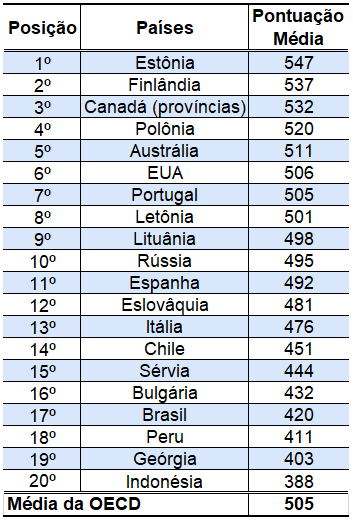
\includegraphics[width=0.6\textwidth]{tabela01-pisa2018}
\legend{\footnotesize Fonte: (\citeauthor{oecd2020}, \citeyear{oecd2020}, Table IV.1) Adaptado pelo Autor}
\label{tab:tabela01-pisa2018}
\end{minipage}
\end{table}

\newpage
As duas pesquisas descritas no parágrafo anterior demonstra que a falar sobre uso devido do dinheiro não faz parte do costume de boa parte das famílias brasileiras, principalmente, daquelas que não abordam o assunto pela falta de recursos. Segundo Fernandes e Cândido (\citeyear{fernandes-candido2014}), a falta de conhecimento financeiro causa dificuldade no controle do orçamento financeiro, fato que pode induzir ao endividamento excessivo.

Ademais, Macedo Junior (\citeyear{macedo2013}), afirma que influenciadas pelas emoções, as pessoas tomam algumas decisões de forma automática, segundo o autor, o cérebro humano possui duas estruturas mais primitivas ligadas a funções básicas de sobrevivência que afetam a tomada de decisões: o sistema límbico que controla as emoções básicas como medo, raiva e alegria e o córtex frontal que coordena o raciocínio e pensamento abstrato. Todavia, segundo Herculano-Houzel (\citeyear{herculano2005}, p. 64), “o cérebro adolescente passa por uma grande reorganização estrutural”, esse processo de reestruturação cerebral pode ser finalizado somente após os 20 anos afetando principalmente no córtex frontal, estrutura responsável pelo planejamento, controle das emoções e senso de responsabilidade \cite{konkiewitz2013}. Portanto, é muito mais complicado para um adolescente tomar decisões planejadas, por questões biológicas de desenvolvimento, inclusive as decisões financeiras, por isso, normalmente eles agem por impulso causado pelas emoções ou por repetir comportamentos e hábitos de responsáveis pela sua guarda.

Os alunos do ensino médio integrado da RFEPCT, em sua maior parte, possuem idades entre 14 a 19 anos, assim como a maior parte dos adolescentes, são mais propensos a sofrerem com endividamento excessivo, materialismo e compulsão por compras, pois tomam decisões de consumos baseados em sentimentos e emoções, pelo o fato da estrutura cerebral, responsável pelo controle da emoção e responsabilidade, ainda estar em formação. Normalmente nesta fase eles estão no início de sua vida profissional, com pouca ou nenhuma experiência sobre educação financeira, repetem os hábitos e comportamentos financeiros, comumente errôneos, dos pais ou responsáveis, amigos ou pessoas próximas, pois, aprendem por meio da imitação, em razão do seu cérebro ainda estar em desenvolvimento \cite{herculano2005} e também por não ter conhecimento aprofundado sobre finanças.

Portanto, é importante fomentar a educação financeira na formação do cidadão brasileiro como forma de provimento do letramento financeiro, para que ele possa obter conhecimento sobre o complexo sistema financeiro que interfere diretamente em sua vida. Entretanto, nos currículos dos cursos no ensino médio integrado da RFEPCT não consta a educação financeira como disciplina, exceto nos projetos pedagógicos das instituições que possuem cursos na área de finanças como os técnicos em administração, finanças e logística integrados ao ensino médio, que parcialmente adotam o ensino de finanças.

Deste modo, projetos de pesquisa que visam incentivar, desenvolver e explorar metodologias no processo de ensino e aprendizagem voltados à educação financeira são extremamente importantes para facilitar a obtenção do conhecimento, para que o estudante possa relacionar-se melhor com o dinheiro e usufruir serviços financeiros de forma consciente, contribuindo indiretamente para a estabilidade da economia nacional.

\section{ESTRUTURA DO TRABALHO}
Este trabalho está organizado em sete capítulos, com o intuito de apresentar a bases teóricas e tecnológicas necessárias para a elaboração desta dissertação.

O capítulo 1 é composto pela a introdução, a hipótese, o problema de pesquisa, os objetivos do estudo (geral e específicos), a justificativa e a descrição da estrutura do texto deste estudo.

No capítulo 2 são apresentados os trabalhos relacionados com a educação financeira, a aprendizagem através do uso de jogos como tecnologia educacional no ensino médio.

Já o capítulo 3 aborda o referencial teórico relativo aos temas fundamentais do estudo: educação financeira, as políticas da educação financeira nacional adotadas pelo governo brasileiro, a composição da RFEPCT e os institutos federais, a construção do letramento financeiro através da epistemologia genética de Jean Piaget, por derradeiro os jogos de regras e jogos sérios, principal tecnologia educacional utilizada na elaboração do presente estudo.

O capítulo 4 contempla os aspectos metodológicos de tipologia da pesquisa quanto ao campo, à sua natureza, aos objetivos, a análise dos dados, à avaliação, à finalidade e procedimentos, bem como sobre os dois jogos utilizados na pesquisa.

Em seguida, no capítulo 5 são expostos os detalhes do curso “Educação Financeira através de Jogos” produto do presente estudo, com as unidades temáticas, atividades e os conteúdos específicos para cada encontro.

O capítulo 6 relata os resultados parciais da pesquisa relacionando com os aspectos apontados no referencial teórico, por fim o capítulo 7 apresenta as considerações finais, contribuições e perspectivas futuras do presente estudo.

\chapter{ANÁLISE DOS TRABALHOS RELACIONADOS}
No intuito de averiguar a produção de trabalhos acadêmicos relacionados a cursos e a utilização de jogos no processo de ensino da educação financeira, apuradas no ensino médio do Brasil, bem como para encontrar possíveis demandas, propor e justificar a elaboração do presente trabalho e de seu produto, buscou-se encontrar estudos acadêmicos nas bases de teses e dissertações da Universidade Federal do Rio Grande do Sul (Lume), da Biblioteca Digital de Teses e Dissertações (BDTD) e do Catálogo de Teses e Dissertações da CAPES\footnote{CAPES - Coordenação de Aperfeiçoamento de Pessoal de Nível Superior}, para isso utilizou-se o termo de busca \textit{(“alfabetização financeira” \textit{OR} “letramento financeiro” \textit{OR} “educação financeira”) \textit{AND} "ensino médio".} Devido às ambiguidades nas definições dos construtos letramento financeiro, alfabetização financeira e educação financeira nos trabalhos acadêmicos (Huston, \citeyear{huston2010}; Campos, \citeyear{campos2013}), acrescentou-se ao texto da busca os termos \textit{“alfabetização financeira”} e \textit{“letramento financeiro”}, inicialmente procurou-se estudos aplicados no ensino médio integrado, contudo, por encontrar poucos estudos esta parte do termo de busca foi alterado para \textit{“ensino médio”}, tais decisões foram tomadas para aumentar o número de trabalho relacionados e qualificar o presente estudo. A busca nas bases retornou um total de 149 resultados relacionados ao termo, alguns estudos estavam presentes em mais de uma base.

O presente estudo possui como pilares a educação financeira e o ensino médio regular, por isso após a leitura do título e do resumo dos trabalhos retornados da busca, foram excluídos os seguintes estudos:

\begin{enumerate}
    \item os projetos não relacionados, diretamente, aos pilares deste estudo;
    \item os estudos voltados apenas à matemática financeira;
    \item as dissertações e teses associados à educação de adultos.
\end{enumerate}

Após as exclusões obteve-se dez dissertações de mestrado, publicadas entre o interstício de 2010 a 2019, que são consideradas trabalhos relacionados à presente pesquisa, os autores desses estudos e os respectivos títulos estão apresentados no quadro \ref{quad: quadro-01-trabalho-relacionado}.

\graphicspath{{quadros/}}
\begin{quadro}[!ht]
\centering
\begin{minipage}{1\textwidth}
\caption{Trabalhos Relacionados}
\centering
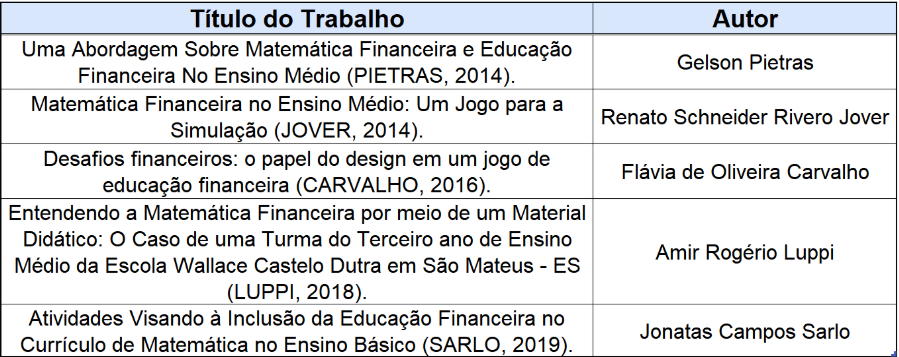
\includegraphics[width=1\textwidth]{quadro-01-trabalho-relacionado.png}
\legend{\footnotesize Fonte: O Autor, 2019}
\label{quad: quadro-01-trabalho-relacionado}
\end{minipage}
\end{quadro}

\newpage
O primeiro trabalho selecionado, ”Implicações provenientes da elaboração de um orçamento familiar” apresentado por Strate (\citeyear{strate2010}), tem o objetivo de orientar os estudantes na organização de um orçamento familiar por meio de um curso de 16 h, visando à percepção do controle financeiro na melhoria da qualidade de vida. O curso foi aplicado no Instituto de Educação Cenecista General Canabarro, localizado no município de Teutônia-RS, participaram do curso alunos com idades entre 15 e 29 anos do ensino médio e técnico da instituição. A prática pedagógica do curso apoiou-se na análise do orçamento financeiro de três colaboradores em conjunto com os alunos, posteriormente estes elaboraram o próprio orçamento, durante as aulas foi utilizado o \textit{software} ProFamília para elaboração e análise do orçamento financeiro dos colaboradores e dos alunos. O resultado do estudo destacou a importância do orçamento para melhoria da situação financeira dos discentes.

O estudo elaborado por Campos (\citeyear{campos2013}), intitulado “Investigando como a educação financeira crítica pode contribuir para a tomada de decisões de consumo de jovens-indivíduos-consumidores (JIC)”, produziu o curso de Extensão de Educação Financeira como produto educacional, baseado em situações-problemas e discussões a respeito do tema. O curso foi dividido em sete encontros e aplicado na 3ª série do ensino médio de uma escola estadual de Teófilo Otoni - MG, com tópicos relacionados ao consumo, consumismo, liberdade, manipulação, juros e o código de defesa do consumidor. No estudo o autor percebeu que, diante de algumas situações-problemas, os alunos deixavam de lado os cálculos matemáticos e decidiam as atividades financeiras baseadas em suas crenças influenciada pelo senso comum.

A dissertação de Gelson Pietras (\citeyear{pietras2014}), propõe uma abordagem para apresentação de alguns assuntos referente à educação financeira para o ensino médio, entre os quais destacam-se: matemática financeira, desejos, hábitos de consumo, poupança, dívidas, compras, capitalização e investimentos. Esses assuntos são aplicados por intermédio de uma sequência de atividades práticas para trabalhar temas como cálculos de juros, em uma dessas atividades utiliza o jogo “Banco Imobiliário” no processo de aprendizagem para que os alunos possam colocar em prática os conhecimentos adquiridos de forma lúdica. O autor concluiu que as atividades trouxeram ponderação sobre os hábitos financeiros mais comuns o que auxiliará nas próximas decisões de compra dos alunos.

Com o título “Matemática financeira no ensino médio: um Jogo para Simulação”, Renato Schneider Rivero Jover (\citeyear{jover2014}) tem o intuito de promover a educação financeira de estudantes do ensino médio com uma metodologia baseada no jogo “Investindo na Vida”, com a fundamentação teórica financeira apresentada por Robert Kiyosaki e concepções pedagógicas de Maria Montessori, Ovide, Décroly, Lev Vygotsky, Jean Piaget e Donald Winnicott, o autor também apresenta alguns artigos em sua dissertação para enfatizar a importância do lúdico na educação. A metodologia aborda o consumo, operações do mercado, ações e investimentos, assim como, aponta a importância da educação financeira para a formação social do indivíduo e a utilização jogos para auxiliar na aprendizagem.

A dissertação, “A matemática da educação financeira”, produzida por Neto (\citeyear{andreatini-neto2015}) tem o objetivo de promover nos alunos do ensino médio a reflexão acerca da educação financeira e dos conteúdos de matemática financeira por intermédio de um curso introdutório. O autor apresenta aos alunos os seguintes conteúdos: a matemática financeira, ferramentas para realizar o orçamento financeiro pessoal, obtenção e tipos de crédito pessoal e as principais aplicações financeiras em renda fixa. Neto (\citeyear{andreatini-neto2015}), propõe em seu trabalho a estrutura de um curso que deve ser aplicado ao ensino médio a partir do segundo semestre do 1º ano do ensino médio, a proposta consiste em dividir o ensino em três módulos: orçamento financeiro, serviços de créditos e aplicações em renda fixa, que deverão ser lecionados por professores de diversas áreas de conhecimento. O estudo de Neto (\citeyear{andreatini-neto2015}), considera que é obrigação da escola e da sociedade promover a educação financeira no intuito de preparar os jovens para o consumo e poupança de forma consciente.

A pesquisa apresentada por Flávia de Oliveira Carvalho (\citeyear{flavia2016}) em sua dissertação de mestrado, “Desafios financeiros: o papel do design de um jogo de educação financeira”, tem objetivo de analisar o processo de construção do jogo colaborativo “Desafio Financeiros” como material pedagógico no ensino médio, visando contribuir na formação cidadã-crítica de jovens, na faixa etária entre 14 e 18 anos, em relação aos seus hábitos de consumo. Os resultados do trabalho demonstra que o jogo contribuiu no processo de aprendizagem da educação financeira dos alunos, como material complementar à disciplina ou aplicado separadamente.

O estudo desenvolvido por Almir Rogério Luppi (\citeyear{luppi2018}), “Entendendo a matemática financeira por meio de um material didático: o caso de uma turma do terceiro ano de ensino médio da Escola Wallace Castelo Dutra em São Mateus - ES”, aborda conceitos básicos do sistema financeiro e os conteúdos oficiais da educação brasileira que focam no ensino da matemática financeira, por meio de Tecnologias da Informática e Comunicação (TICs), jogos e dinâmica em grupos. O trabalho aponta juros compostos e sistema de amortização como os tópicos mais comuns, normalmente ensinados com o auxílio da calculadora HP12C, planilhas eletrônicas ou em \textit{softwares} matemáticos como o Geogebra. Na pesquisa o autor utiliza-se do jogo “Super Banco Imobiliário” para colocar em prática, de forma lúdica, alguns conceitos sobre finanças. Luppi (\citeyear{luppi2018}) afirma que a metodologia por ele utilizada proporcionou noções importantes da matemática financeira aos alunos participantes e contribuiu para a Estratégia Nacional de Educação Financeira.

Patrícia Argôlo (\citeyear{patricia-argolo2018}) apresentou um estudo com o título “Educação financeira na sala de aula: uma proposta metodológica para o ensino da matemática no ensino médio”, a pesquisa foi aplicada em 10 encontros no Instituto Federal da Bahia no Campus Valença, com 26 alunos do 3º ano do ensino médio integrado da instituição. Durante as aulas de matemática os alunos tiveram acesso aos conteúdos relacionado à educação financeira com foco no planejamento financeiro, segundo a autora a metodologia utilizada no curso despertou o interesse dos alunos em buscar novos conhecimento sobre escolhas financeiras. Utilizando-se de atividades de planejamento financeiro, simulação de consumo, saídas a campo em mercados e mapas mentais, a autora constatou que os alunos demonstram mais interesse no assunto da aula quando os professores buscam novas práticas pedagógicas no ensino da educação financeira e da matemática financeira.

Jonatas Campos Sarlo (\citeyear{sarlo2019}) apresenta um estudo sobre a educação financeira e propõe atividades pedagógicas com recursos diferenciados como teatro, simulações de situações-problemas e jogos eletrônicos, como o “Jogo da Bolsa” com o intuito de auxiliar no desenvolvimento da autonomia do aluno em suas escolhas financeiras, bem como enriquecer as práticas pedagógicas em metodologias de ensino e aprendizagem da educação financeira. Em suas considerações finais Sarlo (\citeyear{sarlo2019}) conta que o objetivo de sua pesquisa foi alcançado com a metodologia desenvolvida, também aponta o interesse dos alunos para a temática das aulas, principalmente quando estas envolviam tecnologias digitais.

Tcharles Schneider (\citeyear{schneider2019}) apresenta o estudo “Educação Financeira: Investigação com uma Turma de 1º Ano do Ensino Médio por Meio de Práticas Colaborativas.”, o autor propôs o ensino de educação financeira nas aulas de matemática, em uma turma do 1º ano do ensino médio da Escola Estadual Nossa Senhora do Perpétuo Socorro, Município de Vera - MT, por meio de atividades de planejamento para aquisição de sonhos de consumo, com auxílio da prática colaborativa na venda de pizzas para alcançar os objetivos dos discentes. O intuito do pesquisador no estudo era discutir a influência dos grupos sociais na vida financeira, verificar processo de tomada de decisões financeiras dos alunos e explorar conceitos da matemática financeira. Schneider constatou que os jovens muitas vezes são influenciados, sem perceber, por grupos sociais nos quais convivem e concluiu que a proposta apresentou resultado satisfatório na melhoria do processo de tomada de decisão financeira dos estudantes.

Com base nos levantamentos dos estudos relacionados, no pressuposto do trabalho, no problema de pesquisa e na hipótese do presente estudo, nota-se que um curso introdutório de educação financeira deve contemplar as unidades temáticas relacionadas à matemática financeira, ao consumo consciente, aos serviços financeiros, às aplicações financeiras e às finanças comportamentais. O quadro \ref{quad: quadro-02-trabalho-relacionado_x_unidade-tematica} apresenta os trabalhos relacionado com suas respectivas unidades temáticas, tecnologia e abordagem principais.

\graphicspath{{quadros/}}
\begin{quadro}[!ht]
\centering
\begin{minipage}{1\textwidth}
\caption{Trabalhos Relacionados e Unidades Temáticas}
\centering
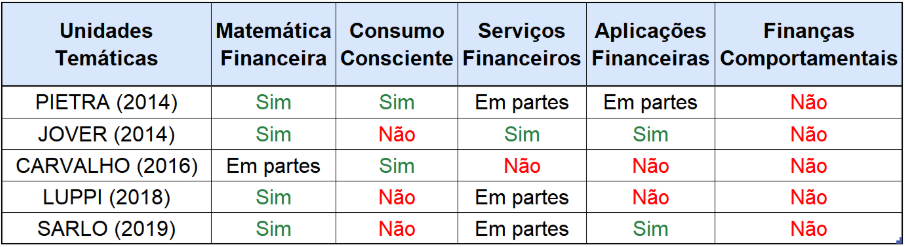
\includegraphics[width=1\textwidth]{quadro-02-trabalhos-relacionados_x_unidades-tema}
\legend{\footnotesize Fonte: O autor, 2020}
\label{quad: quadro-02-trabalho-relacionado_x_unidade-tematica}
\end{minipage}
\end{quadro}

Ao observar o quadro \ref{quad: quadro-02-trabalho-relacionado_x_unidade-tematica} e ler os trabalhos relacionados, é possível perceber uma lacuna no ensino da educação financeira a qual o presente estudo propõe solucionar, o ensino-aprendizagem de finanças comportamentais ou economia comportamental. No intuito de alcançar esse propósito, são utilizados os jogos Orçamento Consciente e Renda Passiva para reproduzir ambientes do mundo financeiro, disponibilizando por meio dos jogos situações-problemas, desafios e decisões relacionados à finança pessoal e familiar. Por intermédio da interação dos alunos com os jogos pretende-se facilitar a aprendizagem e disponibilizar um ambiente seguro para a prática dos conceitos complexos estudado, como exemplo, os aspectos psicológicos do comportamento humano. Dessa forma, auxiliar aos discentes na obtenção de conhecimento, bons hábitos e comportamentos financeiros para que possam alcançar estágios mais elevados do letramento financeiro.

\chapter{REFERENCIAL TEÓRICO}
No presente capítulo serão abordados os aspectos teóricos, epistemológicos e tecnológicos inerentes ao tema desta pesquisa, à elaboração do curso “Educação Financeira através de Jogos” do ensino médio integrado da RFEPCT e sua metodologia.

A educação financeira, as políticas públicas nacionais voltadas à educação financeira, os aspectos relevantes à epistemologia e os jogos educativos, chamados também de jogo sérios, são os principais temas do referencial teórico dos trabalhos relacionados, por isso também são explorados neste capítulo, bem como a RFEPCT, o Instituto Federal Sul-rio-grandense e seu campus na cidade de Gravataí, local onde foi aplicado à pesquisa deste estudo de caso.

\section{EDUCAÇÃO FINANCEIRA}
O Banco Central do Brasil (BACEN) é integrante do Comitê Nacional de Educação Financeira (CONEF) e uma das principais instituições do Sistema Financeiro Nacional (SFN). Segundo o BACEN (\citeyear{bacen2013}) os temas principais abordados na educação financeira são o consumo consciente (desejos x necessidades), planejamento orçamentário, crédito e dívidas, poupança e investimentos, seguros e previdência, tais assuntos estão descritos no decorrer deste item, e são objetos de estudo no processo de ensino-aprendizagem do curso “Educação Financeira através de Jogos”.

\subsection{Consumo Consciente e Finanças Comportamentais}
Segundo Buaes, Comerlato e Doll (\citeyear{buaes2015}) “entre o sonho de ter e a possibilidade de comprar é possível planejar o consumo. Esse é chamado de consumo consciente ou consumo planejado”. Em outras palavras, o consumo consciente, em finanças, compreende a utilização dos recursos de forma planejada, com planos de curto, médio e longo prazos bem definidos para evitar gastos desnecessários ou desperdício de recursos.

Entretanto, aplicar os conceitos do consumo consciente pode ser difícil, pois, as emoções e vieses interferem diretamente nas decisões financeiras das pessoas, afetando diretamente o dinheiro utilizado e o poupado \cite{martins2004}. Diante disso, é extremamente importante entender os fatores comportamentais humano relacionado ao consumo financeiro.

O estudo sobre economia comportamental é relativamente novo e engloba aspectos referentes economia e psicologia, tal conhecimento é denominada por alguns autores como finanças comportamentais. Essa área de estudo tem o objetivo de explicar a análise econômica e/ou financeira das pessoas por intermédio de pressupostos psicológicos para deliberações \cite{castro2014}, em outras palavras, as finanças comportamentais têm o interesse de explicar as tomadas de decisões financeiras das pessoas através de aspectos psicológicos do comportamento intrapessoal.

Segundo o nobelista econômico Daniel Kahneman (\citeyear{kahneman2012}) até a década de 1970 os cientistas entendiam que em geral as pessoas eram racionais e as emoções eram responsáveis por afastarem as pessoas da realidade, entretanto, o artigo escrito por Kahneman e Tversky “Julgamento sob incerteza: heurísticas e vieses” (\citeyear{kahneman1974}, tradução nossa), descreve os atalhos mentais que simplificam o pensamento de modo intuitivo e comprovam erros cognitivos do comportamento humano, não somente um simples afastamento da realidade causado pelas emoções. No artigo os autores também descreveram os vieses, erros sistemáticos e previsíveis em algumas circunstâncias, como manifestações de heurísticas, atalhos mentais que agilizam e simplificam o processo de percepção e avaliação de informações para a tomada de decisões.

Ademais, heurísticas e vieses afetam inclusive a tomada de decisões financeiras das pessoas \cite{kahneman2012}, por esse motivo, estratégias e técnicas de vendas utilizam-se destes atalhos mentais para estimular o consumidor a realizar gastos não planejados, no área do marketing estratégico tais estímulos são denominados como gatilhos mentais \cite{cialdini2012}.

Nessa perspectiva, o psicólogo Kahneman (\citeyear{kahneman2012}) sugere que o ser humano possui duas formas distintas para planejar e executar as ações: o pensamento rápido (sistema rápido) e o pensamento lento (sistema lento). O primeiro é emocional, intuitivo, impulsivo, involuntário, valoriza o presente e necessita de pouca energia do corpo humano para atuar, enquanto o segundo é racional, dedutivo, lento, consciente, valoriza o futuro e depende de mais energia das pessoas. O propósito natural do corpo de cada indivíduo é poupar energia, por isso o ser humano tende a utilizar primeiramente o pensamento rápido na tomada de decisões \cite{kahneman2012}.

Por esse motivo, as estratégias e técnicas de vendas utilizam-se dos gatilhos mentais, visando aproveitar do pensamento rápido das pessoas para estimular a aquisição de produtos e serviços. Segundo Cialdini (\citeyear{cialdini2012}), há diversos gatilhos mentais, como exemplo, o gatilho da escassez que ocorre quando um produto ou serviço é disponibilizado com poucas unidades para os clientes, ou o gatilho da urgência quando a oportunidade de compra é limitada por um pequeno interstício para o consumidor, ambos gatilhos mentais exploram um viés comportamental do ser humano, a aversão à perda (ARIELY, \citeyear{ariely2010}; KAHNEMAN, \citeyear{kahneman2012}), desta forma, os clientes são estimulados a adquirir produtos ou serviços por medo de perder uma “oportunidade”, efetuando a compra baseado instintivamente no pensamento rápido, que foi incentivado por um gatilho mental. Normalmente, o consumidor não percebe a influência destas técnicas de vendas em sua tomada de decisão no momento do consumo, as quais exploraram as heurísticas e vieses do comportamento humano, a repetição constante deste comportamento nas compras pode conduzir o consumidor ao endividamento excessivo, ao materialismo e à compulsão por compras.

Por essa razão é importante planejar o consumo a fim de obter um consumo consciente, com pouca ou nenhuma interferência das técnicas de vendas, dos gatilhos mentais, das heurísticas e vieses comportamentais, no intuito de atingir esse objetivo é extremamente importante a realização de um planejamento orçamentário.

\subsection{Planejamento Orçamentário}
O planejamento orçamentário ou orçamento financeiro é uma ferramenta para o planejamento financeiro pessoal ou familiar, o qual deve constar todas as receitas fixas e variáveis (entrada monetária), despesas fixas e variáveis (saída monetária), utilizado para decidir quais serão as prioridades de consumo pessoal ou de uma família.

\begin{citacao}
O orçamento permite o planejamento de como gastar o seu dinheiro e mesmo economizar e investir. Após listar detalhadamente todas as receitas e despesas, é preciso fazer o balanço do mês, para saber quanto sobra, quanto falta ou se há equilíbrio entre ganhos e gastos. O orçamento possibilita o planejamento financeiro, ou seja, escolher em que e como vai gastar a partir da definição de suas prioridades, além de ajudar a administrar os imprevistos e reduzir o consumo desnecessário e indesejado. \cite{buaes2015}.
\end{citacao} 

Por isso é tão importante o planejamento orçamentário na realização do consumo consciente, dos objetivos e do controle financeiro pessoal e familiar, sem o orçamento financeiro a possibilidade de ocorrer endividamento excessivo aumenta, dificultando o pagamento das dívidas, o que pode provocar a inclusão do nome em lista de proteção de crédito.

Segundo o Banco Central do Brasil (\citeyear{bacen2013}), o orçamento pode ser dividido em 4 (quatro) etapas: planejar, registrar, agrupar e avaliar as receitas e despesas pessoais ou familiar.

Planejar consiste em levantar todas as receitas e despesas, estabelecendo um limite para cada categoria de gasto, o ideal é diminuir o valor total das despesas ao máximo possível e que este não ultrapasse o valor total das receitas, pois assim sobrará mais recursos financeiros para poupar \cite{bacen2013}.

Registrar é anotar todas as despesas e receitas diárias, o que é fundamental para o planejamento orçamentário, inclusive as despesas de valores menores, visto que, somadas ao fim do mês podem gerar gastos elevados. Por muitas vezes estes valores não são considerados pelo consumidor, contudo, eles também afetam consideravelmente o orçamento. Esse registro pode ser feito através de planilhas eletrônicas, aplicativos \textit{mobile} ou qualquer \textit{software} para facilitar as anotações \cite{bacen2013}.

Agrupar significa unir as despesas e receitas anotadas em grupos, ou seja, separar cada movimentação em categorias como alimentação, moradia, saúde, mercado, compras, educação, rendimento, remuneração etc., a organização de categorias pode também ocorrer no momento do registro \cite{bacen2013}.

Por último, a avaliar se as metas máximas de consumo e receitas planejadas foram alcançadas em todas categorias, o ideal é que a soma dos gastos não ultrapasse o valor total das receitas, esta avaliação pode ser feita diariamente ou semanalmente e no final do mês \cite{bacen2013}. A repetição deste ciclo promove a continuação do consumo consciente evitando, assim, a solicitação de créditos o que pode acarretar no endividamento excessivo e na inadimplência.

\subsection{Crédito e Dívidas}
A utilização de crédito é muito comum entre a população brasileira para realizar compras de produtos, serviços, bens de consumo, imóveis, veículos etc. Contudo, o que é o crédito? Segundo o BACEN (\citeyear{bacen2013}, p. 25): “O crédito é uma fonte adicional de recursos que não são seus, mas obtidos de terceiros (bancos, financeiras, cooperativas de crédito e outros), que possibilita a antecipação do consumo para aquisição de bens ou contratação de serviços”. Em outros termos, crédito é o empréstimo de valor monetário de terceiros a consumidores quando estes não possuem ou não querem utilizar recursos próprios para aquisição de bens, serviços, produtos e outros. Existem diversas modalidades de crédito como cheque especial, empréstimos pessoais, financiamentos, cartão de crédito, crédito consignado, compra a prazo em lojas, entretanto toda a modalidade de adiantamento financeiro cobra um valor adicional além do emprestado, chamado de juros, quantia cobrada pelo aluguel do dinheiro ao consumidor que encarece o preço final \cite{bacen2013}.

A dívida é todo o compromisso financeiro realizado através de crédito em compras parceladas de produtos, serviços, bens de consumo, imóveis etc., o excesso de dívidas, a falta de consumo consciente e de um plano orçamentário pode acarretar no atraso de pagamentos, ou pior, o não pagamento das dívidas e neste momento o consumidor tornar-se-á inadimplente, passível de ter o seu nome inscrito em órgãos de proteção ao crédito como o SCPC (Serviço Central de Proteção ao Crédito), o que dificultará a obtenção de novos créditos. Para Gustavo Cerbasi (\citeyear{cerbasi2015}), a melhor forma de comprar um produto ou serviço é poupar e investir mensalmente até obter o valor total do item, evitando contratar créditos que comprometem o poder de compra dos meses posteriores.

A tomada de crédito pelos consumidores tem crescido anualmente no Brasil, causando um aumento no número de endividados \cite{cnc2020}, segundo Bortoluzzi et al (\citeyear{bortoluzzi2015}), a partir de 2003 o Brasil sofreu transformações no modelo econômico e social, as quais possibilitaram grandes mudanças para a sociedade brasileira. Nesse modelo as medidas políticas propuseram redução na taxa de juros, ampliação do volume de crédito direcionado às empresas e às famílias, tornando o crédito mais acessível à população. Entretanto, os autores apontam que esta facilidade de acesso ao crédito em conjunto com a falta da educação financeira provocaram um aumento no índice de endividamento. Nessa perspectiva, a facilidade na contratação de crédito, a falta da educação financeira e o grande apelo ao consumo do marketing, pode transformar-se em armadilha para o consumidor, pois de acordo com Zaremba (\citeyear{zaremba2007}), a maior parte das pessoas age como se não conhecesse que pagar juros abusivos podem acarretar em problemas financeiros.

\subsection{Poupança e Investimentos}
O resultado do orçamento pessoal ou familiar pode ser avaliado, de forma geral, calculando a diferença entre o total de entrada monetária (receita) e o total de saída monetária (despesa). Desta forma quando:

\begin{itemize}
    \item A despesa for maior que a receita o orçamento será deficitário;
    \item A despesa for igual a receita o orçamento será neutro;
    \item A receita for maior que a despesa o orçamento será superavitário.
\end{itemize}

Segundo o Banco do Brasil (\citeyear{bb2012}, p. 24): “Quando a pessoa não consome toda a sua renda, essa sobra poderá ser transformada em poupança”, portanto todo orçamento superavitário produz uma sobra financeira chamada de poupança, normalmente confundido com Caderneta de Poupança que é a aplicação mais popular no Brasil.

O investimento ou aplicação ocorre quando o dinheiro poupado é utilizado para gerar mais dinheiro, por isso é considerado um ativo. Existem diversos tipos de aplicações financeiras no Brasil, as mais comuns são a Caderneta de Poupança, Certificados de Depósito Bancário (CDB), Recibo de Depósito Bancário (RDB), Letras de Crédito (LC), Letras de Crédito Imobiliário (LCI) e Letras de Crédito do Agronegócio (LCA), Debêntures, Títulos Públicos, Ações, Fundos e Clubes de Investimentos.

Todo o investimento possui três componentes: liquidez, risco e rentabilidade. De acordo com BACEN (\citeyear{bacen2013}), a liquidez é a capacidade de um investimento ser transformado em dinheiro, em qualquer tempo por um preço justo. O risco é a possibilidade de ocorrer perda no valor investido e a rentabilidade é a remuneração que o investimento retorna ao investidor. Quanto maior o risco, maior é a possibilidade de ocorrer perdas de capital, entretanto maior poderá ser a rentabilidade da aplicação.

Quanto a rentabilidade, os investimentos se caracterizam como renda fixa ou renda variável. Na renda fixa a remuneração paga é correspondente a uma taxa de juros determinada na contratação, já na renda variável não é possível determinar uma taxa de remuneração na contração \cite{bacen2013}. Em outras palavras, o investidor que contrata uma aplicação de renda fixa sabe qual será a taxa de juros acordada, ao contrário da renda variável onde a rentabilidade será determinada no momento da venda do ativo, o que pode, inclusive, incorrer em perdas no montante aplicado. Ao realizar um plano de investimento é importante considerar o risco, a liquidez, a rentabilidade, o tipo da aplicação e a finalidade de uso dos recursos alocados de acordo com o objetivo de cada investidor.

\subsection{Seguros e Previdência}
A Superintendência de Seguros Privados (Susep), órgão federal brasileiro responsável por fiscalizar e controlar empresas de seguros e previdência privada, afirma que seguro é o:

\begin{citacao}
Contrato mediante o qual uma pessoa denominada Segurador, se obriga, mediante o recebimento de um prêmio, a indenizar outra pessoa, denominada Segurado, do prejuízo resultante de riscos futuros, previstos no contrato \cite{susep2007}.
\end{citacao}

A vida é imprevisível, em boa parte, eventos (positivos ou negativo) não planejados, inesperados ou impensáveis podem ocorrer com qualquer ser humano, entre os eventos ruins pode-se citar exemplos como: doenças, acidentes, morte, desemprego, furtos ou roubos de bens entre outros. Por isso, a importância da contratação de um seguro, com objetivo de diminuir o prejuízo financeiro causado por eventuais problemas inesperados. Para isso, as seguradoras oferecem diversos tipos de seguros com respectivos planos, benefícios e contratos, entre os principais destacam-se o de vida, residencial, veicular, empresarial e viagem.

Da mesma forma, a previdência em finanças é a preparação econômica durante um determinado período para lidar com situações do futuro como aposentadoria ou realização de projetos \cite{bb2015}. Atualmente existem dois tipos de regimes para prover recursos financeiros: a Previdência Social, administrada pelo Instituto Nacional de Seguro Social, e a Previdência Privada, oferecida por bancos e seguradoras e supervisionadas pela Susep.

\section{POLÍTICAS DA EDUCAÇÃO FINANCEIRA NACIONAL}
O intuito deste capítulo é apresentar o levantamento das políticas públicas educacionais no Brasil voltadas ao desenvolvimento da educação financeira na educação básica regular, especificamente os projetos de leis sobre a educação financeira que tramitam no Congresso Nacional, a Estratégia Nacional de Educação Financeira - ENEF e as propostas da Base Nacional Comum Curricular - BNCC para o ensino de finanças na educação básica.

\subsection{Projetos de Lei Sobre a Educação Financeira}
Analisando o site da Câmara dos Deputados, casa iniciadora de leis no Brasil, nota-se a existência de 12 projetos de lei, discutidos entre os anos de 2004 a 2020, cujo conteúdo propõe a inclusão da educação financeira como componente curricular na educação básica (ensino fundamental e médio). Neste levantamento considerou-se apenas os projetos da Câmara dos Deputados, por ser a casa iniciadora das leis federais.

O primeiro Projeto de Lei o PL 3401/2004 foi arquivado, tal como o PL 306/2007, outros nove projetos discutidos (PL 3421/2012, PL 7155/2014, PL 3590/2015, PL 3691/2015, PL 4215/2015, PL 4915/2016, PL 7318/2017, PL 239/2019, PL 3114/2019), por tratarem de temáticas idênticas, foram apensados (unidos), diretamente ou indiretamente, ao PL 2107/2011, que encontra-se na Comissão de Educação (CE), sendo este projeto o único em pauta no Congresso Nacional, tornando-o principal relacionado à inclusão da educação financeira na educação básica.

O Projeto de Lei PL 2107/2011 possui como proposta “alterar a lei de diretrizes e bases da educação nacional, incluindo a disciplina de Noções de Educação Financeira como conteúdo obrigatório no ensino médio” \cite{brasil2011}. Além disso, estabelece o interstício de 3 anos para os sistemas de ensino se adequarem às exigências descritas \cite{brasil2011}, todavia, não aborda a educação financeira para o ensino fundamental.

Ao analisar o histórico dos projetos de lei voltados à educação financeira observa-se que o primeiro trabalho foi proposto em 2004, há 16 anos, até a elaboração deste estudo nenhum projeto foi transformado em lei. A falta de celeridade na aprovação de uma lei, que torna a educação financeira obrigatória no ensino básico, não condiz com a relevância do tema, o qual contribui para a estabilidade econômica, o bem-estar social dos brasileiros e a formação cidadã dos estudantes.

\subsection{A Estratégia Nacional de Educação Financeira}
Entre as diversas iniciativas para promover o letramento financeiro no Brasil destaca-se a criação da Estratégia Nacional de Educação Financeira (ENEF), instituída pelo governo brasileiro através do Decreto nº7.397, de 22 de dezembro de 2010, sob a responsabilidade do Comitê Nacional de Educação Financeira (CONEF), com a execução e coordenação dos programas realizadas pela Associação de Educação Financeira do Brasil (AEF-Brasil). Tal estratégia tem a finalidade de fortalecer a cidadania, aumentar a eficiência e solidez do Sistema Financeiro Nacional (SFN), disseminar a educação financeira e previdenciária, promover as decisões financeiras de forma consciente e autônoma, bem como atuar com informação, orientação e formação de forma gratuita visando o interesse público, por intermédio de dois documentos norteadores: Orientações para Educação Financeira nas Escolas e Orientações para Educação Financeira de Adultos \cite{enef2010}. Através da ENEF são executados projetos de cursos, blogs, vídeos, livros, jogos, material de apoio aos professores do ensino médio e fundamental, a Semana da Educação Financeira e o Mapeamento de Iniciativas de Educação Financeira voltadas para o desenvolvimento da educação financeira no Brasil.

O CONEF, também constituído pelo Decreto nº7.397, é composto pelo Diretor do Banco do Brasil, Presidente da Comissão de Valores Mobiliários, Diretor-Superintendente da Superintendência Nacional de Previdência Complementar, Superintendente da Superintendência de Seguros Privados, Secretário-Executivo do Ministério da Fazenda, Secretário-Executivo do Ministério da Educação, Secretário-Executivo do Ministério do Trabalho e Previdência Social e o Secretário Nacional do Consumidor do Ministério da Justiça. Observa-se na composição do CONEF a presença dos principais órgãos federais relacionados às finanças, economia e trabalho. Compete ao CONEF promover a educação financeira através de planos, metas, programas, ações, financiamento, execução de projetos e revisão da ENEF \cite{brasil2010}.

A AEF-Brasil é uma Organização da Sociedade Civil de Interesse Público (OSCIP), com certificação do Ministério da Justiça, composta por quatro instituições do mercado financeiro: Associação Brasileira das Entidades dos Mercados Financeiros e de Capitais (ANBIMA); Brasil, Bolsa, Balcão (B3); Confederação Nacional das Empresas de Seguros Gerais, Previdência Privada e Vida, Saúde Suplementar e Capitalização (CNSeg); e Federação Brasileira de Bancos (FEBRABAN). Por convênio de cooperação técnica com o CONEF, a AEF-Brasil é responsável por executar e coordenar todos os programas propostos pela ENEF e tem o objetivo de promover a educação financeira nacional e de tecnologias socioeducacionais nesta área \cite{aefbrasil2011}. A AEF-Brasil é uma associação sem fim lucrativo e recebe apoio financeiro de instituições privadas, do governo e da sociedade civil que compreendem a importância da educação financeira.

Recentemente o governo brasileiro, por meio do Decreto Nº 10.393, de 9 de junho de 2020, instituiu a nova Estratégia Nacional da Educação Financeira e o Fórum Brasileiro de Educação Financeira - FBEF, revogando o Decreto nº7.397/2010, com a promulgação do novo decreto, o FBEF tornou-se responsável por promover, executar e coordenar as ações de educação financeira e previdenciária da ENEF e também da educação securitária e fiscal, estes últimos incluídos pelo novo decreto \cite{brasil2020}.

O FBEF é composta por representantes dos Banco Central do Brasil, Comissão de Valores Mobiliários, Superintendência de Seguros Privados, Secretaria do Tesouro Nacional da Secretaria Especial de Fazenda do Ministério da Economia, Secretaria de Previdência da Secretaria Especial de Previdência e Trabalho do Ministério da Economia, Superintendência Nacional de Previdência Complementar, Secretaria Nacional do Consumidor do Ministério da Justiça e Segurança Pública e Ministério da Educação, ao FBEF compete:

\begin{citacao}
    \begin{itemize}
        \item implementar e estabelecer os princípios da ENEF;
        \item divulgar as ações de educação financeira, securitária, previdenciária e fiscal propostas por seus membros, por outros órgãos e entidades públicas ou por instituições privadas;
        \item compartilhar as informações sobre as ações de educação financeira, securitária, previdenciária e fiscal produzidas pelos órgãos e entidades representados, para identificar as oportunidades de articulação; e
        \item promover a interlocução entre os órgãos ou as entidades públicas e as instituições privadas para estimular e, sempre que possível, integrar as ações de educação financeira, securitária, previdenciária e fiscal. \cite{brasil2020}.
    \end{itemize}
\end{citacao}

De acordo com o novo decreto, “a presidência do FBEF será exercida, a cada período de vinte e quatro meses, por um de seus membros.” \cite{brasil2020} e as reuniões ocorrerão ordinariamente uma vez por semestre e extraordinariamente sempre que convocado pelo seu Presidente ou pela maioria de seus membros. O FBEF poderá instituir até quatro grupos de trabalhos simultâneos, com duração máxima de um ano para cada grupo a fim de examinar assuntos específicos e fornecer suporte técnico sobre a promoção da educação financeira, securitária, previdenciária e fiscal brasileira.

\subsection{A BNCC e a Educação Financeira}
A Constituição do Brasil de 1988 prevê a elaboração de conteúdos mínimos para o ensino básico a fim de assegurar formação comum nacional, entretanto somente em 1996 foi aprovada a Lei 9.394/1996 que regula a base nacional comum para o ensino básico em todos sistemas de ensino \cite{brasil1996}. Entre os anos 1997 a 2012 são lançados os Parâmetros Curriculares Nacionais (PCN), as Diretrizes Curriculares Nacionais Gerais para o ensino básico (DCNs) e os Parâmetros Curriculares Nacionais para o Ensino Médio (PCNEM) “com o objetivo de cumprir o duplo papel de difundir os princípios da reforma curricular e orientar o professor, na busca de novas abordagens e metodologias.” \cite{brasil2017b}, entretanto, nenhum desses documentos faz menção a educação financeira. Em 2014 o Ministério da Educação e Cultura iniciou a elaboração da BNCC visando estabelecer os ensinamentos básicos para o desenvolvimento de conhecimentos necessários para o exercício da cidadania. No ano de 2015 foi disponibilizada a primeira versão da BNCC, consequentemente, iniciou-se uma mobilização entre as instituições de ensino para a discussão sobre a BNCC. Após dois anos de debates e mudanças, a BNCC foi homologada pelo Ministério da Educação (MEC) em 2017 para o ensino fundamental e em 2018 para o ensino médio, a base comum nacional  apresenta orientações sobre conceitos básicos da educação financeira como economia, finanças, taxas de juros, inflação, aplicações financeiras e impostos, com o intuito de unificar o processo de ensino-aprendizagem, além de tornar o ensino da educação financeira obrigatório em todas as instituições de ensino a partir de 2020.

Segundo a BNCC \cite{brasil2017a}, nas séries iniciais do ensino fundamental, do 1ª ao 4ª ano, deve-se trabalhar com os estudantes especificamente a unidade temática “Grandezas e Medidas” concentrando-se no reconhecimento, conversões e resolução de problemas do sistema monetário brasileiro, habilidades estas que estão ligadas à matemática financeira. A partir do 6º ano, o tema retorna ao currículo e permanece até o fim do ensino fundamental através das unidades temáticas “Números” e “Grandezas e Medidas”, trabalhando as habilidades da BNCC descritas nos códigos EF06MA13, EF06MA32, EF07MA02, EF07MA02 e a EF09MA05 que descreve:

\begin{citacao}
Resolver e elaborar problemas que envolvam porcentagens, com a ideia de aplicação de percentuais sucessivos e a determinação das taxas percentuais, preferencialmente com o uso de tecnologias digitais, no contexto da educação financeira. \cite{brasil2017a}.
\end{citacao}

A habilidade EF09MA05 é indicada na BNCC ao 9º ano do ensino fundamental e aborda parte da educação financeira através de uma metodologia ativa de resolução de problemas com apoio da tecnologia, o que poderá trazer estímulos maiores para aprendizagem, principalmente se o contexto do problema proposto fizer parte do cotidiano do aluno.

No mesmo sentido, no ensino médio a BNCC apresenta a matemática financeira e parcialmente a educação financeira por meio de temas ligados a finanças pessoais e familiares como orçamento, investimentos, sustentabilidade e tomada de decisões, também com apoio de tecnologias digitais através das habilidades descritas no quadro \ref{quad: quadro-03-habilidade}.

\graphicspath{{quadros/}}
\begin{quadro}[!ht]
\centering
\begin{minipage}{1.\textwidth}
\caption{Habilidades Propostas para Matemática e Educação Financeira}
\centering
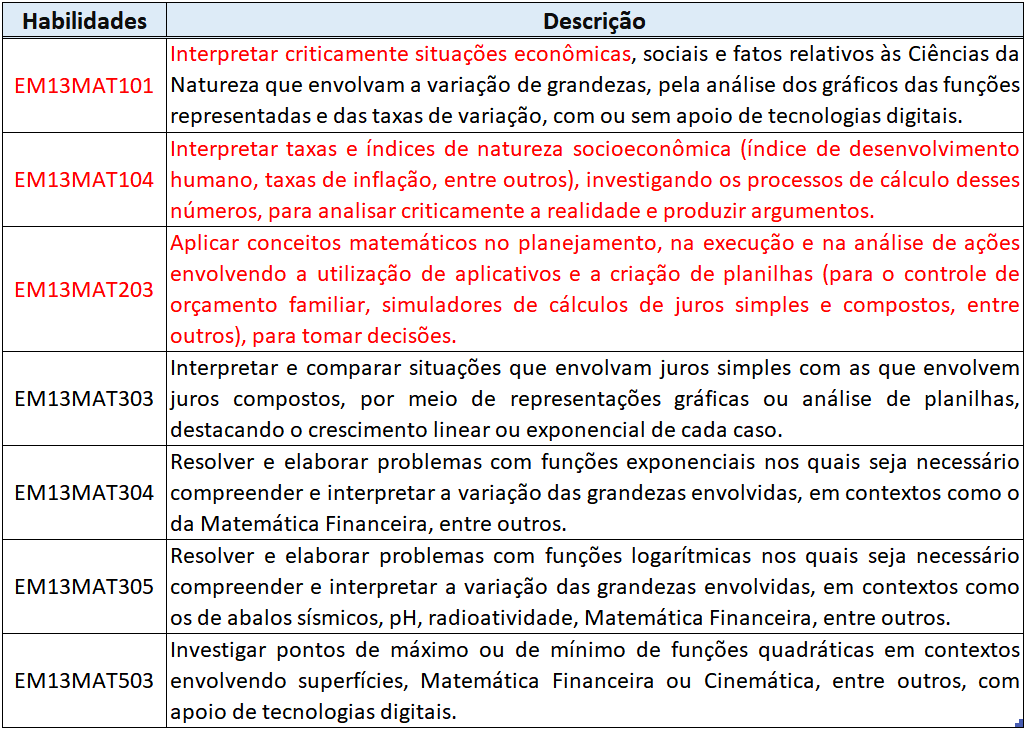
\includegraphics[width=1\textwidth]{quadro-03-habilidades}
\legend{\footnotesize Fonte: \cite{bncc2018} Adaptado pelo Autor}
\label{quad: quadro-03-habilidade}
\end{minipage}
\end{quadro}

Analisando o quadro \ref{quad: quadro-03-habilidade} nota-se que as habilidades descritas e propostas na BNCC, em sua maior parte, são voltadas ao contexto da matemática financeira, exceto as habilidades EM13MAT101, EM13MAT104 e EM13MAT203, destacadas em vermelho no quadro, que abordam parcialmente a educação financeira.

A Base Nacional Comum Curricular apresentou pequenos avanços no incentivo a construção da educação financeira, principalmente na unidade temática relacionada à matemática financeira, por meio da inclusão de habilidades relacionadas a cálculos e funções matemáticas, todavia, Kahneman (\citeyear{kahneman2012}) afirma que pessoas podem ter a capacidade realizar cálculos financeiros com exatidão e concomitantemente ter comportamento e hábitos que lhes trazem problemas com finanças. Desse modo, o indivíduo pode ser um exímio matemático financeiro e, ainda assim, possuir fatores comportamentais que induzem ao materialismo, à compulsividade em compras e à propensão ao endividamento. Por isso, é importante aos alunos da educação básica a aprendizagem integral da educação financeira a qual engloba todas as suas unidades temáticas (matemática financeira, finanças comportamentais, consumo consciente, instituições financeiras, investimento e previdência). Desta forma, pode-se proporcionar aos alunos conhecimentos para exercer melhores escolhas financeiras para melhoria em sua qualidade de vida e bem-estar social fortalecendo assim a cidadania do país.

\section{A RFEPCT E OS INSTITUTOS FEDERAIS}
Os Institutos Federais de Educação, Ciência e Tecnologia foram instituídos com a promulgação da Lei 11.892 em 2008, os institutos fazem parte da Rede Federal de Educação Profissional, Científica e Tecnológica que foi formalmente oficializada por meio da mesma lei. A RFEPCT é formada por um conjunto de autarquias da administração pública indireta que possuem autonomia administrativa, patrimonial, financeira, didático-pedagógica e disciplinar, sendo composta pelas seguintes instituições \cite{brasil2008}:

\begin{itemize}
    \item 38 Institutos Federais de Educação, Ciência e Tecnologia
    \item 3 Centros Federais de Educação Tecnológica
    \item 23 Escolas, Colégios, Centros vinculados às Universidades Federais
    \item Universidade Tecnológica Federal do Paraná
    \item Colégio Pedro II
\end{itemize}

Cada instituto federal tem por objetivos: ministrar educação profissional técnica de nível médio nos formatos integrado, subsequente e concomitante, privilegiando os cursos integrados, reservando no mínimo 50\% para este objetivo; realizar projetos de extensão e pesquisas aplicadas; ministrar em nível de educação superior cursos de bacharelado, tecnologia e licenciatura, bem como pós-graduação \textit{lato sensu} e \textit{stricto sensu} de mestrado e doutorado. Os objetivos dos cursos devem estar em articulação com o mundo do trabalho, a sociedade e o desenvolvimento socioeconômico local e regional, nas áreas da educação profissional e tecnológica \cite{brasil2008}.

A tabela \ref{tab: tabela02-institutos} apresenta a disposição dos Institutos Federais de Educação, Ciência e Tecnologia, Colégio Pedro II, Centros Federais de Educação Tecnológica e seus campi. São ao todo 42 instituições com 632 campus que podem ministrar a educação profissional técnica de nível médio no formato integrado.

\newpage
\graphicspath{{tabelas/}}
\begin{table}[!ht]
\centering
\begin{minipage}{1.\textwidth}
\caption{Disposição das Instituições de Ensino da RFEPCT}
\centering
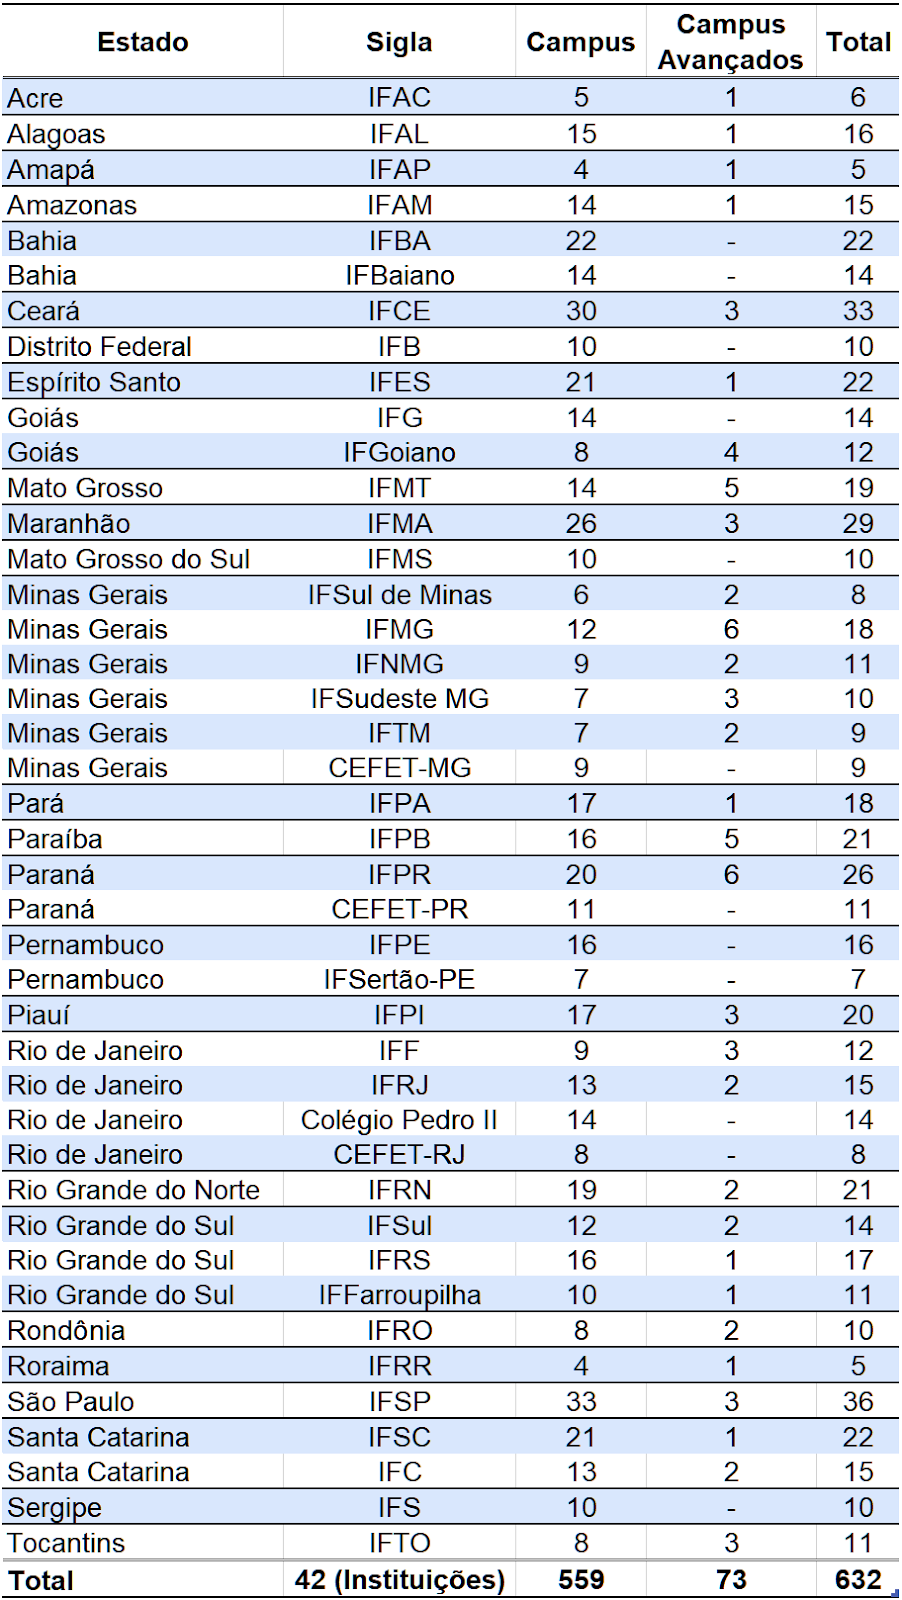
\includegraphics[width=0.7\textwidth]{tabela02-institutos.png}
\legend{\footnotesize Fonte: Dados pesquisados nos portais das instituições}
\label{tab: tabela02-institutos}
\end{minipage}
\end{table}

Dentro das diversas instituições de ensino da RFEPCT, listados na tabela \ref{tab: tabela02-institutos}, há o Instituto Federal Sul-rio-grandense-IFSUL local onde foi aplicada à pesquisa do presente estudo, especificamente no Campus Gravataí.

\section{APRENDIZAGEM, JOGOS E A EDUCAÇÃO FINANCEIRA}
A educação financeira tem por objetivo o desenvolvimento de novos conhecimentos sobre bons hábitos e comportamentos a fim de obter um bom letramento financeiro, podendo ocorrer essa educação por intermédio de um processo de ensino-aprendizagem.

No propósito de propor um processo educacional para a educação financeira, este trabalho se fundamenta nas teorias de aprendizagem do epistemólogo Jean Piaget para estruturar meios e recursos no intuito de encontrar um bom caminho para o processo de ensino-aprendizagem da educação financeira e promover letramento financeiro aos alunos da RFEPCT.

Ao buscar informações sobre educação financeira, são encontradas inúmeras fontes de livros, sites, vídeos, \textit{blogs}, cursos, entre outros, sobre planejamento financeiro orçamentário, sonhos, objetivos, metas, planos, aposentadoria, despesas, receitas, dívidas, gastos, poupança, aplicações financeiras, hábitos e finanças comportamentais. Consumir todas essas informações disponíveis pode exigir do sujeito um saber antecipado para o desenvolvimento de sua aprendizagem, o que é capaz de dificultar a formação de estruturas cognitivas básicas necessárias para transformação da informação em conhecimento prático \cite{piaget2011}. 

Tendo em vista a importância de se estabelecer um caminho para a aprendizagem, esta seção apresenta uma via de acesso para a construção do conhecimento sobre a educação financeira, procurando correlacionar os estágios da aprendizagem do letramento financeiro com os estágios do desenvolvimento cognitivo propostos por Piaget, assim como, discorre sobre a importância e utilização de jogos no processo de ensino-aprendizagem através de alguns estudos, no intuito de incentivar desenvolvimento do letramento financeiro nos estudantes.

\subsection{Os Estágios do Letramento Financeiro com Base em Piaget}
Piaget (\citeyear{piaget1971}) propõe que o desenvolvimento cognitivo de uma criança possui 4 níveis ou estágios (sensório motor, pré-operatório, operatório concreto e operatório formal) com características específicas em cada uma das fases, como a idade dos indivíduos. Segundo a teoria piagetiana, o sujeito atinge o estágio operacional formal a partir dos 12 anos, entretanto, quando se trata de um tema desconhecido e distante do sujeito, observam-se ações, atitudes e interações semelhantes aos primeiros estágios do desenvolvimento cognitivo, mesmo em sujeitos que por sua idade e maturação atingiram o último estágio (operacional formal), desta forma, quando o sujeito necessita adquirir um novo conhecimento, distante de si, ele transita dos estágios iniciais até o final por meio de diversos processos de assimilação, acomodação, adaptação e equilíbrio para adquirir o novo saber, bem como colocá-lo em prática, fato que também ocorre no processo de desenvolvimento do letramento financeiro do sujeito, independentemente da sua idade e maturação.

O primeiro estágio proposto por Piaget (\citeyear{piaget1971}) é o sensório motor. Nessa fase a criança começa a construir esquemas para assimilar o meio através de percepções sensoriais e esquemas motores, é a inteligência prática do “aqui e agora”. Nesta etapa a criança não apresenta nenhuma conduta em relação aos objetos que desaparecem do seu campo visual, por isso não compreende nem sabe para onde o objeto foi, normalmente continuam procurando-o no local onde o objeto desapareceu e não compreende que este continua existindo em outro local, ocorre também reações circulares secundárias onde qualquer ação que leva ao um fim agradável é repetida intencionalmente. De modo análogo, no desenvolvimento cognitivo do letramento financeiro dentro do primeiro estágio o sujeito repetidamente troca seu dinheiro baseado em sentimentos agradáveis que a compra lhe proporciona. Segundo Figueira (\citeyear{figueira2014}), estas sensações geram “prazer nas compras”, um dos fatores que contribuem para o consumidor realizar compras compulsivamente, o que pode gerar um endividamento excessivo. Em diversas ocasiões as sensações são iniciadas por estratégias de vendas baseadas em gatilhos (atalhos) mentais, o sujeito repete intencionalmente a ação e não percebe que o dinheiro diminui a cada gasto, sem saber também o destino do dinheiro quando questionado, pois não há qualquer controle ou administração, o salário termina e ele não tem ideia com que gastou. Define-se esse estágio no letramento financeiros como o Consumidor Sensorial (PERES et al., \citeyear{peres2019}), nele o sujeito normalmente lida com o dinheiro através da inteligência prática do “aqui e agora” utiliza todo o dinheiro que ganha mensalmente, muitas vezes recorrendo a empréstimos, se necessário, no intuito de suprir seus desejos, para o sujeito nesse estágio, dinheiro é apenas um objeto de troca para obter sensações agradáveis. Normalmente neste estágio o sujeito não poupa para uma emergência ou oportunidade, gastando sem estabelecer um plano orçamentário, não registra os gastos e receitas mensais, por isso tem dificuldade em observar e saber o destino do dinheiro utilizado.

O segundo estágio proposto por Piaget (\citeyear{piaget1971}) é o pré-operatório, nessa fase a criança desenvolve o domínio da linguagem e da representação, possui característica da função simbólica (consegue gerar imagem mental e representar), jogo simbólico (brincadeira de faz de conta), desenhos e o pensamento intuitivo (conhecimento baseado na percepção, ainda não compreende a irreversibilidade), entre outros. Da mesma forma no segundo estágio de desenvolvimento cognitivo do letramento financeiro o sujeito começa a desenvolver o domínio sobre o dinheiro e sensações que impulsionam seus gastos, ele consegue compreender que o dinheiro é um símbolo e na verdade representa o tempo de vida que se usa para obtê-lo, portanto, entende que um produto ou serviço é pago com tempo de vida e não com dinheiro. Geralmente por causa do desequilíbrio financeiro do estágio anterior começa a realizar anotações de despesas, receitas, desenhar um orçamento e estudar sobre educação financeira para poder assimilar, acomodar e adaptar os novos conhecimentos e assim realizar o equilíbrio do conhecimento financeiro, aprende também, a viver de acordo com seu nível financeiro, em outras palavras, gastar somente aquilo que ganha. Neste estágio o sujeito já pensa e representa seus sonhos e objetivos em relação ao dinheiro, todavia não consegue elaborar metas e realizá-las, pois não compreende ainda a irreversibilidade de suas atitudes financeiras, por isso, ainda não aplica seus recursos financeiros para conseguir alcançar seus sonhos e objetivos. Define-se esse estágio como o Consumidor Pré-Poupador (PERES et al., \citeyear{peres2019}), normalmente nesse estágio o sujeito não poupa dinheiro para objetivos de curto, médio e longo prazo como a aposentadoria, honra os compromissos financeiros com facilidade, não separa parte do dinheiro ganho para investir, por fim utiliza de todos os recursos financeiros adquiridos mensalmente.

O terceiro estágio proposto por Piaget (\citeyear{piaget1971}) é o operatório concreto nessa fase o pensamento do sujeito é lógico, objetivo e reversível, nesse estágio a criança não se limita a uma representação imediata, mas ainda depende do mundo concreto para chegar à abstração. De igual modo no terceiro estágio do letramento financeiro o sujeito desenvolve o pensamento lógico, objetivo e reversível. Através desse pensamento, compreende a necessidade de poupar dinheiro para os objetivos, desejos, imprevistos, oportunidades e entende a importância de adquirir serviços de seguros, entretanto, ainda não consegue elaborar projetos, metas e prazos para alcançar seus sonhos e objetivos. Define-se este estágio como o Poupador Concreto (PERES et al., \citeyear{peres2019}), nesse estágio o sujeito realiza o controle efetivo das receitas e despesas pessoais e familiar, vive no mínimo um nível financeiro abaixo da sua renda, em outras palavras, suas despesas mensais são sempre menores que as receitas, obtendo assim um orçamento superavitário, poupando dinheiro na maior parte dos meses. Normalmente nesse estágio o sujeito aplica o dinheiro que sobrou em uma caderneta de poupança, por falta de conhecimento em outros investimentos e pelo contexto histórico financeiro brasileiro, onde a população tem preferência por este tipo de aplicação, também não define metas de curto, médio e longo prazo para o dinheiro poupado, apenas guarda o dinheiro que poupou.

O quarto estágio proposto por Piaget (\citeyear{piaget1971}) é o operatório formal, nessa fase a criança desenvolve o pensamento hipotético-dedutivo, bem como a consolidação da personalidade, socialização, autonomia, moralidade, liberdade e direitos. Igualmente, no quarto estágio do desenvolvimento cognitivo do letramento financeiro, o sujeito desenvolve o pensamento hipotético-dedutivo, desta forma consegue abstrair seus sonhos e objetivos financeiros criando metas de curto, médio e longo prazo para alcançá-los com o dinheiro poupado mensalmente, também consolida a personalidade de investidor (conservador, moderado ou arrojado), a socialização para aprender e ensinar mais sobre finanças, a autonomia e a liberdade para decidir suas escolhas financeiras para o dinheiro poupado por causa do conhecimento adquirido. Define-se esse estágio como o Investidor Formal (PERES et al., \citeyear{peres2019}), nesse estágio o sujeito estabelece planos com prazos e metas bem definidos para alcançar seus objetivos financeiros, reconhece seu perfil de investidor e consome os melhores serviços financeiros de acordo com seu conhecimento e objetivos desejados, busca constantemente obter novos conhecimentos sobre letramento financeiro, entende e utiliza seus direitos, bem como cumpre com suas obrigações financeiras. Normalmente o sujeito estágio Investidor Formal possui o montante investido para reserva de emergência ou oportunidade, poupa parte do dinheiro recebido mensalmente para realizar seus sonhos e objetivos, registra objetivos e metas de curto, médio e longo prazo, não possui dívidas ou as têm sob controle, reconhece seu perfil de investidor e aplica o dinheiro poupado em diversos investimentos de acordo com seu perfil, metas, objetivos e aplicações disponíveis.

Para ascender os estágios do letramento financeiro é necessário que o sujeito coloque em prática os conceitos aprendidos, por intermédio da reflexão, alteração e aplicação de bons hábitos e comportamentos financeiros. Os jogos podem ser utilizados para promover um ambiente seguro para a prática dos novos conhecimentos, hábitos e comportamentos financeiros adquiridos, o que favorece a aprendizagem, por isso, a próxima seção abordará a influência dos jogos na aprendizagem.

\subsection{A Utilização de Jogos na Aprendizagem}
Os jogos estão presentes na rotina atual de adolescentes, jovens e adultos brasileiros, inicialmente para entretenimento, segundo o grupo NPD (\citeyear{npd2015}), empresa americana de pesquisa de mercado, cerca de 82\% da população brasileira com idades entre 13 e 59 anos utiliza diversas plataformas digitais para jogar, seja em computadores, consoles de videogames, dispositivos móveis ou portáteis, esta pesquisa demonstra o impacto dos jogos no Brasil.

Segundo o historiador Johan Huizinga (\citeyear{huizinga2000}) o jogo precede a cultura e por ela tem seu significado alterado, portanto, a relação do homem com o jogo é antiga e antecede a cultura humana. O pesquisador acrescenta que existe uma espécie de “instinto de jogo” no ser humano de todas as idades, o que torna o jogo uma atividade natural do homem para se divertir e se preparar para trabalhos futuros.

Por esse motivo, os jogos são estudados por diversos pesquisadores e possuem diferentes classificações.  Para Jean Piaget (\citeyear{piaget1969}) os jogos podem ser um excelente recurso para desenvolvimento sócio-cognitivo do indivíduo e no processo de aprendizagem, por isso em seus estudos o pesquisador elaborou uma classificação dos jogos separando-os em três categorias relacionadas aos estágios do desenvolvimento infantil, na seguinte forma:

\begin{itemize}
    \item Jogos de exercícios - a partir do estágio sensório motor;
    \item Jogos simbólicos - a partir do estágio pré-operatório;
    \item Jogos de regras - a partir do estágio operatório concreto.
\end{itemize}

De acordo com Piaget (\citeyear{piaget1969}), o jogo de exercício compreende a realização repetida de movimentos e gestos simples como agitar membros, balançar objetos, emitir sons, andar, correr, pular, entre outros; no jogo simbólico o sujeito transforma o ambiente real por meio do faz-de-conta para satisfazer seus desejos, esse tipo de jogo possibilita o sujeito externar a realização de sonhos e fantasias, bem como revela conflitos, medos e angústias; o jogo de regras caracteriza-se pelo conjunto de normas e obrigações impostas pelos jogadores, o descumprimento dessas regras normalmente gera uma penalidade ao jogador, os jogos de regras normalmente proporciona uma forte competição entre os indivíduos. Segundo Piaget (\citeyear{piaget1969}), o jogo de regras inicia-se na vida do sujeito por volta dos 5 anos, se fortalece entre os 7 e 12 anos e continua durante toda a vida na fase adulta no esporte, trabalho, entre outros. Ademais, o autor classifica os jogos de regras em dois tipos: jogos de exercício sensório-motor (exemplo basquete) os quais os aspectos de mobilidade são mais exigidos e os jogos intelectuais (exemplo xadrez) que exigem mais da cognição e lógica do sujeito ao jogar.

Quanto a utilização, inclusive os jogos de regras, os jogos podem ser classificados como jogos de entretenimento ou jogos sérios, este quando o objetivo principal de sua elaboração é a aprendizagem e a aquele quando o motivo for a diversão dos jogadores (ABT, \citeyear{abt1970}; XEXÉO et al, \citeyear{xexeo2017}).

Segundo Huizinga (\citeyear{huizinga2000}) o jogo de entretenimento deve ser uma atividade livre, ter limite de tempo para jogar, dinâmico, permitir repetições, não ser vida “real” para possibilitar a evasão do jogador para o ambiente do jogo, ter limitação de espaço, regras e envolver emocionalmente os participantes. Essas são as características fundamentais dos jogos de entretenimento.

Quando intuito principal do desenvolvimento de um jogo não é a diversão dos jogadores, mas sim a transmissão de valores, ou seja, a passagem do conhecimento e saberes humanos, denomina-se este como jogo sério (ABT, \citeyear{abt1970}; XEXÉO et al, \citeyear{xexeo2017}), definição semelhante utilizada por Fullerton et al (\citeyear{fullerton2004}) para delimitar os jogos educativos. Por isso, Savi (\citeyear{savi2008}), descreve que quando os jogos são preparados para uma conjuntura educacional, pode-se nomeá-los como jogos educacionais ou educativos, jogos de aprendizagem ou jogos sérios, o autor também aponta que alguns tipos de simuladores podem ser considerados também como jogos sérios. Os jogos sérios são utilizados no processo de aprendizagem para engajar os estudantes e ao mesmo tempo alcançar objetivos pedagógicos. Eles buscam causar um impacto nos seus jogadores, aprimorando sua experiência de aprendizagem e, portanto, devem ser tão atrativos quanto jogos de entretenimento enquanto ensinam (Bellotti et al., \citeyear{bellotti2013}). Se bem-sucedidos, eles podem ser um meio de aproximação da escola com a forma de pensar dos alunos. Através de uma participação ativa e não-linear que, além de ser uma linguagem mais próxima dos nativos digitais, eles permitem a simulação de situações que o aluno pode manipular de forma segura, com \textit{feedbacks} imediatos. Existe uma grande quantidade de pesquisas que descrevem os efeitos positivos da utilização de jogos em sala de aula. Embora existam críticas em relação aos métodos de avaliação do impacto de jogos na aprendizagem, Connolly et al (\citeyear{connolly2012}) identificou 129 artigos que reuniram evidências empíricas que jogos, digitais ou tradicionais de fato contribuem para a aquisição de conhecimento e outras habilidades. Nesses artigos foram encontrados em diferentes aplicações de jogos melhorias cognitivas, perceptivas, comportamentais, afetivas e motivacionais nos jogadores, assim como a aquisição e compreensão do conteúdo.

Buscar novas formas de transmitir o conhecimento em sala de aula torna-se relevante quando os novos meios de interação que surgem influenciam as formas de pensar e consequentemente os estilos de aprendizagem dos alunos, enquanto os meios tradicionais de ensino da escola se tornam cada vez mais obsoletos \cite{prensky2012}. Dessa forma, as próprias características motivacionais e engajantes que o jogo possui se tornam relevantes para justificar sua aplicação em sala de aula.

Ao mesmo tempo que um jogo sério deve ser engajante, ele não pode desviar de seu objetivo de ensinar. Segundo Piccini,

\begin{citacao}
A melhor forma de ensinar através de jogos é, então, fazer com que suas regras sejam semelhantes ao que o jogador precisa aprender e não forçando o jogador a aprender um jogo para ir sendo “informado” do conteúdo. Em outras palavras, é mais coerente que um jogo que se proponha a ensinar matemática estimule o jogador a solucionar problemas de soma, subtração, divisão e multiplicação ao invés de obrigar o jogador a aprender a controlar uma personagem que percorre um labirinto resgatando algarismos e sinais de operações aritméticas. (Piccini, \citeyear{piccini2008}, pg.26)
\end{citacao}

Jogos são compostos de regras, que definem as ações permitidas ao jogador e as consequências que elas terão dentro do sistema apresentado. Para que a aquisição e compreensão do conteúdo ocorra é necessário que ele esteja entrelaçado nessas regras que compõem a base do jogo, de forma que somente ao dominar os conhecimentos que se busca ensinar o jogador seja capaz de manipular o sistema a seu favor.

\chapter{METODOLOGIA DA PESQUISA}
Para atender aos objetivos desta proposta e facilitar seu desenvolvimento, o presente estudo foi fracionado em cinco etapas: pesquisa bibliográfica, exploratória e documental; identificação seleção e confecção de instrumentos educacionais; oferta do curso “Educação Financeira através de Jogos”; avaliação dos jogos utilizados, da aprendizagem e do curso; por fim, análise dos dados coletados e resultados.

Na primeira etapa da pesquisa o autor deste estudo realizou uma pesquisa bibliográfica, exploratória e documental sobre educação financeira e letramento financeiro nos projetos pedagógicos dos cursos técnicos integrados nos institutos federais, para verificar a existência do ensino nos campi em todo Brasil; nos principais repositórios de trabalhos acadêmicos, congresso, revistas e cursos voltados para jovens e adolescentes, para identificar as metodologias de ensino, unidades temáticas e trabalhos relacionados; nos projetos de leis, decretos e documentos normativos educacionais do Brasil, para averiguar as normas e diretrizes relacionadas ao ensino médio; assim como, nas lojas físicas e virtuais de aplicativos, \textit{games} e jogos, para encontrar jogos ou simuladores que possam ser utilizadas no processo de ensino-aprendizagem da educação financeira. Os estudos bibliográficos, exploratório e documental originaram um estudo de caso com um pressuposto teórico para um grupo específico, que será validado por meio dos procedimentos e objetivos deste projeto. Segundo YIN,

\begin{citacao}
Um estudo de caso é uma investigação empírica que investiga um fenômeno contemporâneo dentro de seu contexto da vida real, especialmente quando os limites entre o fenômeno e o contexto não estão claramente definidos \cite{yin2005}.
\end{citacao}

No intuito de facilitar o processo de ensino-aprendizagem e elaborar instrumentos para avaliar o presente estudo, na segunda etapa foram identificadas e selecionadas as tecnologias educacionais utilizadas durante o curso, dentre as quais destacam-se o jogo Renda Passiva, simuladores de juros e da HP12C e o \textit{Moodle}, nesta etapa também foram desenvolvidos o jogo Orçamento Consciente e os questionários de aprendizagem, de avaliação do curso e de aplicação do conhecimento financeiro, bem como selecionou-se os questionários do método avaliativo MEEGA+ (\textit{Model for Evaluating Educational Games}, em português Modelo para Avaliação de Jogos Educativos), os instrumentos avaliativos foram escolhidos e confeccionados para fornecerem dados relevantes para averiguar os resultados da pesquisa. Em seguida, considerando o levantamento feito na fundamentação teórica, principalmente nas unidades temáticas apresentada no capítulo 3, envolvendo conceitos, bases teóricas e epistemológicas do desenvolvimento do letramento financeiro, elaborou-se planos de aulas separando os conteúdos programáticos de acordo com as unidades temáticas. O quadro \ref{quad: quadro-04-conteudo-programatico} descreve os objetivos e importância de cada conteúdo programático.

\newpage
\graphicspath{{quadros/}}
\begin{quadro}[!ht]
\centering
\begin{minipage}{1.\textwidth}
\caption{Conteúdos Programáticos do Curso}
\centering
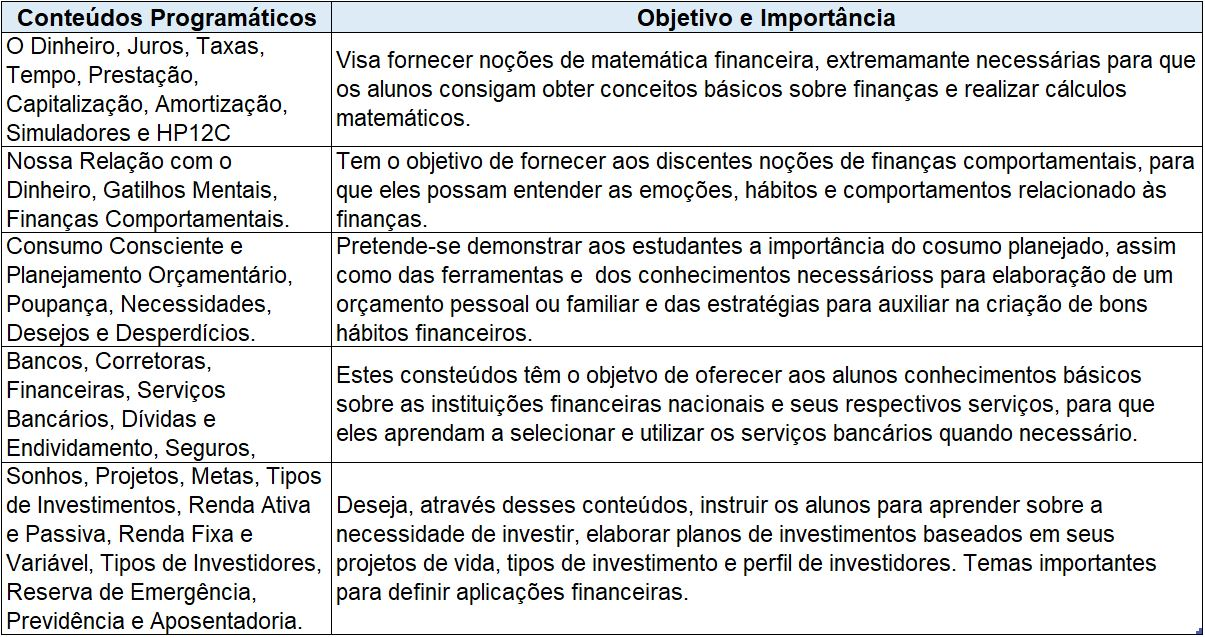
\includegraphics[width=1.0\textwidth]{quadro-04-conteudo-programatico}
\legend{\footnotesize Fonte: Do Autor}
\label{quad: quadro-04-conteudo-programatico}
\end{minipage}
\end{quadro}

A proposta de aplicação do curso “Educação Financeira através de Jogos” foi discutida entre os professores ministrantes, considerando a análise de trabalhos anteriores, referencial teórico, o público-alvo e a experiência dos docentes. Os professores consideraram que a ordem de apresentação das unidades temáticas que facilitaria o processo de ensino-aprendizagem seria a seguinte:

\begin{enumerate}
    \item Introdução à matemática financeira;
    \item Finanças comportamentais;
    \item Consumo consciente;
    \item Instituições financeiras e serviços;
    \item Investimentos e previdência. 
\end{enumerate}

A terceira etapa apresentou a oferta do curso “Educação Financeira através de Jogos” para os alunos de todas as turmas do ensino médio integrados do IFSUL-Câmpus Gravataí, por intermédio de um projeto de ensino aprovado pela Pró-reitoria de Ensino do IFSUL. O plano de aulas construído foi aplicado em 8 encontros presenciais no segundo semestre de 2019, com a participação de dezoito alunos de diversas turmas e três membros docentes ministrantes, especialistas em matemática financeira, contabilidade e investimentos, informática e educação. Devido ao fato do projeto ser voltado ao ensino médio integral, participaram do curso alunos com idades entre 15 a 19 anos, de todas as séries do ensino médio integrado do câmpus (do 1º ao 4º ano). O gráfico 1 exibe a faixa etária dos sujeitos da pesquisa que participaram do curso, nele é possível observar que a maior parte dos estudantes (44\%) possuíam 16 anos de idade no momento do curso. Em relação ao sexo dos discentes participantes 61\% eram do sexo masculino e do 39\% feminino.

\graphicspath{{graficos/}} 
\begin{grafico}[!ht]
\centering
\begin{minipage}{0.7\textwidth}
\caption{Faixa Etária do Alunos}
\centering
\includegraphics[width=0.95\textwidth]{g1-faixa-etária}
\legend{\footnotesize Fonte: Dados da Pesquisa}
\label{graf: g1-faixa-etária}
\end{minipage}
\end{grafico}

O docente especialista em matemática financeira e educação lecionou a unidade temática de introdução à matemática financeira, o professor especialista em contabilidade e investimentos lecionou a unidade temática referente à investimentos e previdência. Durante todo o processo de ensino-aprendizagem destas duas unidades os ministrantes e alunos tiveram assessoria do autor da presente proposta, pesquisador e mestrando de informática na educação, que também foi responsável por trabalhar as outras unidades temáticas com os discentes.

A infraestrutura necessária para o desenvolvimento desse projeto e execução do plano de ensino nas aulas do curso “Educação Financeira através de Jogos” para ensino médio integrado inclui:

\begin{itemize}
    \item Material impresso e digital;
    \item Material auxiliar disponibilizado na plataforma \textit{moodle};
    \item Laboratório de informática com acesso à \textit{internet};
    \item Jogos sérios digitais e de tabuleiro;
    \item Projetor multimídia;
    \item Quadro branco.
\end{itemize}

O conteúdo do curso foi ministrado através de exposições orais e aulas práticas com atividades no laboratório de informática e/ou trabalhos escritos de cálculos e planejamento, direcionados para a resolução de problemas e exercícios práticos de finanças pessoais e investimentos, visando fixar o conteúdo abordado, com auxílio de tecnologias educacionais como jogos, simuladores e ambientes virtuais de aprendizagem. Acredita-se que buscar novas formas de transmitir o conhecimento em sala de aula é relevante, principalmente quando os novos meios de interação que surgem influenciam as formas de pensar e, consequentemente, os estilos de aprendizagem dos estudantes \cite{prensky2012}. Nesse sentido, os jogos sérios podem ser usados no processo de ensino-aprendizagem, pois são desenvolvidos para serem cativantes ao mesmo tempo em que se propõem a alcançar algum objetivo pedagógico.

Na quarta etapa ocorreu a aplicação dos questionários do método avaliativo MEEGA+ (\textit{Model for Evaluating Educational Games}, em português Modelo para Avaliação de Jogos Educativos) para avaliar a percepção de aprendizagem dos alunos utilizando os jogos, dos questionários de aprendizagem, de avaliação do curso e de avaliação de aplicação do conhecimento adquirido pelos alunos. Os instrumentos avaliativos permitiram ao pesquisador coletar dados para a derradeira etapa da pesquisa na qual realizou-se a análise das informações e a produção dos resultados do presente trabalho.

A presente pesquisa tem uma abordagem qualitativa ao analisar os dados obtidos, os quais serão recolhidos por intermédio das respostas dos estudantes nos questionários constantes nos apêndices A, B e C, bem como pelo método avaliativo de jogos MEEGA+, segundo Minayo (\citeyear{minayo2008}) a pesquisa qualitativa possibilita reorganizar relações, procedimentos, símbolos e acepções da realidade social, no caso do presente trabalho reorganizar as relações financeiras dos sujeitos.

A educação financeira é um conteúdo relativamente recente no ensino médio \cite{souza-flores2018} e também na RFEPCT, ainda não estabelecido, portanto, quanto aos objetivos a presente pesquisa classifica-se como exploratória e em relação à sua natureza como aplicada, pois utiliza-se de conhecimentos adquiridos por meio de pesquisas bases anteriores para resolver um problema específico, que é a falta de educação financeira no ensino médio integrado da RFEPCT.

\section{CAMPO DA PESQUISA}
Como informado em capítulos anteriores a pesquisa deste estudo será aplicada no IFSUL-Câmpus Gravataí, inaugurado em 2014 na respectiva cidade, entretanto este processo educacional começou há anos no estado. A história da educação profissional federal no Rio Grande do Sul teve início em 1930 quando foi inaugurado a primitiva Escola de Aprendizes e Artífices, a primeira escola federal do estado voltada ao ensino profissional. Assim como as outras escolas desta modalidade, a unidade do Rio Grande do Sul também sofreu e promoveu alterações políticas nos cursos oferecidos, no público atendido e na sua nomenclatura, e por intermédio da Lei Nº 11.892, em 29 dezembro de 2008, tornou-se o Instituto Federal de Educação, Ciência e Tecnologia Sul-rio-grandense - IFSUL \cite{ifsul2015}. Atualmente este instituto possui cursos técnicos (integrados, concomitante e subsequente), de graduação (licenciatura, bacharelado e tecnologia), de pós-graduação lato sensu e stricto sensu (mestrado e doutorado), em diversas áreas do conhecimento, distribuídos em 14 campi localizados nas cidades de Bagé, Camaquã, Charqueadas, Gravataí, Jaguarão, Lajeado, Avançado Novo Hamburgo, Passo Fundo, Santana do Livramento, Sapiranga, Sapucaia do Sul, Venâncio Aires e Pelotas.

O Campus Gravataí iniciou as atividades no segundo semestre de 2014, com o curso Técnico Subsequente de Informática. Atualmente o campus possui cinco cursos: Pós-graduação em Educação Física Escolar, as Graduações em Análise e Desenvolvimento de Sistemas e em Formação Pedagógica para Graduados não Licenciados, o Técnico de Informática (subsequente) e o Técnico de Informática para Internet (integrado ao ensino médio) no qual foi aplicada a pesquisa do presente estudo.

Pela natureza e vocação do IFSUL, as diversas teorias educacionais e metodologias de ensino podem ser exploradas para dar suporte efetivo à formação do futuro profissional dos alunos do Câmpus Gravataí, inclusive na construção do conhecimento da educação financeira com apoio de tecnologias educacionais e epistemologias fundamentadas.

\section{OS JOGOS UTILIZADOS}
Durante a pesquisa exploratória sobre jogos sérios e de entretenimento que podem ser utilizados no processo de ensino-aprendizagem de educação financeira para jovens encontrou-se diversos jogo de tabuleiro como o Desafios Financeiros, \textit{Monopoly}, Banco Imobiliário, Jogo da Vida, Jogo da Mesada, Piquenique, \textit{Cash-flow}, Bons Negócios, Administrando o seu Dinheiro, Catan, Renda Passiva e jogos digitais como o \textit{Cash-flow}, \textit{SimCity}, \textit{The Sims}, \textit{Animal Crossing}, Bate-bola Financeiro, \textit{League of Legends}, \textit{Money Race} 2, Tá O\$\$O, Jogo Vida Financeira, \textit{Tycoon City: New York} e Investindo na Vida.

Foram escolhidos dois jogos para serem utilizados como apoio à aprendizagem dos discentes durante as aulas no curso educação financeira para jovens, o protótipo Orçamento Consciente e o Renda Passiva. Esses jogos foram escolhidos, pois, permitem ao aluno o aprendizado através de erros e a elaboração de soluções, incentivando-os a resolver problemas financeiros de um modo lúdico, refletindo sobre os resultados e os processos de elaboração das soluções, até encontrar um ou mais métodos de soluções possíveis. Ademais, o jogo Orçamento Consciente foi escolhido por trabalhar diretamente com finanças comportamentais e orçamento financeiro. Durante a pesquisa não se encontrou jogos sérios e trabalhos acadêmicos relacionados ao ensino de finanças comportamentais em orçamento financeiro para jovens por meio de jogos educativos. Por isso, houve a necessidade de desenvolver o protótipo do jogo Orçamento Consciente para utilizá-lo durante as aulas do curso, o jogo trabalha os aspectos da economia comportamental elaborados por Kahneman (\citeyear{kahneman2012}).

Para mais, normalmente nos jogos de educação financeira do tipo tabuleiro como o \textit{Monopoly}, \textit{Cash-flow} e Banco Imobiliário os jogadores percorrem um caminho semelhante para solucionar os problemas, alcançar os objetivos e ganhar o jogo, dependendo principalmente da sorte para isto. Entretanto, no jogo Renda Passiva, assim como na vida financeira real, não existe um caminho único para solucionar os problemas, alcançar os objetivos e lograr êxito, dessa forma o jogo permite aos jogadores elaborarem diversas soluções distintas, aprendendo com os próprios erros e acertos adquirindo assim o conhecimento. O Jogo Renda Passiva é um jogo de regras sobre finanças pessoais e familiar, diferente dos jogos tradicionais de tabuleiro onde a sorte é condição principal para ganhar, no Renda Passiva os jogadores deverão desenvolver a capacidade de resolver problemas financeiros para ganhar o jogo \cite{frechiani2019a}, de uma forma lúdica, divertida e inteligente pode-se aprender conceitos da educação financeira através do jogo sério, o conteúdo a ser ensinado aos alunos fazem parte da regra do jogos, fato que facilita a aprendizado.

Os fatores descritos nos parágrafos anteriores foram decisivos na escolha dos jogos utilizados no processo de ensino-aprendizagem durante o curso, contudo é importante descrever motivos para exclusão de outros. Dos jogos encontrados excluíram-se os que não permitiam a interação entre os alunos, que o fator de sorte é componente decisivo na jogabilidade, que trabalham com poucos conteúdos das unidades temáticas, que lidam apenas com perguntas e respostas, que o público-alvo são crianças e com custo elevado para aquisição, pois nem sempre a instituição de ensino possui recursos para compra de jogos, deste modo quanto menor o custo relacionado melhor. Os aspectos inerentes aos jogos escolhidos, assim como o uso destes nos processos educativos estão descritos neste capítulo nos próximos itens.

\subsection{O Jogo Orçamento Consciente}
O jogo Orçamento Consciente é um protótipo de um jogo sério digital multiplataforma, disponível para computadores e \textit{smartphones}, desenvolvido em 2018 pelos alunos Camila Peres, Johnata Santicioli (autor da presente proposta) e Willian Chimura alunos do Mestrado Profissional em Informática na Educação no Instituto Federal do Rio Grande do Sul.

O jogo simula o recebimento de um salário mensal de R\$3.000,00 que deve ser dividido em três necessidades (categorias de despesas): compras e conforto, alimentação e saúde nesta ordem da esquerda à direita conforme a figura \ref{fig: figura01-salario}, neste momento inicial ilustrado na imagem, o jogador realiza um orçamento financeiro mesmo que de forma não planejada, após distribuir todo o salário do mês o jogo apresenta uma contagem regressiva para início do jogo, figura \ref{fig: figura02-contagem}.

\graphicspath{{figuras/}}
\begin{figure}[!ht]
\centering
\begin{minipage}{1.\linewidth}
\center
\caption{Jogo Orçamento Consciente (Distribuição do Salário)} \label{fig: figura01-salario}
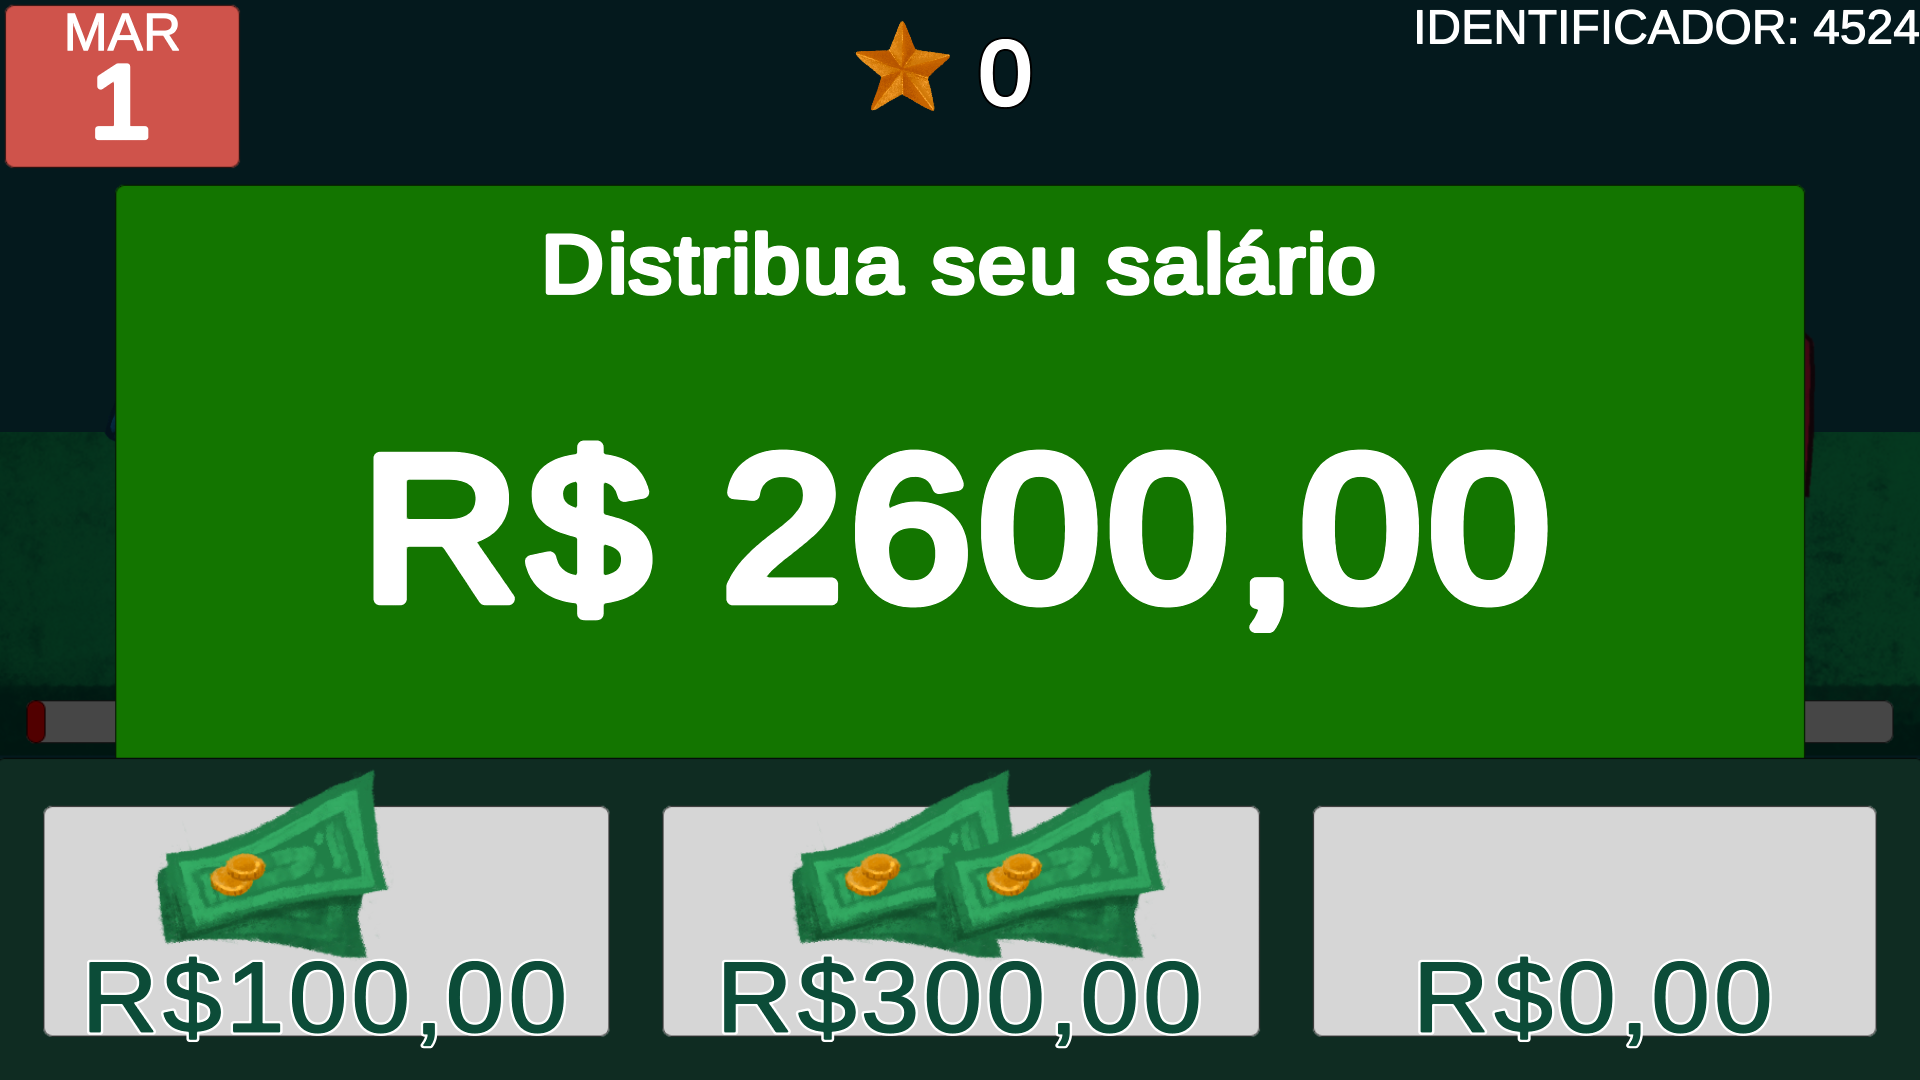
\includegraphics[width=0.4\linewidth]{01-figura_distribuicao-salario.png}
\legend{\footnotesize Fonte: Dos Autores}
\end{minipage}
\end{figure}

\graphicspath{{figuras/}}
\begin{figure}[!ht]
\centering
\begin{minipage}{1.\linewidth}
\center
\caption{Jogo Orçamento Consciente (Contagem Regressiva)} \label{fig: figura02-contagem}
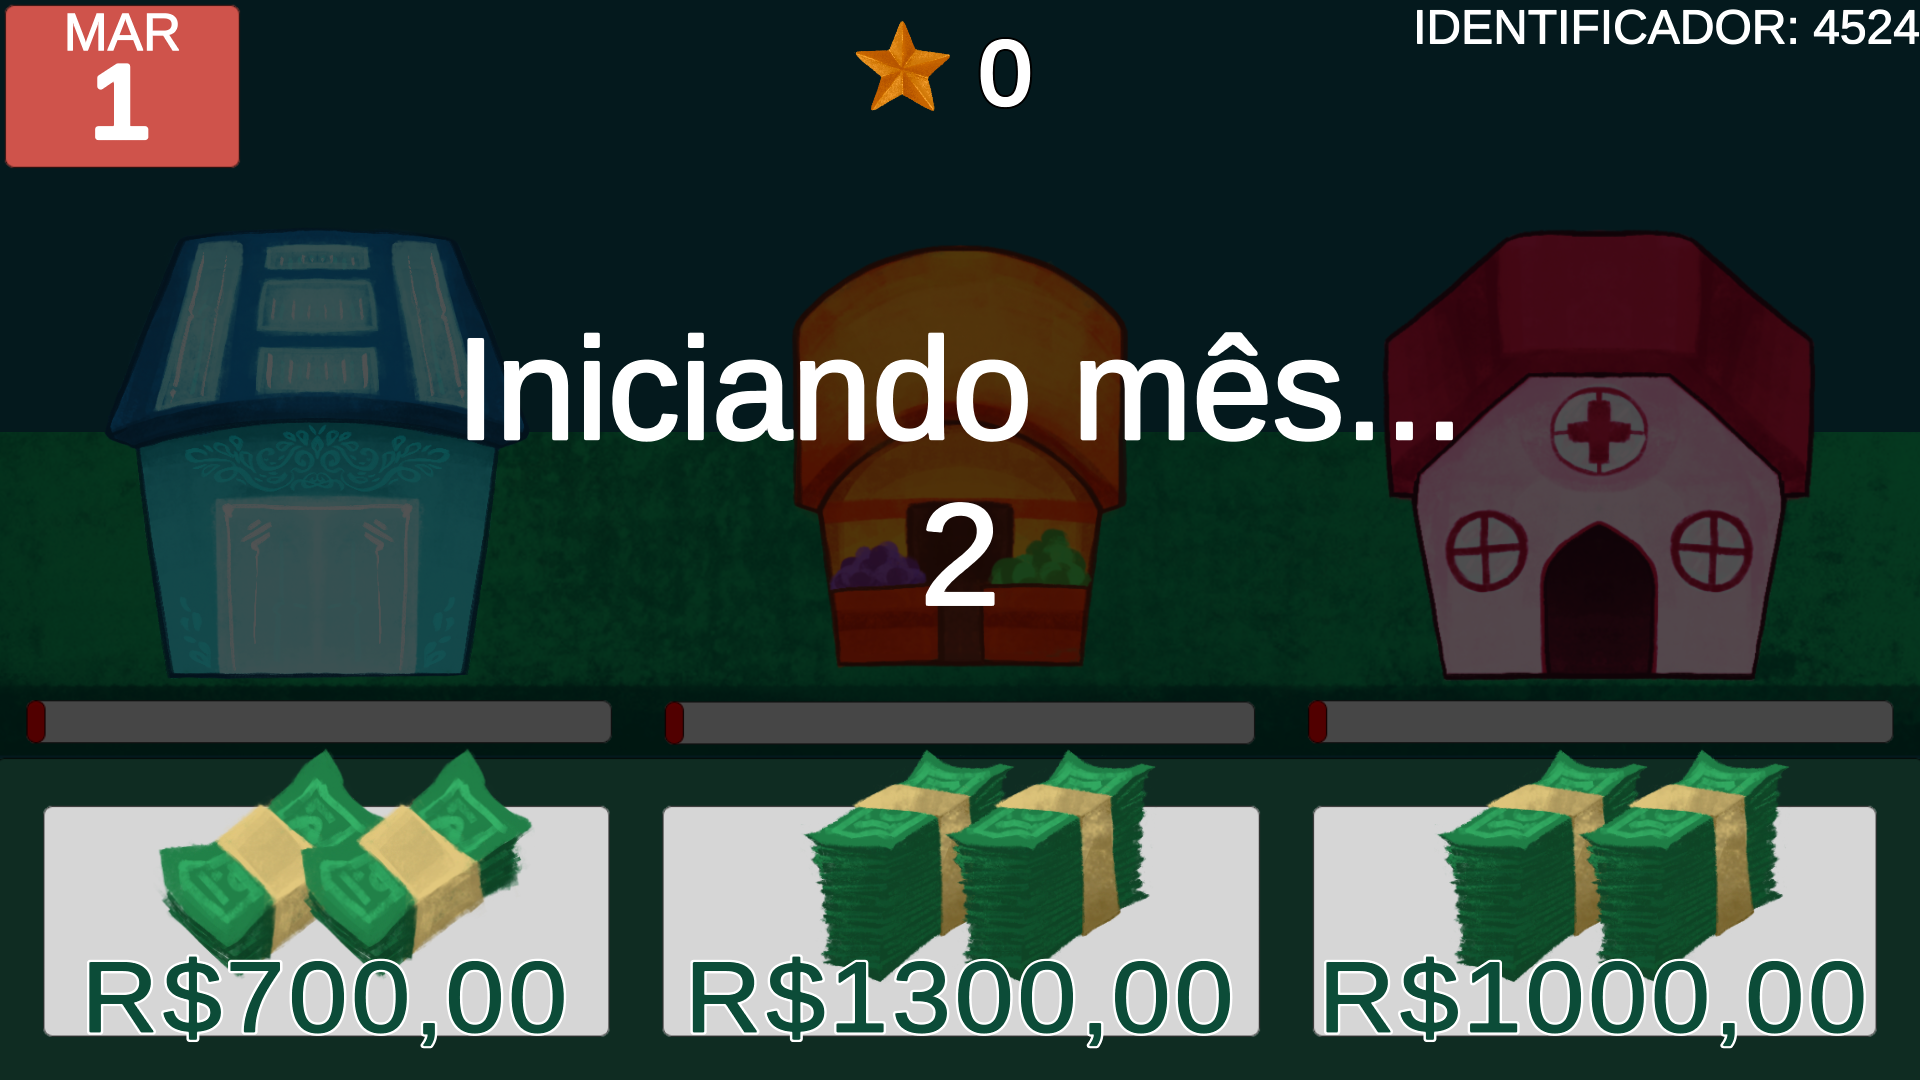
\includegraphics[width=0.4\linewidth]{02-figura_contagem-regressiva-mes.png}
\legend{\footnotesize Fonte: Dos Autores}
\end{minipage}
\end{figure}

\newpage
Ao longo de “um mês”, que dentro do jogo dura aproximadamente 1 minuto, o jogador deve equilibrar suas necessidades, escolhendo quais produtos comprar e quais ignorar, considerando o custo-benefício e seu planejamento inicial (figura \ref{fig: figura03-mercado} e \ref{fig: figura04-shopping}), podendo apenas utilizar o dinheiro da necessidade com o respectivo produto, em outras palavras, utilizar o dinheiro reservado para saúde apenas com produtos de saúde. O jogador não pode transferir dinheiro de uma necessidade para outra, ao esgotar os recursos destinados para determinada necessidade, o jogador precisa esperar até o mês seguinte para repensar sua estratégia e ajustar o planejamento orçamentário para torná-lo superavitário ou neutro.

\graphicspath{{figuras/}}
\begin{figure}[!ht]
\centering
\begin{minipage}{1\linewidth}
\centering
\caption{Jogo Orçamento Consciente (Produto Mercado)} \label{fig: figura03-mercado}
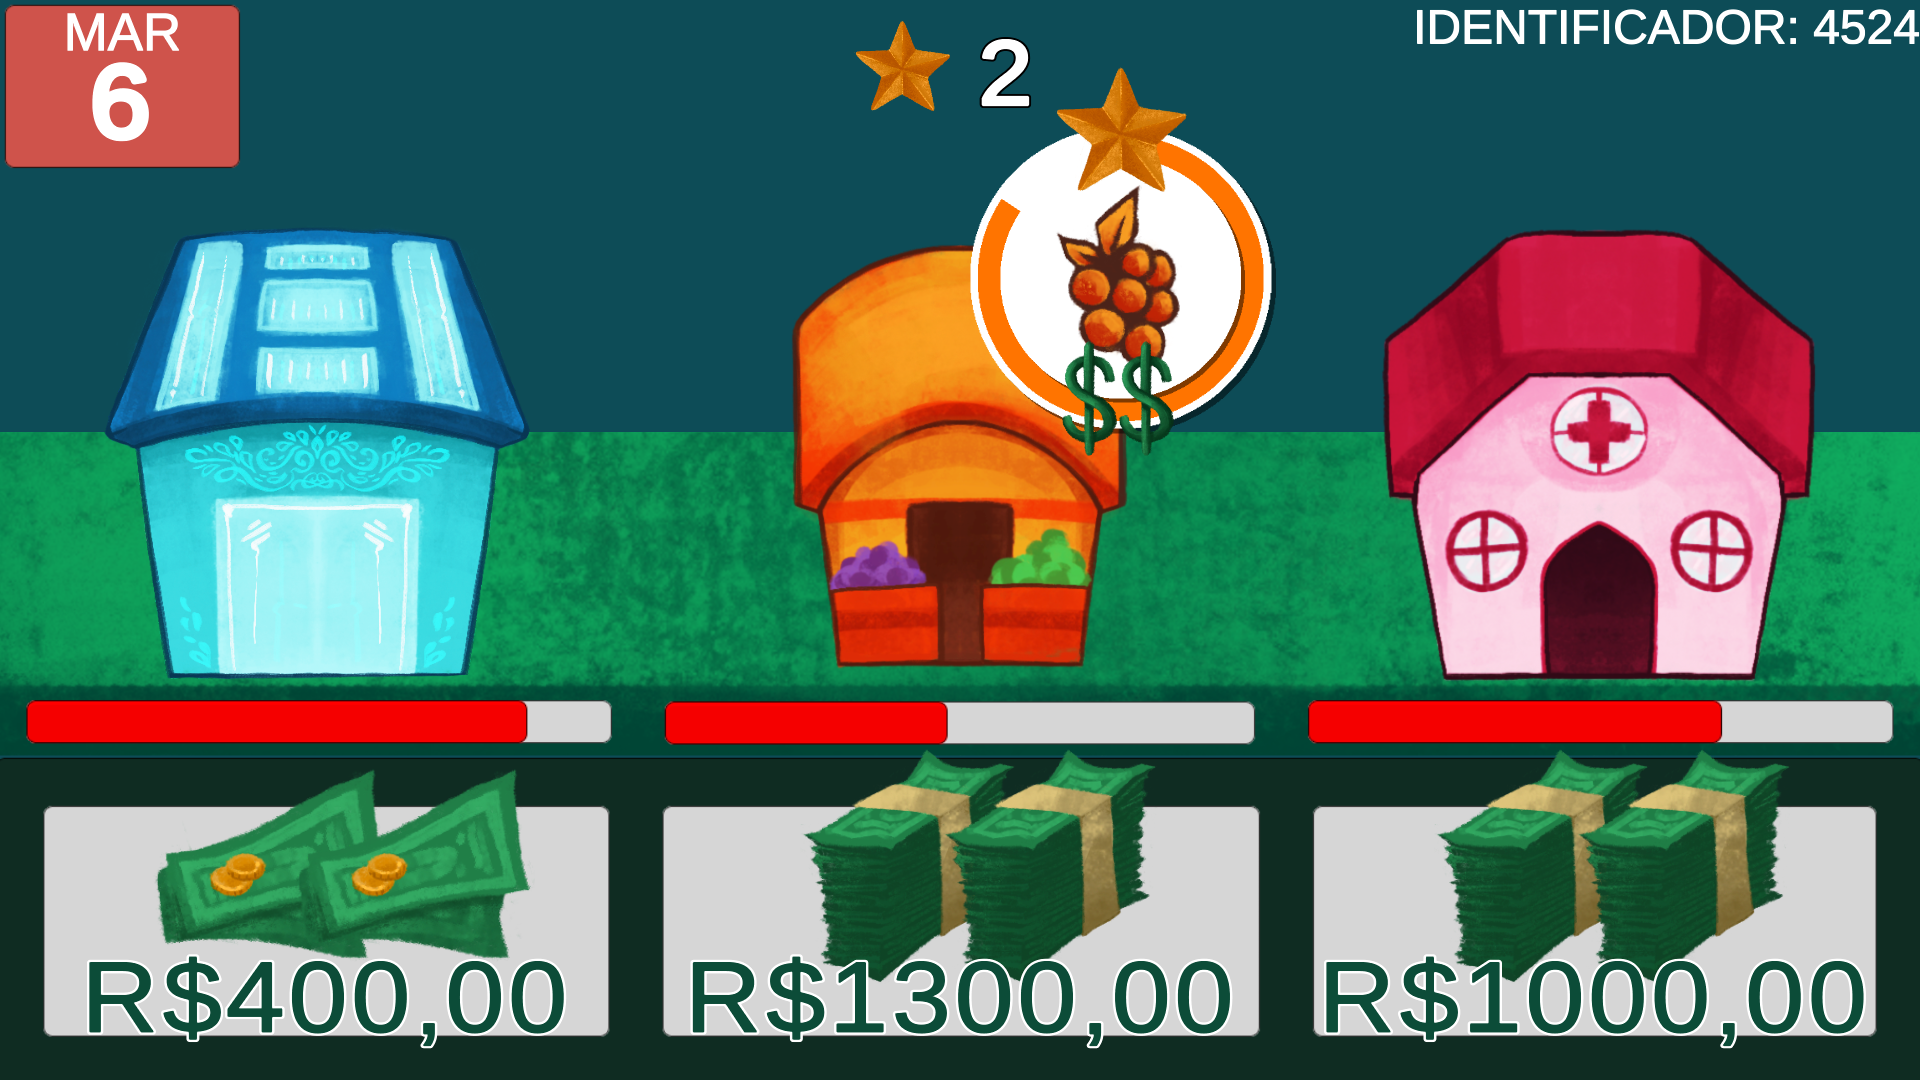
\includegraphics[width=0.4\linewidth]{03-figura_tela-jogo-mercado.png}
\legend{\footnotesize Fonte: Dos Autores}
\end{minipage}
\end{figure}

\graphicspath{{figuras/}}
\begin{figure}[!ht]
\centering
\begin{minipage}{1\linewidth}
\centering
\caption{Jogo Orçamento Consciente (Produto Shopping)} \label{fig: figura04-shopping}
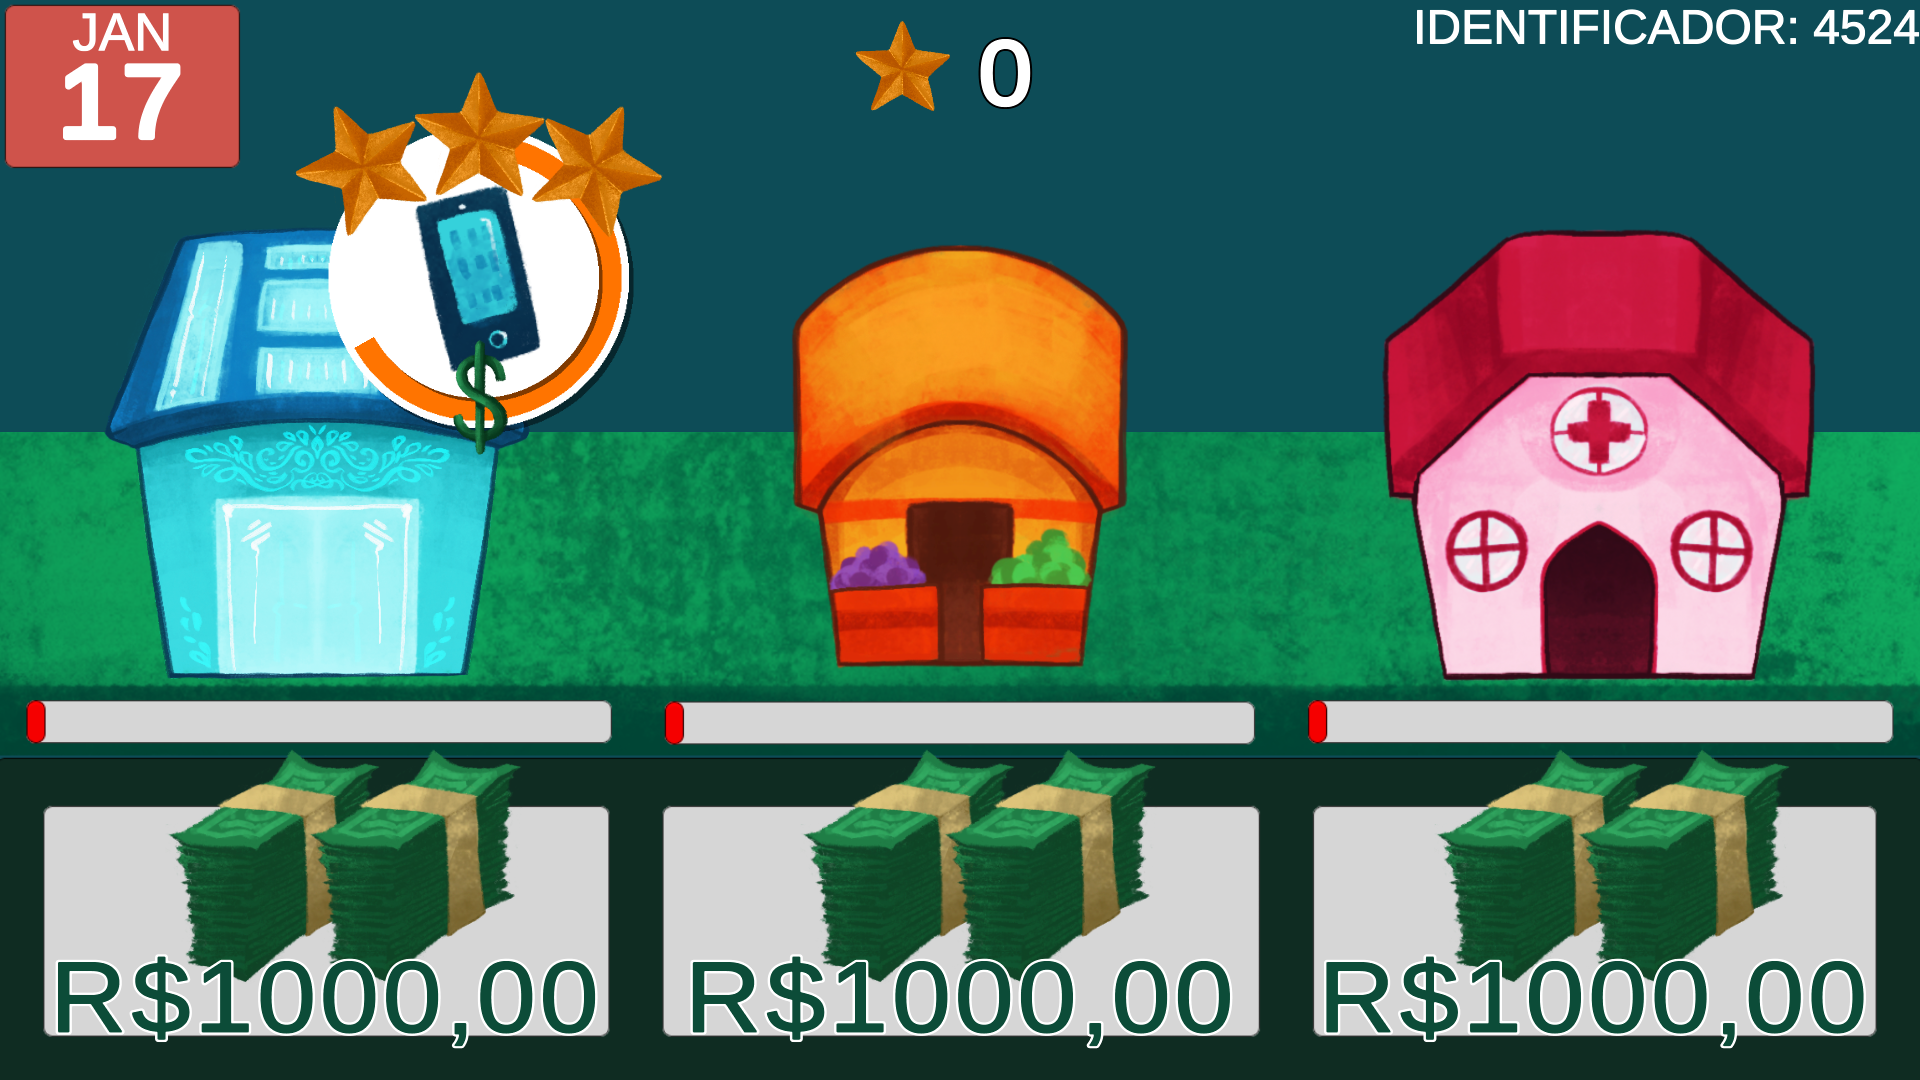
\includegraphics[width=0.4\linewidth]{04-figura_tela-jogo-shopping.png}
\legend{\footnotesize Fonte: Dos Autores}
\end{minipage}
\end{figure}

A tela principal do jogo, exibidas nas figuras \ref{fig: figura03-mercado} e \ref{fig: figura04-shopping}, apresenta três “prédios" (construções do jogo), um azul que representa um shopping, relacionado à “necessidade de compras e conforto”, um mercado na cor laranja, que corresponde a “necessidade de alimentação” e uma farmácia rosa simbolizando a “necessidade de remédios ou saúde”. As barras horizontais vermelhas (“barras de necessidade”) embaixo de cada construção indicam ao jogador a necessidade de consumir produtos de acordo com sua categoria. Essas barras iniciam totalmente preenchidas (necessidade de consumo atendida) e diminuem conforme o tempo do jogo, representando o dever de uma nova compra. Abaixo de cada uma das barras encontra-se a quantidade de dinheiro distribuída no começo de cada mês do jogo e disponível para o consumo da respectiva necessidade.

Cada “prédio” oferece opções de produtos relativos à necessidade que representa, um após o outro, cabendo ao jogador a decisão de comprar ou não os produtos disponíveis. Para efetuar a compra o jogador deve selecionar o produto, considerando o planejamento orçamentário realizado, se o item é necessário e se é viável a sua aquisição. Cada produto possui diferentes níveis de qualidade, representados por estrelas (de uma a três), assim como diferentes preços, caracterizados por cifrões (de um a três) cada um equivalente a cem reais. Quanto maior a qualidade do produto, maior será a quantidade de estrelas e supre mais a necessidade de consumo, aumentando o preenchimento da barra vermelha que indica a necessidade. Por exemplo, a figura \ref{fig: figura03-mercado} ilustra um item que pode ser comprado pelo o jogador junto ao prédio do supermercado, um cacho uva que possui qualidade nível 1, pois tem uma estrela, e preço de R\$ 200 (duzentos reais), porque há 2 (dois) cifrões. Cada item comprado faz com que o orçamento planejado sofra alterações, diminuindo os recursos para a aquisição de itens de uma mesma categoria. Os produtos ficam disponíveis para compra por um determinado tempo, controlado pelo círculo laranja em volta do produto, quando o círculo completa uma volta o tempo para comprar o produto acaba (uso dos Gatilhos Mentais da Urgência e Escassez) e então desaparece e eventualmente são substituídos por outros, com diferentes qualidades e preços. Nas figuras \ref{fig: figura03-mercado} e \ref{fig: figura04-shopping}, acima das construções existe um contador de estrelas, referente à qualidade do produto, ao comprar produtos de maior qualidade essa pontuação aumenta conforme a quantidade de estrelas do produto. Ao esvaziar completamente a barra de necessidade, essa ficará cinza, pois não houve consumo suficiente, cabe ao jogador impedir que a barra fique totalmente cinza escolhendo quais produtos comprar, baseando-se em seu planejamento inicial, preço, qualidade e necessidade.

Ao final do mês o jogador recebe um relatório detalhando as necessidades que foram atendidas ou não e sua pontuação (figuras \ref{fig: figura05-relatorio-01} e \ref{fig: figura06-relatorio-02}), a cada dia que uma das barras de necessidade estiver totalmente vazia (cinza) é descontada uma estrela do total, em caso de sobra de recursos, cada R\$ 100 é convertido em uma estrela. Por exemplo, na figura \ref{fig: figura06-relatorio-02}, o relatório mês indica que o jogador passou 4 dias sem recurso no Shopping, 3 dias sem recursos no Mercado e poupou com R\$ 500 de seu salário, neste caso o jogador deverá perder 7 estrelas (pelos dias de necessidades não atendidos) e ganhar 5 estrelas (pelo dinheiro poupado), como resultado duas estrelas serão retiradas das 56 que ele possui.

\graphicspath{{figuras/}}
\begin{figure}[!ht]
\centering
\begin{minipage}{1\linewidth}
\center
\caption{Jogo Orçamento Consciente (Tela de Relatório Mês 1)} \label{fig: figura05-relatorio-01}
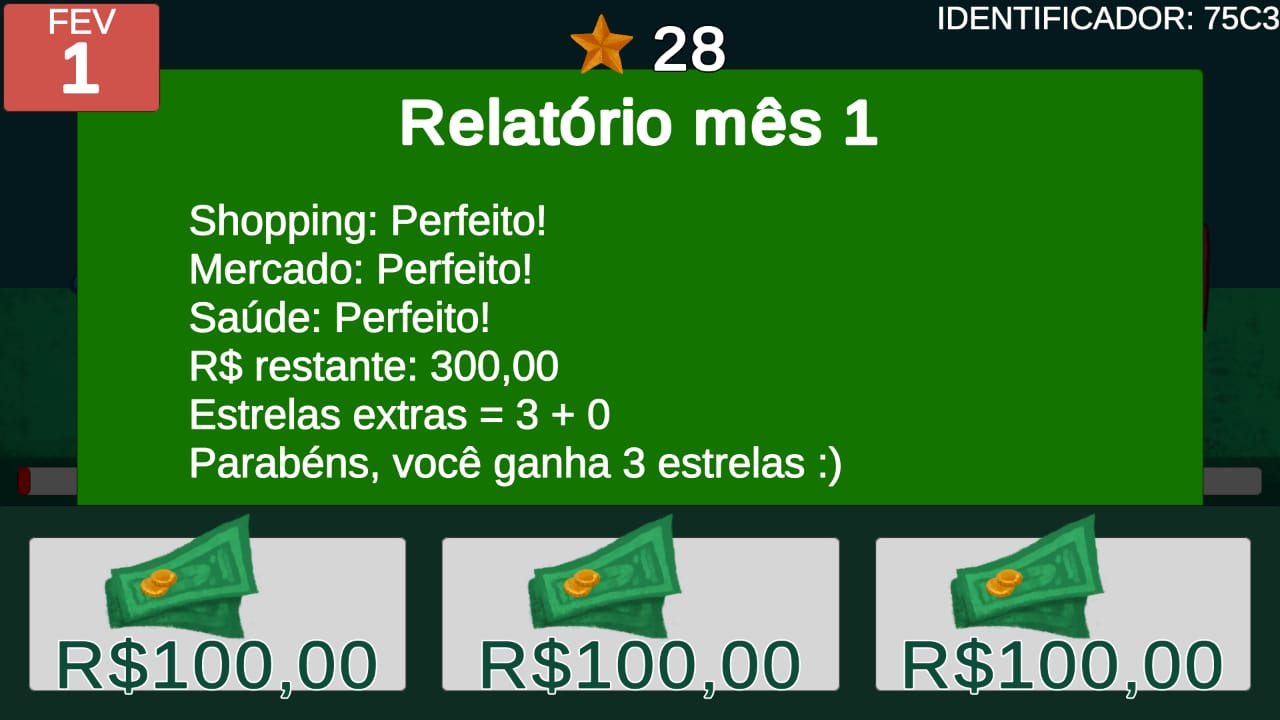
\includegraphics[width=0.4\linewidth]{05-figura_relatorio-mes-1}
\legend{\footnotesize Fonte: Dos Autores}
\end{minipage}
\end{figure}

\graphicspath{{figuras/}}
\begin{figure}[!ht]
\centering
\begin{minipage}{1\linewidth}
\center
\caption{Jogo Orçamento Consciente (Tela de Relatório Mês 2)} \label{fig: figura06-relatorio-02}
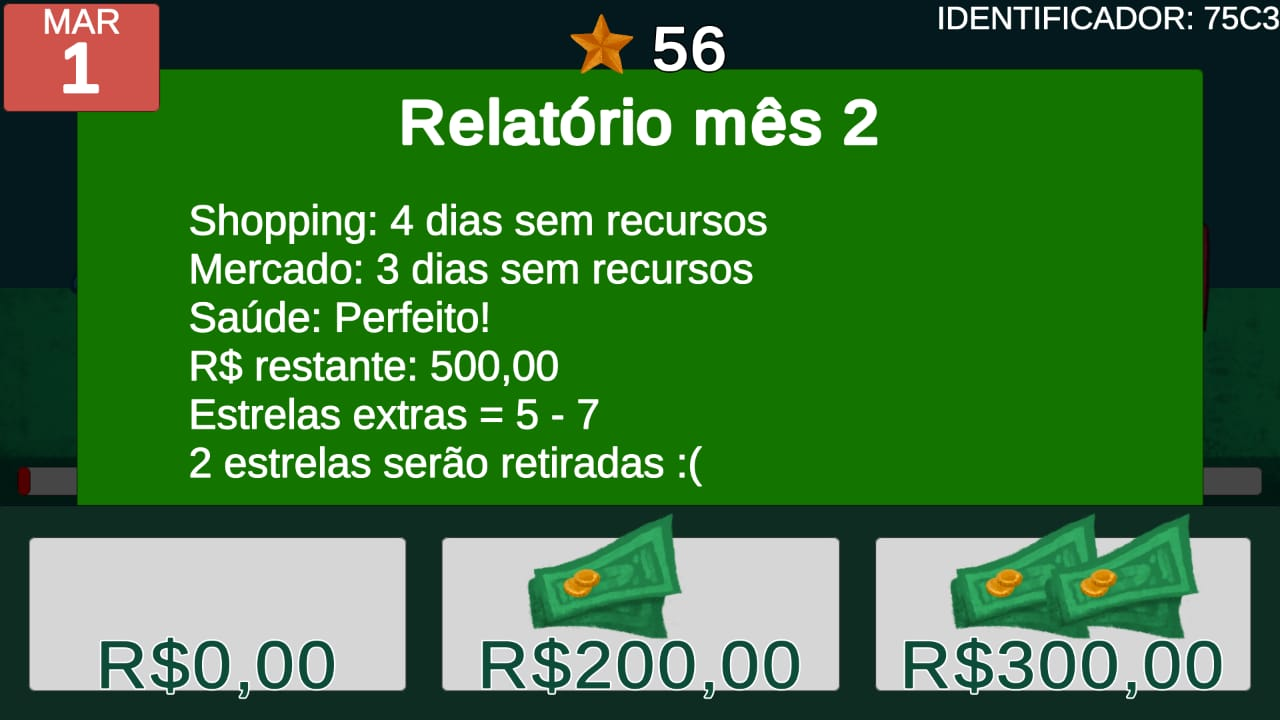
\includegraphics[width=0.4\linewidth]{06-figura_tela-relatorio-mes-2}
\legend{\footnotesize Fonte: Dos Autores}
\end{minipage}
\end{figure}

Durante o curso “Educação Financeira através de Jogos” o Orçamento Consciente foi utilizado individual pelos alunos através de computadores, para que cada aluno pudesse perceber os erros e acertos em suas tomadas de decisões financeiras durante o jogo, dessa forma, permitindo aos alunos a possibilidade de testar os conhecimentos teóricos em uma simulação simples, podendo ver as consequências de suas ações de forma rápida em um ambiente seguro.

\subsection{O Jogo Renda Passiva}
O Renda Passiva é um jogo de entretenimento, utilizado neste trabalho com intuito de um jogo sério, desenvolvido por Daniel Frechiani, simula a vida financeira pessoal e familiar, por meio de um personagem no jogo escolhido pelos jogadores, entre os seis disponíveis: microempresário, servidor público, empresário, motorista de aplicativo, professora e advogada. São utilizados peões, com imagens, para representar e movimentar os personagens escolhidos nas casas dentro do tabuleiro. Todos os personagens possuem receitas (salário ou pró-labore), gastos (fixos, variáveis, impostos, seguros, financiamento, cartão de crédito e diversos) e dívidas. No decorrer do jogo os jogadores podem contratar outros passivos financeiros e/ou obter ativos (ações, imóveis, pequenos negócios, títulos de renda fixa e ofertas dos ativos) adicionando assim uma renda passiva em seu orçamento caso tenha adquirido ativos financeiros e/ou aumentado os gastos conforme a aquisição os passivos financeiros. O controle e anotações do orçamento de cada personagem devem ser feitos por meio da ficha financeira, apresentada na figura \ref{fig: figura07-ficha-financeira}. Além das fichas financeiras o jogo possui cartas para obter negócios, imóveis, renda fixa, ofertas de venda, ações e cartas surpresas, bem como, dados para percorrer as casas, canetas e apagadores para atualizar as fichas financeiras.

\graphicspath{{figuras/}}
\begin{figure}[!ht]
\centering
\begin{minipage}{1.\textwidth}
\caption{Jogo Renda Passiva (Ficha Financeira)}
\centering
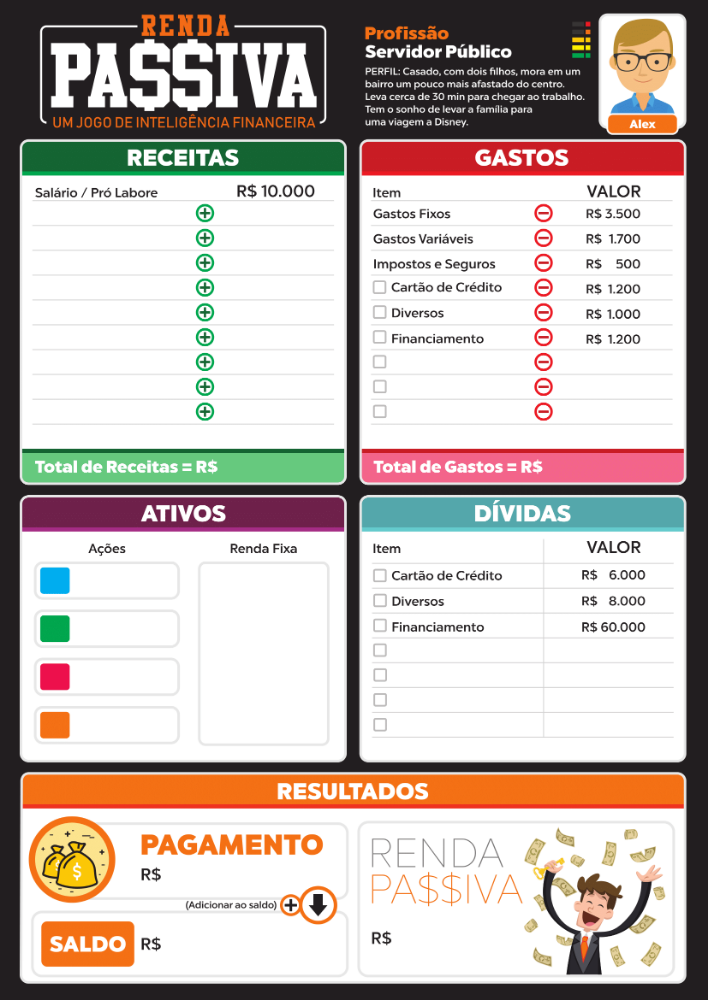
\includegraphics[width=0.45\textwidth]{07-figura_ficha-financeira-renda-passiva}
\legend{\footnotesize Fonte: Frechiane, Manual do Jogo (\citeyear{frechiani2019b})}
\label{fig: figura07-ficha-financeira}
\end{minipage}
\end{figure}

A figura \ref{fig: figura08-tabuleiro} apresenta o tabuleiro do jogo Renda passiva, o qual possui casas para movimentação dos personagens dos jogadores, 4 ações (APPL3, VAL3, BB4S, AMZ4), 1 cenário para conquista da liberdade financeira e 6 para retirar as cartas do jogo, exceto as cartas surpresa e variação que não estão localizadas nos cenários. A imagem e o significado de cada casa que o tabuleiro possui estão descritos na figura \ref{fig: figura09-cenario-jogo}, bem com os \textit{pins} dos cenários nas cores azul, cinza, amarelo e verde.
O personagem de cada jogador deve iniciar no ícone representado por uma casa no tabuleiro e precisa passar pelos ícones de sacos de dinheiros (saquinhos amarelos, figura \ref{fig: figura08-tabuleiro} e \ref{fig: figura09-cenario-jogo}) para receber pagamentos mensais (já com o total de gastos descontados das receitas). Para percorrem o tabuleiro com o personagem, os jogadores deverão jogar os dados e andar o número de casa retirados nos dados, podendo ou não entrar nos cenários ao passar por este.

\graphicspath{{figuras/}}
\begin{figure}[!ht]
\centering
\begin{minipage}{1.\textwidth}
\caption{Jogo Renda Passiva (Tabuleiro do Jogo)}
\centering
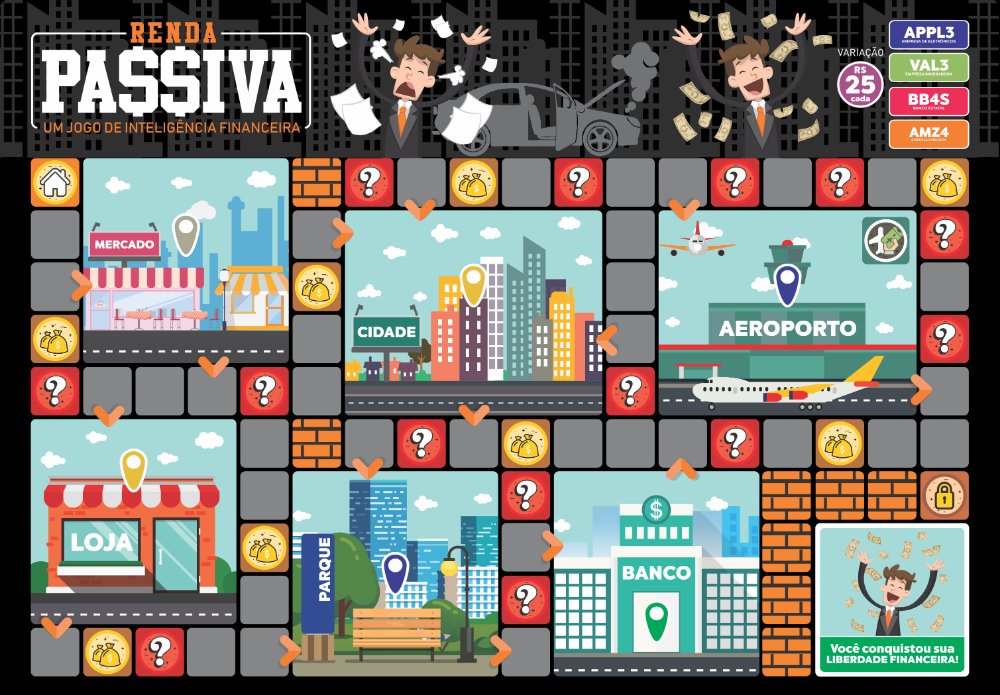
\includegraphics[width=0.5\textwidth]{08-figura_tabuleiro-renda-passiva}
\legend{\footnotesize Fonte: Frechiane, Manual do Jogo (\citeyear{frechiani2019b})}
\label{fig: figura08-tabuleiro}
\end{minipage}
\end{figure}

\graphicspath{{figuras/}}
\begin{figure}[!ht]
\centering
\begin{minipage}{0.9\textwidth}
\caption{Jogo Renda Passiva (Cenários do Jogo)}
\centering
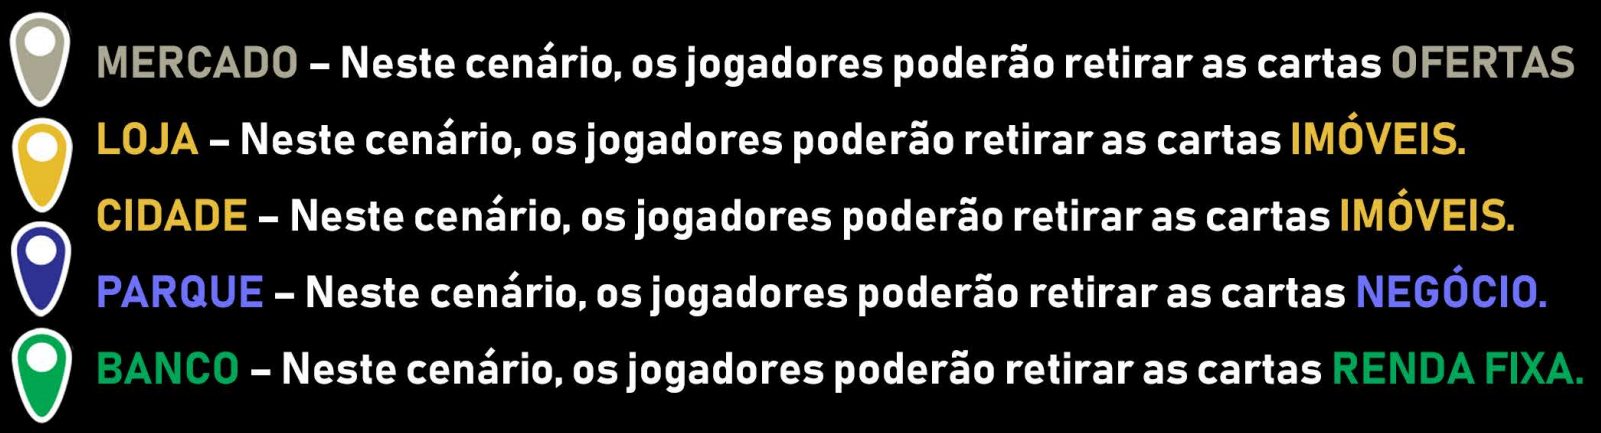
\includegraphics[width=0.8\textwidth]{09-figura_cenario-jogo-renda-passiva}
\legend{\footnotesize Fonte: Frechiane, Manual do Jogo (\citeyear{frechiani2019b})}
\label{fig: figura09-cenario-jogo}
\end{minipage}
\end{figure}

Representada pela figura \ref{fig: fig10-carta-surpresa} a carta surpresa é retirada por um jogador quando seu personagem parar na casa surpresa, representada com o ícone de interrogação na figura \ref{fig: figura08-tabuleiro} e \ref{fig: figura09-cenario-jogo}, as cartas deste tipo ocasionam imprevistos financeiros bons ou ruins como recebimento de dividendos, novos filhos, 13º salário, demissão, oportunidades de estudos para aumento do salário, bônus extra da empresa, promoção no trabalho, falência de negócios, multas de trânsito, confraternização com amigos, aquisição de material escolar, compras por impulso, restituição e pagamento de impostos. Normalmente esta carta provoca uma mudança não planejada no orçamento financeiro do personagem, obrigando o jogador a adaptar sua estratégia orçamentária. Caso ocorra um imprevisto que implique perda financeira repentina no jogo, pode-se explorar neste momento o viés comportamental de aversão a perda do ser humano para incentivar e demonstrar a importância de uma reserva financeira.

\graphicspath{{figuras/}}
\begin{figure}[!ht]
\centering
\begin{minipage}{0.8\textwidth}
\caption{Renda Passiva (Carta Surpresa)}
\centering
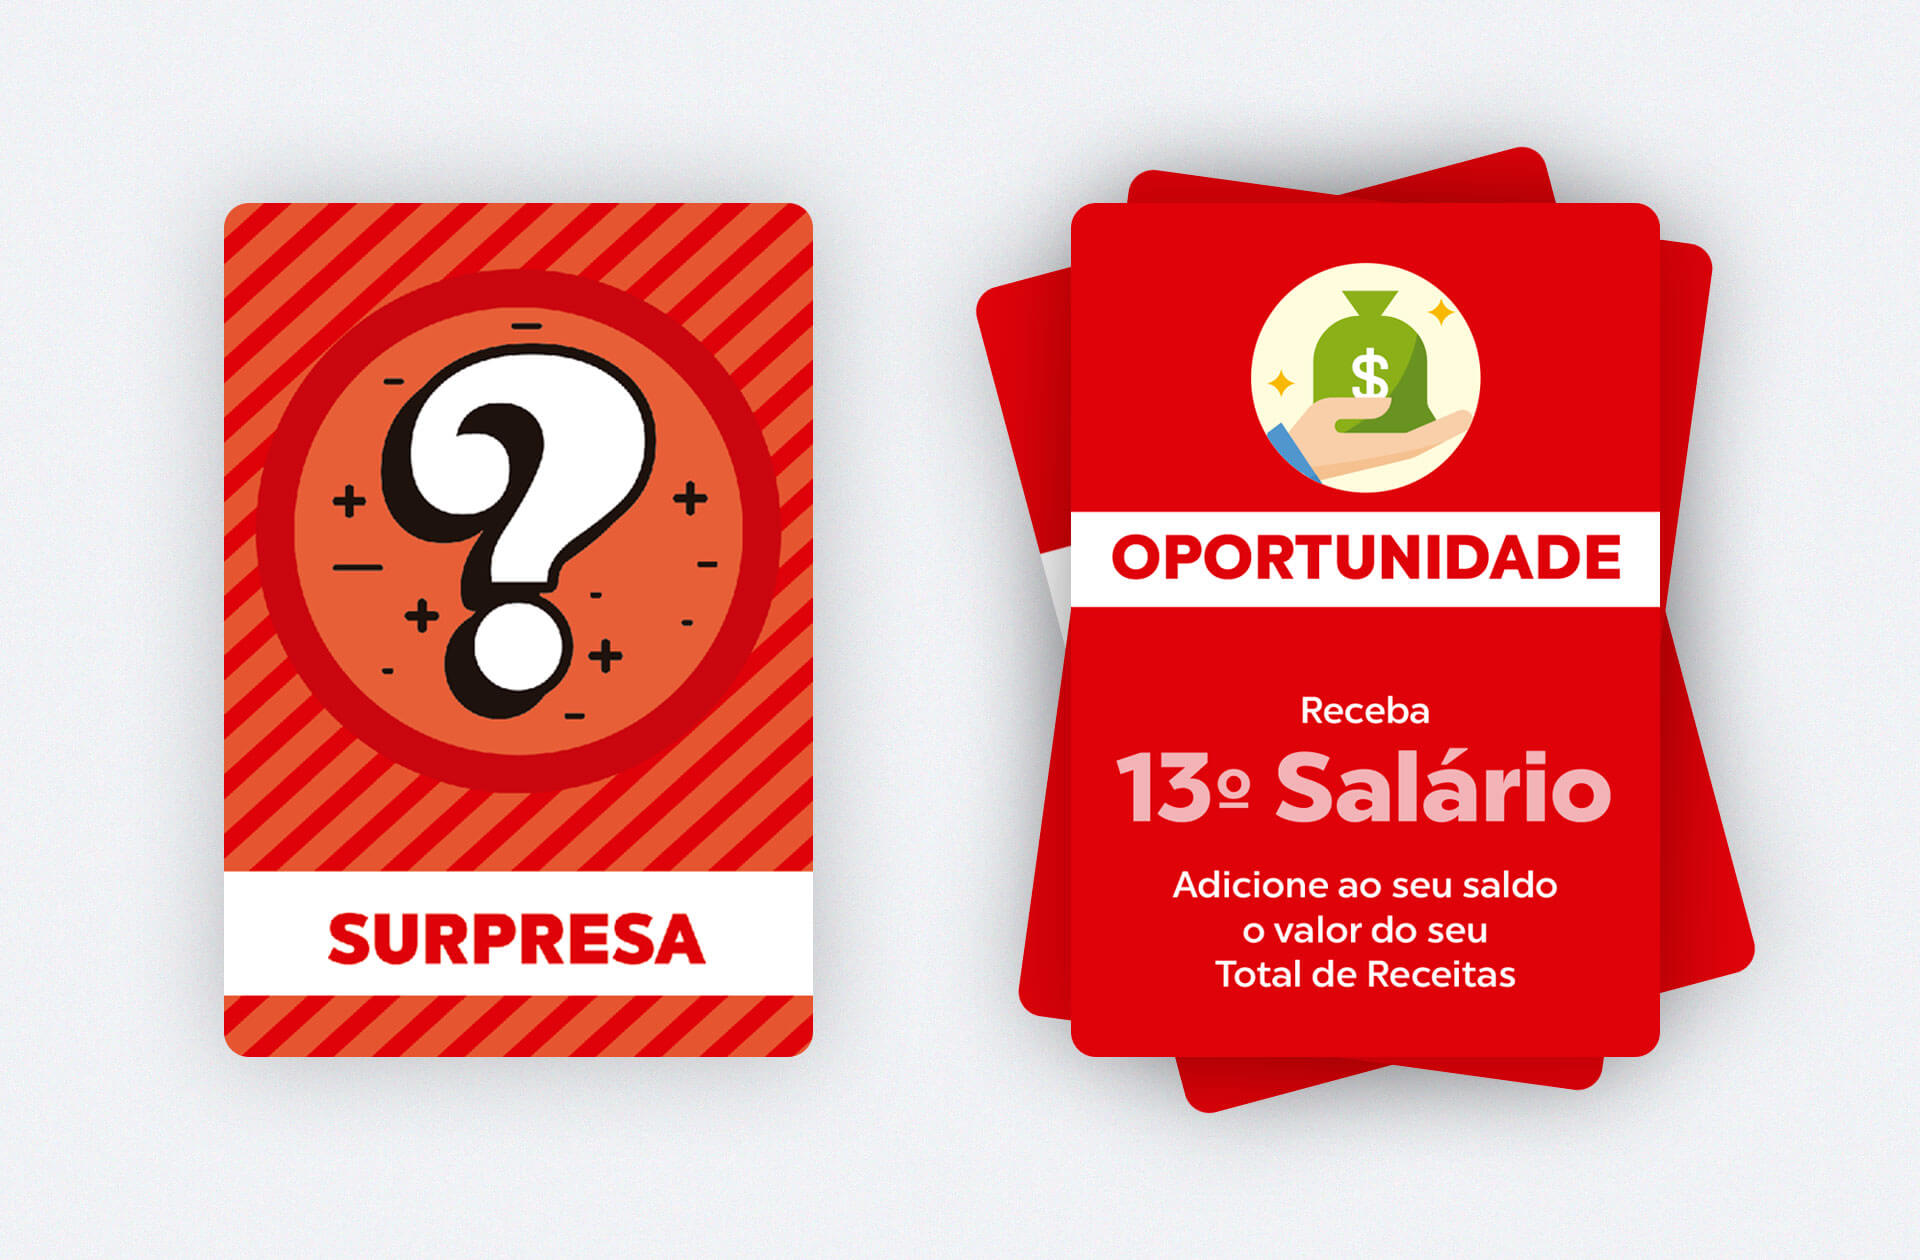
\includegraphics[width=0.8\textwidth]{figuras/fig10-carta-surpresa.jpg}
\legend{\footnotesize Fonte: Frechiane, Manual do Jogo (\citeyear{frechiani2019b})}
\label{fig: fig10-carta-surpresa}
\end{minipage}
\end{figure}

\newpage
O jogador pode retirar a carta negócio (figura \ref{fig: fig11-carta-negocio}) movendo o seu personagem até os cenários com os \textit{pins} de cor azul, aeroporto e parque (figura \ref{fig: figura08-tabuleiro}), a carta escolhida disponibiliza oportunidades para o personagem abrir algum tipo de empresa, tais como, loja de açaí, sorveteria, consertos, \textit{food truck}, barbearia, confeitaria, auto mecânica, restaurante de alimentação saudável, escola de curso EAD, hamburgueria ou um pequeno negócio, cada uma com seu respectivo aporte inicial, retorno sobre investimento e o retorno mensal.

\graphicspath{{figuras/}}
\begin{figure}[!ht]
\centering
\begin{minipage}{0.8\textwidth}
\caption{Renda Passiva (Carta Negócio)}
\centering
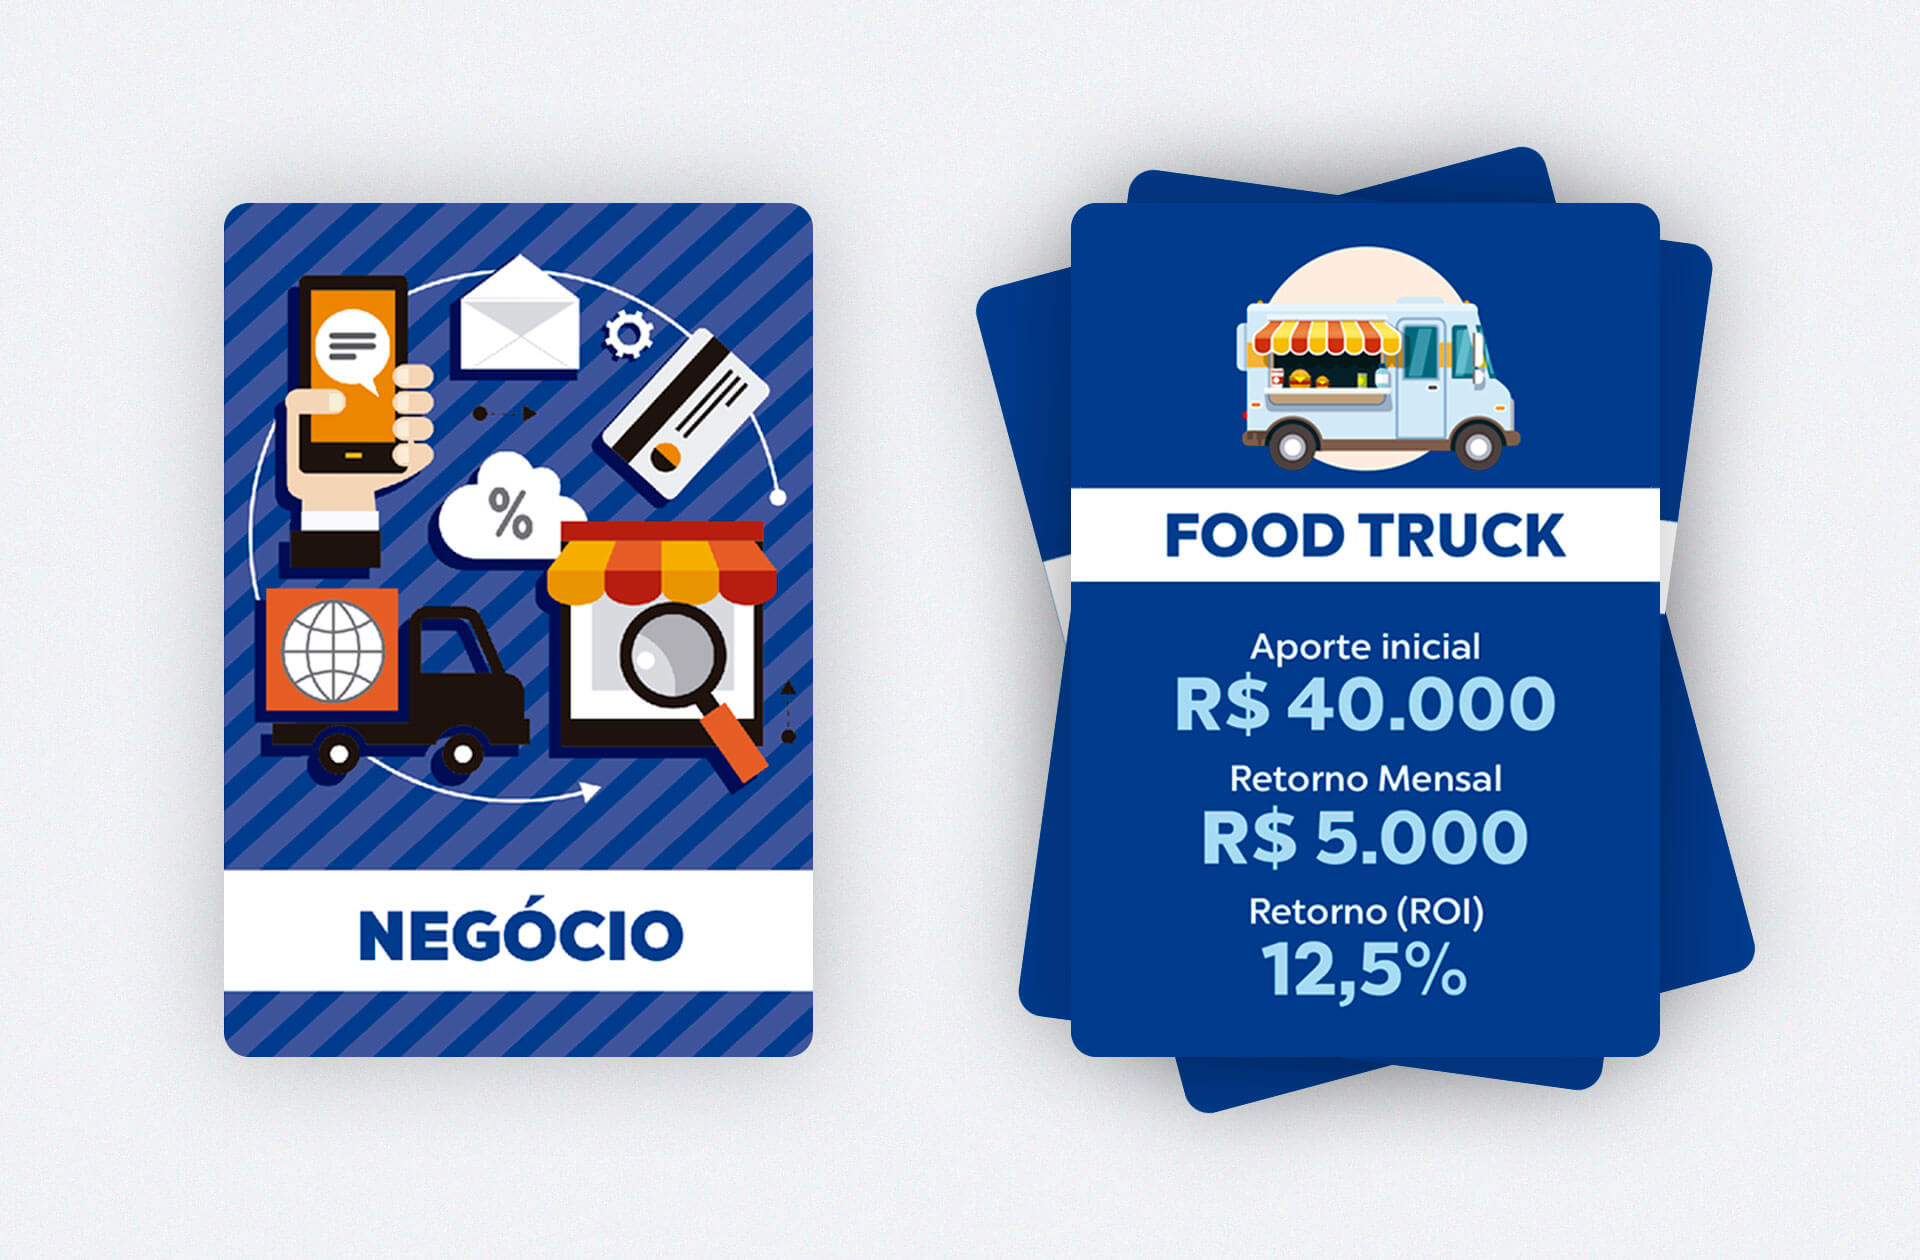
\includegraphics[width=0.8\textwidth]{figuras/fig11-carta-negocio.jpg}
\legend{\footnotesize Fonte: Frechiane, Manual do Jogo (\citeyear{frechiani2019b})}
\label{fig: fig11-carta-negocio}
\end{minipage}
\end{figure}

A figura \ref{fig: fig12-carta-imovel} apresenta exemplos da carta imóvel para retirá-la o jogador precisa deslocar seu personagem até os cenários de \textit{pins} amarelos, loja e cidade (figura \ref{fig: figura08-tabuleiro}). O jogo oferece 3 tipos de imóveis, a quitinete e os apartamento de 2 quartos ou de 4 quartos, cada imóvel possui um valor de entrada, um retorno mensal e um preço de venda. O retorno mensal de imóvel pode ser negativo representado um imóvel de aluguel que não possui um inquilino, não obtendo uma renda passiva ao personagem e aumentando suas despesas.

\graphicspath{{figuras/}}
\begin{figure}[!ht]
\centering
\begin{minipage}{0.8\textwidth}
\caption{Renda Passiva (Carta Imóvel)}
\centering
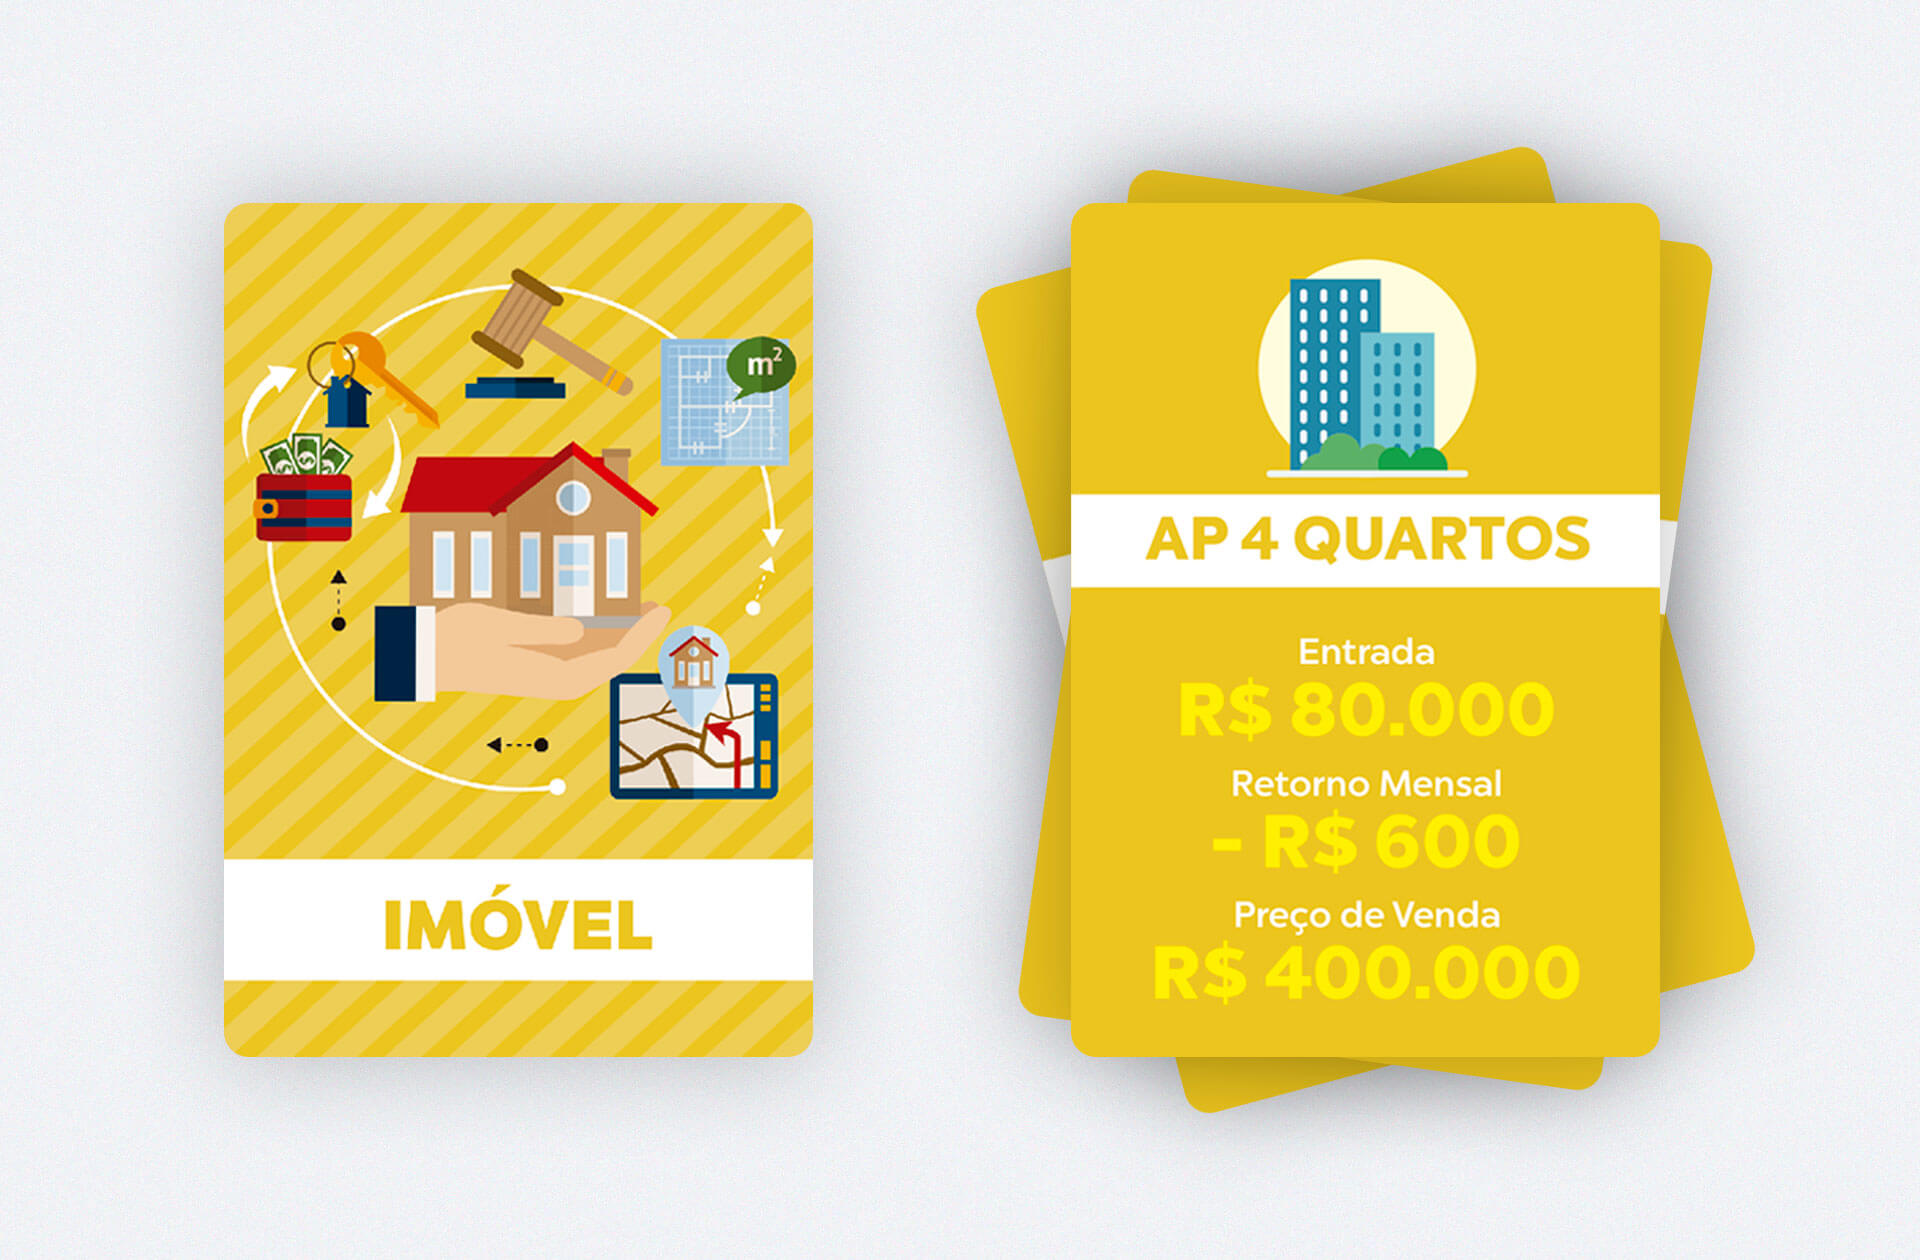
\includegraphics[width=0.8\textwidth]{figuras/fig12-carta-imovel.jpg}
\legend{\footnotesize Fonte: Frechiane, Manual do Jogo (\citeyear{frechiani2019b})}
\label{fig: fig12-carta-imovel}
\end{minipage}
\end{figure}

A carta cinza (figura \ref{fig: fig13-carta-oferta}), representada pelo pin de mesma cor, simboliza ofertas de compras para as cartas de imóvel e negócio obtido pelos personagens. Para conseguir uma oferta o jogador precisa movimentar seu personagem até o cenário mercado (figura \ref{fig: figura08-tabuleiro}) e retirar uma carta, a oferta só poderá ser concretizada caso o jogador possua a carta de imóvel ou de negócio com o mesmo tipo e nome que consta na carta de oferta. Caso a oferta seja relativo à um negócio o preço de venda é o que está anotado na carta de oferta, mas se a oferta é referente à um imóvel o jogador poderá escolher o preço de venda da carta de oferta ou da carta do seu imóvel.

\graphicspath{{figuras/}}
\begin{figure}[!ht]
\centering
\begin{minipage}{0.8\textwidth}
\caption{Renda Passiva (Carta Oferta)}
\centering
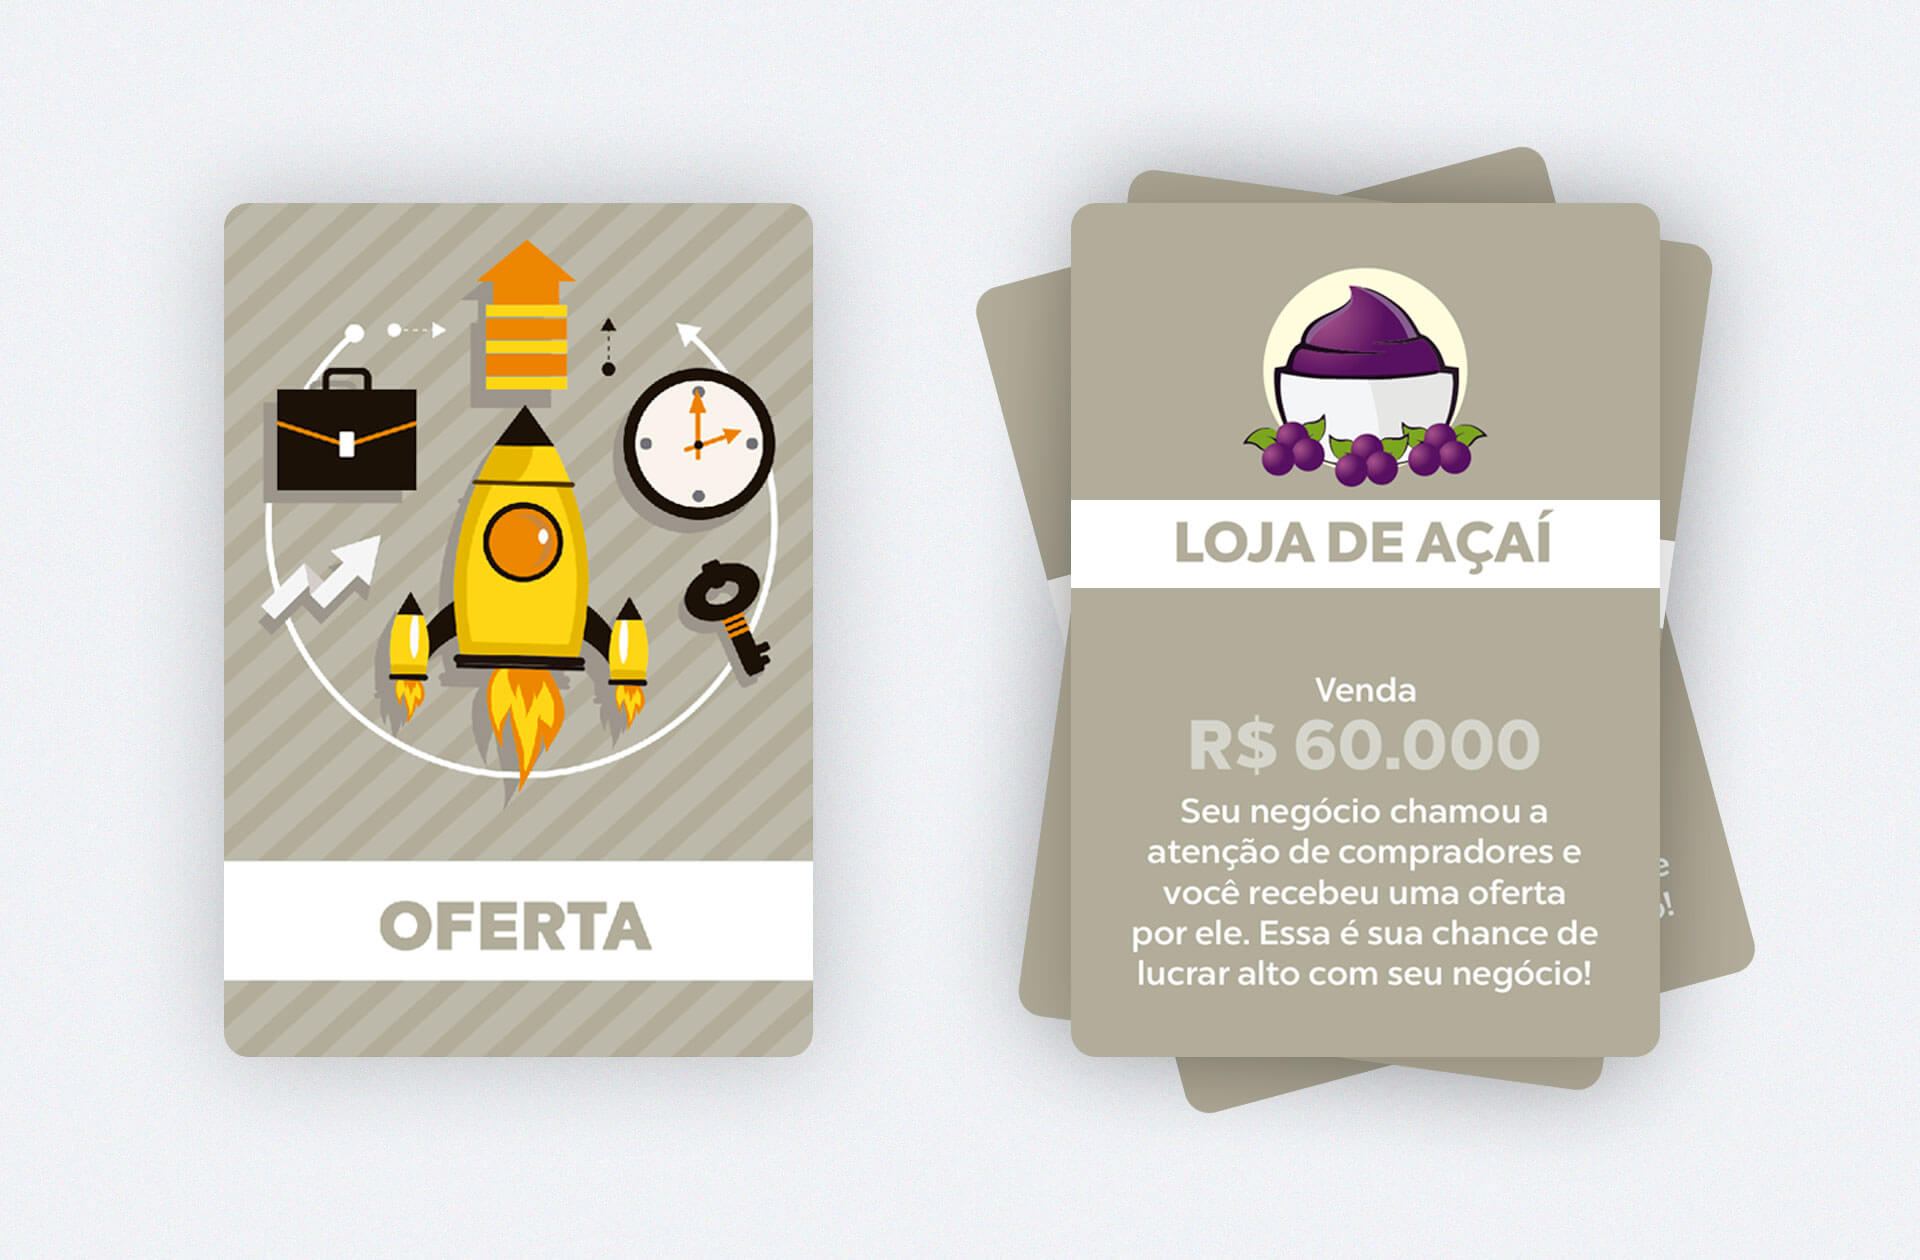
\includegraphics[width=0.8\textwidth]{figuras/fig13-carta-oferta.jpg}
\legend{\footnotesize Fonte: Frechiane, Manual do Jogo (\citeyear{frechiani2019b})}
\label{fig: fig13-carta-oferta}
\end{minipage}
\end{figure}

Para retirar a carta de renda fixa o jogador precisa conduzir seu personagem até o cenário banco. Esta carta oferece ao personagem uma aplicação de renda fixa dos tipos CDB, Tesouro Direto e LCI com seus respectivos valores mínimos (preços ou entrada), rentabilidade (retorno mensal) e liquidez. Esta carta apresenta exemplo dos principais tipos de investimento em renda fixa atuais do mercado financeiro nacional.

A figura \ref{fig: fig14-cenários} exibe um resumo dos cenários com seus respectivos \textit{pins} e cartas que poderão ser retiradas. Cada cenário possui sua casa de entrada e suas casas de saídas indicadas por setas laranjas no tabuleiro (figura \ref{fig: figura08-tabuleiro}). Cabe ao jogador decidir, de acordo com seus planos e objetivos de jogo, efetivar ou não as transações oferecidas pelas cartas, podendo recorrer ao financiamento bancário para efetuar a transação, exceto da carta surpresa que é de execução obrigatória.

\graphicspath{{figuras/}}
\begin{figure}[!ht]
\centering
\begin{minipage}{0.8\textwidth}
\caption{Renda Passiva (Cenários do Jogo)}
\centering
\includegraphics[width=0.8\textwidth]{figuras/fig14-cenários.PNG}
\legend{\footnotesize Fonte: Frechiane, Manual do Jogo (\citeyear{frechiani2019b})}
\label{fig: fig14-cenários}
\end{minipage}
\end{figure}

A carta variação (figura \ref{fig: fig15-carta-variação}) pode ser retirada em qualquer posição do tabuleiro na vez de cada jogador, ela modifica os valores das ações durante uma rodada ou até outro jogador virar uma nova carta. O preço inicial de cada ação é R\$25, contudo, as ações sofrerão ajustes de preço de acordo com os valores descritos na carta de variação escolhida pelo jogador, podendo aumentar ou diminuir o valor de cada ação, utilizando como exemplo a carta de variação da figura \ref{fig: fig15-carta-variação}, a ação da cor azul passará a valer R\$ 40 (R\$ 25 do valor inicial, mais R\$ 15 de variação) e a verde R\$ 14. A dinâmica desta carta, em conjunto com a carta surpresa de dividendos, fornece uma visão inicial aos alunos do funcionamento e estratégias de aplicações em renda variável.

\graphicspath{{figuras/}}
\begin{figure}[!ht]
\centering
\begin{minipage}{0.8\textwidth}
\caption{Renda Passiva (Carta Variação)}
\centering
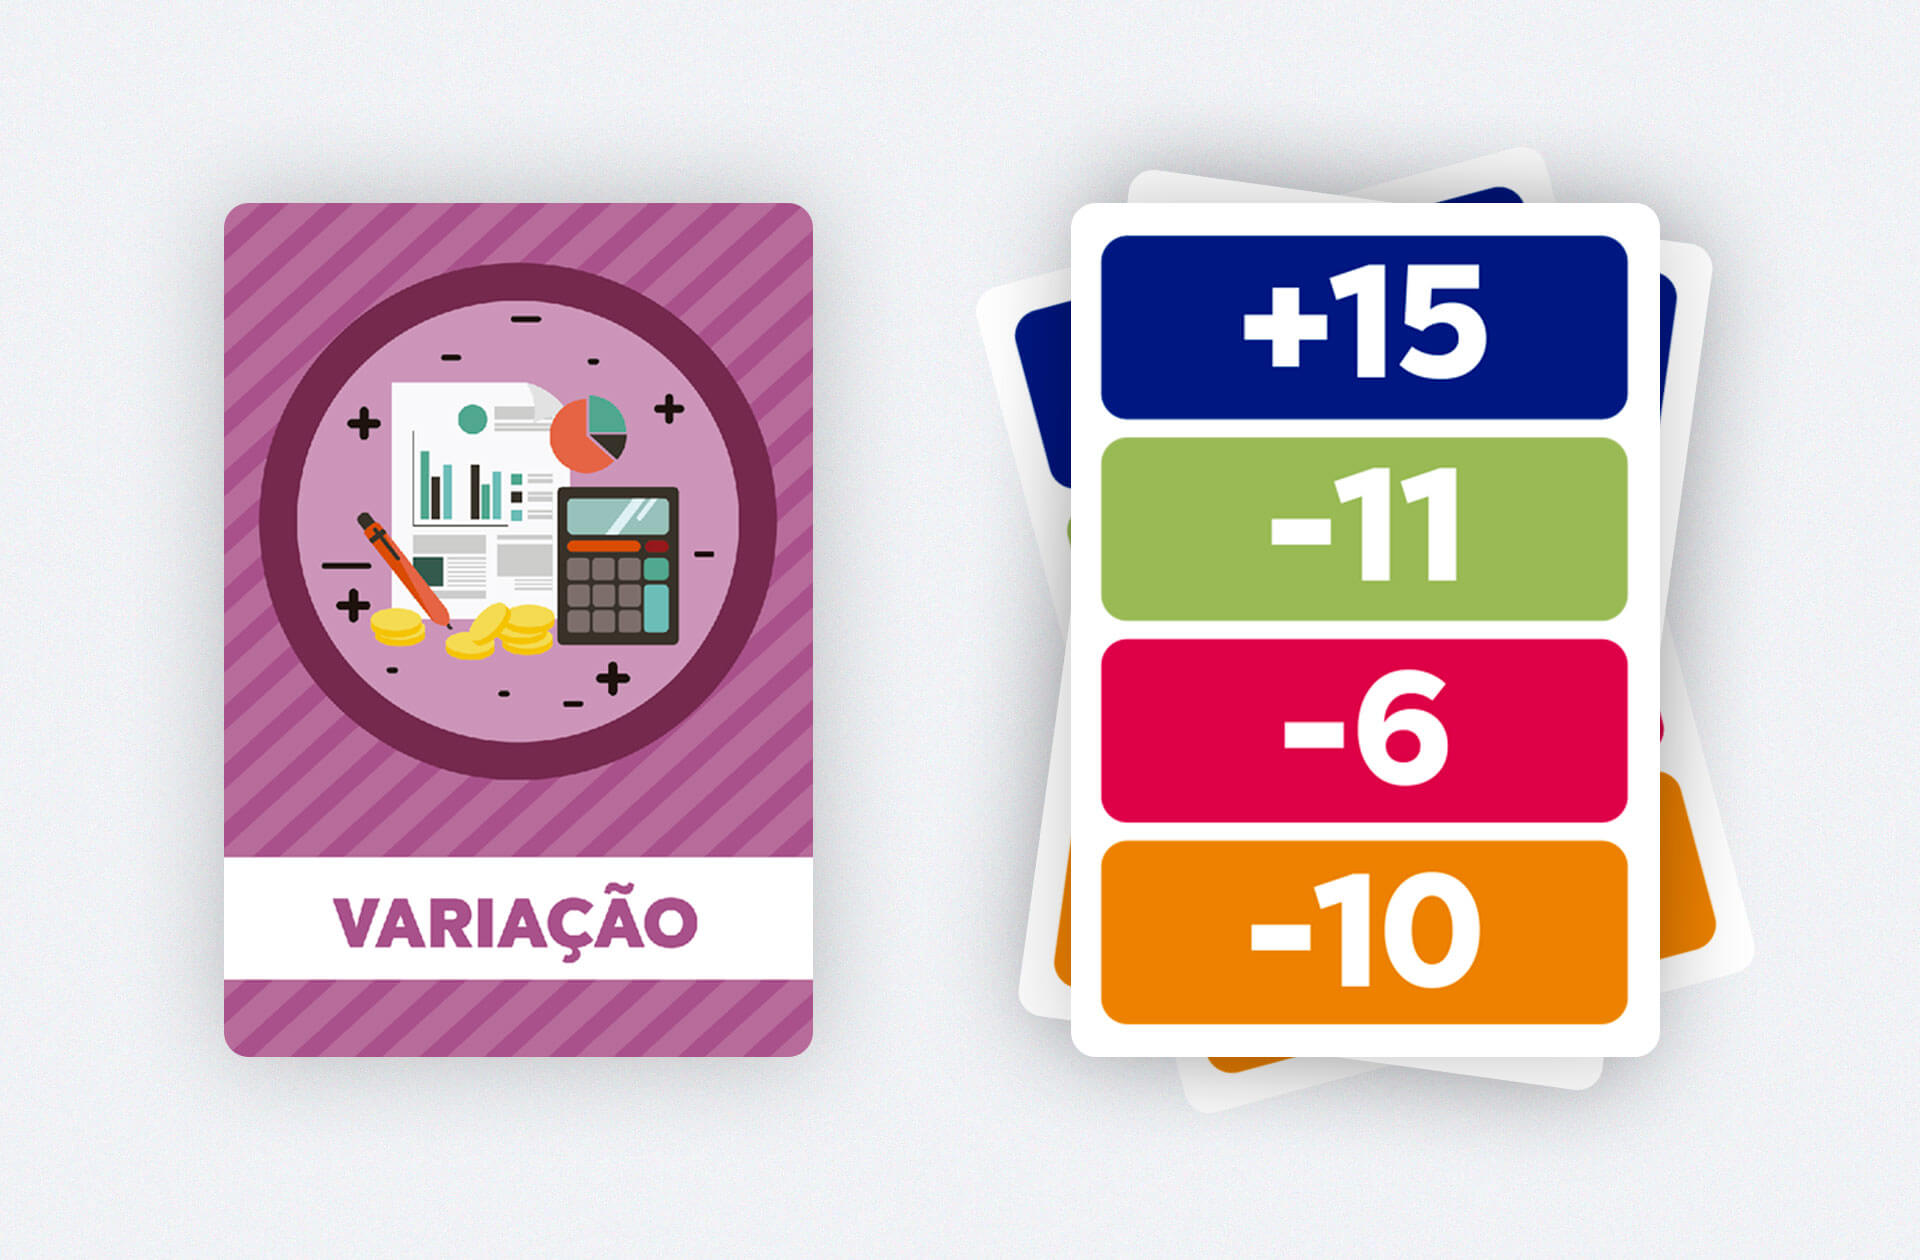
\includegraphics[width=0.8\textwidth]{figuras/fig15-carta-variação.jpg}
\legend{\footnotesize Fonte: Frechiane, Manual do Jogo (\citeyear{frechiani2019b})}
\label{fig: fig15-carta-variação}
\end{minipage}
\end{figure}

Diferente da maior parte dos jogos sobre finanças que possui um caminho único e cíclico, no Renda Passiva o jogador pode decidir por qual caminho seguir no tabuleiro de acordo com o planejamento que possui e assim determinar uma estratégia de jogo, sendo capaz de decidir entre quitar as dívidas, investir em ações ou renda fixa, comprar imóveis ou negócios, considerando o risco, a liquidez e a rentabilidade de cada item. Para isso basta apenas movimentar-se para os respectivos cenários (quadrados maiores com placas de mercado, cidade, aeroporto, loja, parque e banco) e retirar uma carta, exceto as cartas ações que podem ser solicitadas em qualquer posição. Dessa forma, o jogo proporciona ao jogador tentar construir diversas soluções possíveis para cada problema proposto pelo de forma segura. A cada nova solução concebida, aumenta a compreensão dos alunos a respeito do processo de solução dos problemas financeiros propostos pelo jogo.

O jogador que conseguir cumprir os 3 objetivos do jogo: quitar todas as dívidas, ter uma renda passiva igual ou maior ao seu total de gastos, chegar ao cenário conquista da liberdade financeira do tabuleiro (figura \ref{fig: figura08-tabuleiro}) vence o jogo. As regras podem ser modificadas para facilitar a compreensão, a aprendizagem e diminuir o tempo de jogo para encaixá-lo nas aulas.

No curso “Educação Financeira através de Jogos” cada ficha financeira do jogo Renda Passiva é administrada por uma dupla de alunos ou individualmente, a critério de cada aluno com auxílio do professor, as decisões financeiras do personagem durante o jogo devem ser discutidas e tomadas sob o consenso dos dois discentes no caso de duplas. Desse modo, por meio dos desafios financeiros propostos no jogo cada aluno pode perceber os erros e acertos em suas tomadas de decisões financeiras, permitindo aos alunos a possibilidade de testar os conhecimentos teóricos adquiridos em uma simulação simples, podendo ver as consequências de suas ações de forma rápida em um ambiente seguro.

\subsection{Avaliação da Utilização dos Jogos na Aprendizagem}
A utilização dos jogos Orçamento Consciente e Renda Passiva na aprendizagem dos alunos durante as aulas do curso foi avaliada utilizando o método MEEGA+, esse instrumento foi utilizado com o propósito de averiguar se os jogos favoreceram a aprendizagem da educação financeira, a partir da percepção e experiência dos discentes. Nesse sentido, aplicou-se os questionários do respectivo método, no formato impresso, logo após a interação dos alunos com jogos, a fim de recolher os dados necessários para produzir os resultados da avaliação.

O método MEEGA+ possui um questionário para avaliar a experiência subjetiva do jogador, permitindo a coleta de dados sobre diversos aspectos como o foco da atenção, diversão, desafio, interações sociais, relevância, satisfação, usabilidade e percepção de aprendizagem \cite{petri2017}, também apresenta uma seção para os jogadores relatarem os pontos fortes, fracos e comentários adicionais. Este método busca agir de forma rápida e não intrusiva para maior efetividade em avaliar a qualidade e a utilização dos jogos para aprendizagem.

A percepção de aprendizagem, os relatos dos discentes sobre os pontos fortes, fracos e comentários adicionais são utilizados como critérios principais para avaliar se os jogos Orçamento Consciente e Renda Passiva contribuíram para a aprendizagem na percepção dos alunos, por isso os outros aspectos relacionados ao método foram considerados menos relevante para este estudo. Espera-se que os resultados dos dados obtidos com os questionários do MEEGA+ e analisados por uma abordagem qualitativa possam confirmar que os jogos utilizados favoreceram a aprendizagem dos discentes, atendendo aos objetivos da presente pesquisa.

\section{AS AVALIAÇÕES}
A avaliação da efetividade do curso “Educação Financeira através de Jogos” ocorreu em três fases, na primeira fase os alunos responderam aos questionários impressos de aprendizagem, de avaliação da aprendizagem (Apêndice \ref{apend-a}) e de avaliação do curso (Apêndice \ref{apend-b}) após a última aula do curso. Na segunda fase, após um ano do início do curso, aplicou-se digitalmente o questionário de aplicação do conhecimento (Apêndice \ref{apend-c}). Na derradeira fase se realizou a análise dos dados levantados com os questionários propostos, produzindo assim os resultados da pesquisa.

O questionário de avaliação da aprendizagem (Apêndice \ref{apend-a}) foi elaborado para aferir o nível de retenção dos alunos em relação ao conteúdo apresentado durante o curso. O questionário de avaliação do curso (Apêndice \ref{apend-b}) para verificar o conhecimento prévio, a motivação para participar do curso, o interesse em buscar novos conhecimentos, a disseminação do conhecimento adquirido e a consciência da importância do tema estudado pelos estudantes. E o de aplicação do conhecimento (Apêndice \ref{apend-c}) para averiguar se os alunos e/ou seus familiares estão utilizando os conceitos financeiros adquiridos no curso e em quais níveis dos estágios do letramento financeiro, bem como averiguar se o conteúdo aprendido no curso está auxiliando a superar os problemas financeiros causados pela pandemia do COVID-19 e de qual forma.

Os dados da presente pesquisa, recolhidos por intermédio dos questionários, foram analisados utilizando a abordagem qualitativa, com o objetivo de verificar a efetividade do curso “Educação Financeira através de Jogos”, bem como se o jogos e a metodologia do curso contribuíram no processo de aprendizagem, aferir o nível de retenção dos temas principais apresentados, o conhecimento prévio, a motivação para participar do curso, o interesse em buscar novos conhecimentos, a disseminação do conhecimento adquirido e a relevância do tema na perspectiva dos alunos, e também verificar se os discentes estão aplicando o conhecimento adquiridos em suas vidas e em quais níveis dos estágios do desenvolvimento cognitivo do letramento financeiro.

Os dados coletados no retorno dos questionários respondido pelos alunos, possibilitarão aos pesquisadores categorizar e analisar as respostas no intuito de verificar quais objetivos propostos foram atingidos e a averiguar a confirmação ou não da hipótese. Ao refletir sobre os dados coletados, espera-se chegar à conclusão sobre a potencialidade que o curso oferece, bem como se a metodologia utilizada e os jogos possibilitaram e facilitaram aquisição do conhecimento relativo aos conteúdos abordados. Nesse sentido, houve a necessidade de estabelecer critérios para avaliar os dados coletados e realizar a análise dos resultados.

\subsection{Critérios para Análise dos Dados e Resultados}
As respostas dos alunos no questionário de aprendizagem foram agregadas por questões e por alunos para verificar as dificuldades e o desempenho de cada estudante nas questões.

O capítulo XIX da organização didática do IFSUL trata sobre a avaliação das aprendizagens e estabelece que o aluno precisa obter uma nota igual ou superior a 6,0 para ser aprovado em um componente curricular \cite{ifsul2012}. Esse mesmo critério foi utilizado para analisar os resultados do questionário de aprendizagem, assim, para o aluno obter um bom resultado na aprendizagem, ele necessita acertar no mínimo 60\% das questões e para afirmar que o tema de uma questão foi compreendido pelos alunos, ela precisa ter sido respondida corretamente por no mínimo 60\% dos discentes. Do mesmo modo, para afirmar que a aprendizagem foi efetiva e que os alunos obtiveram um bom nível de retenção a média de acerto dos estudantes e a média de acerto das questões deverão ser superior ou igual a 60\%.

Conforme apresentado em capítulos anteriores, o objetivo geral da presente proposta é avaliar a efetividade do curso “Educação Financeira através de Jogos”, nessa perspectiva para definir se o curso foi bem avaliado e produziu os resultados esperados foram definidos critérios que estão descritos no quadro \ref{quad: quadro-05-criterios-avaliacao-curso}, em conjunto com os respectivos instrumentos avaliativos e questões utilizadas na obtenção dos dados.

\graphicspath{{quadros/}} 
\begin{quadro}[!ht]
\centering
\begin{minipage}{0.8\textwidth}
\caption{Critérios de Avaliação do Curso}
\centering
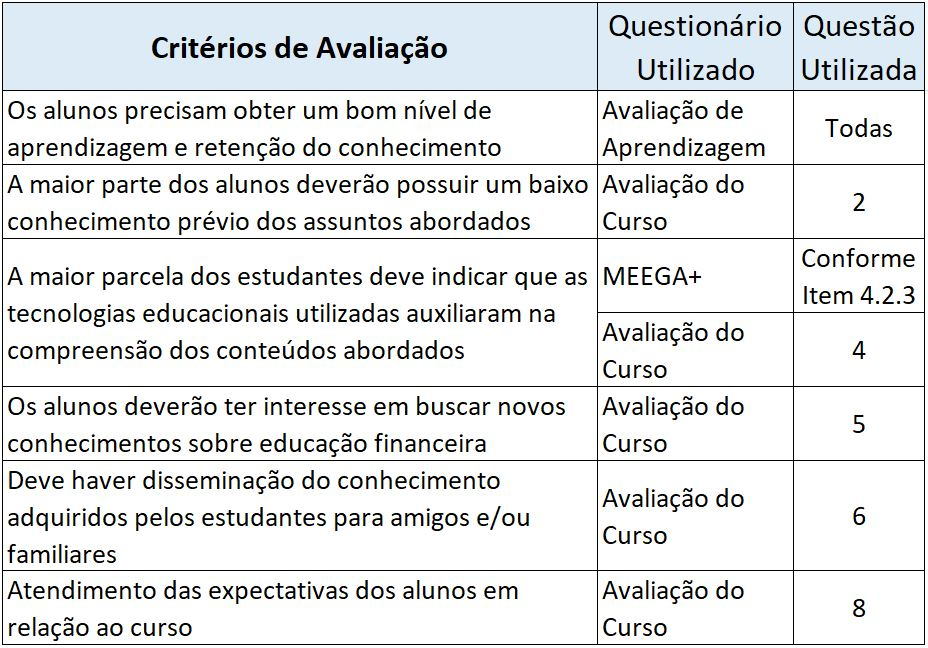
\includegraphics[width=1.0\textwidth]{quadro-05-criterios-avaliacao-curso}
\legend{\footnotesize Fonte: O Autor, 2019}
\label{quad: quadro-05-criterios-avaliacao-curso}
\end{minipage}
\end{quadro}
\newpage
Por fim, os dados retornados do questionário de aplicação do conhecimento são utilizados para verificar se o conhecimento adquirido pelos alunos auxiliou a enfrentar as dificuldades financeiras causadas pela pandemia do COVID-19, proporcionou mudanças na vida dos estudantes e de sua família, assim como, indicar o estágio de desenvolvimento cognitivo do letramento financeiro de cada aluno, considerou-se os hábitos e comportamentos inerentes a cada estágio, assim como os aspectos socioeconômicos do estudante, como critério para perceber o estágio de desenvolvimento cada estudante após um ano de início do curso..

\chapter{PRODUTO: CURSO EDUCAÇÃO FINANCEIRA ATRAVÉS DE JOGOS}
Conforme citado em capítulos anteriores, o produto desta pesquisa é o curso de “Educação Financeira através de Jogos” para ensino médio integrado, voltado inicialmente para os institutos federais e outras autarquias da RFEPCT. Com base no referencial teórico e nos trabalhos diretamente relacionados ao tema pesquisado, foi possível estabelecer 5 unidades temáticas que são abordadas no decorrer do curso: matemática financeira, finanças comportamentais, consumo consciente, instituições financeiras e serviços, investimentos e previdência.

O conteúdo tratado no curso é ministrado em 8 encontros com 2 aulas de 45 minutos cada, o quadro \ref{quad: quadro-06-unidade-tematicas-curso} elenca o conjunto das unidades temáticas do curso os respectivos conteúdos programáticos. O objetivo instrucional, conhecimento prévio, recursos utilizados, tema e desenvolvimento de cada encontro estão descritos no decorrer deste capítulo.

\graphicspath{{quadros/}} 
\begin{quadro}[!ht]
\centering
\begin{minipage}{0.9\textwidth}
\caption{Unidade Temáticas e Conteúdos Programáticos do Curso}
\centering
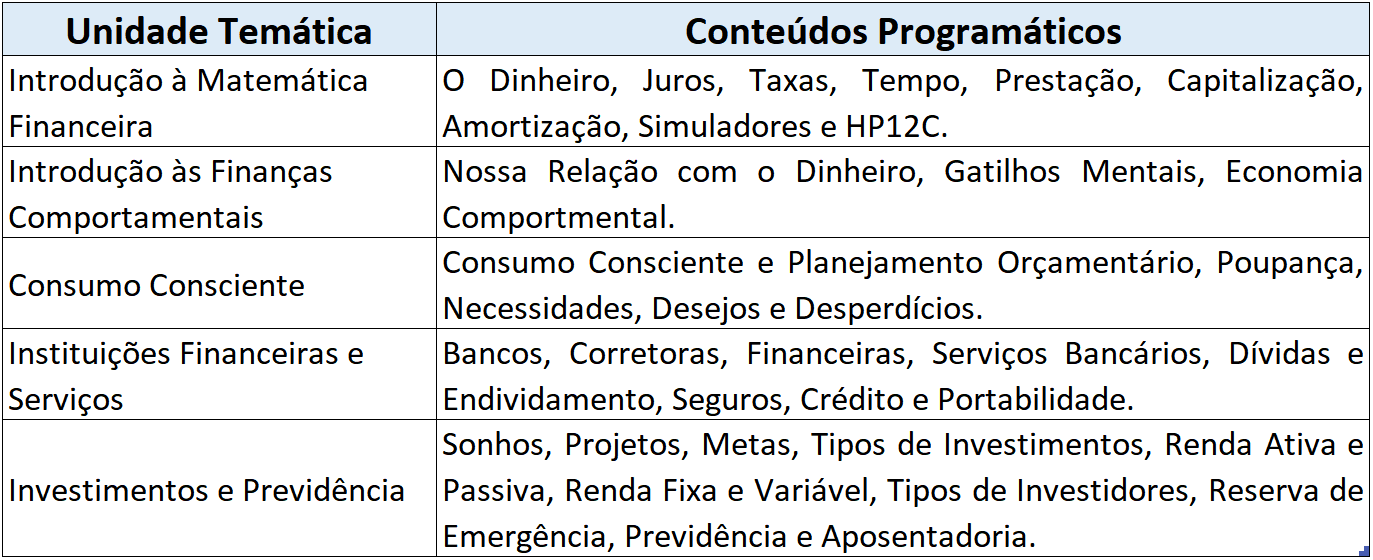
\includegraphics[width=1.0\textwidth]{quadro-06-unidade-tematicas-curso}
\legend{\footnotesize Fonte: O autor, 2019}
\label{quad: quadro-06-unidade-tematicas-curso}
\end{minipage}
\end{quadro}

\section{1º ENCONTRO - MATEMÁTICA FINANCEIRA}
Quando possível, o primeiro encontro deve ser ministrado por um docente especialista em matemática financeira e educação, pois este, teoricamente, detém um domínio mais amplo sobre o conteúdo abordado na aula. Para desenvolver o tema do primeiro encontro os alunos deverão possuir conhecimentos básicos sobre o Sistema Monetário Brasileiro principalmente sobre formas de trocar recursos financeiros por serviços ou produtos e reconhecer os signos monetários, aprendizado este adquirido nos anos iniciais do ensino fundamental e na vivência do aluno. O quadro \ref{quad: quadro-07-aula 1} apresenta o plano de aula do 1º encontro no qual é abordado especificamente a unidade temática introdução à matemática financeira.

\graphicspath{{quadros/}}
\begin{quadro}[!ht]
\centering
\begin{minipage}{0.8\textwidth}
\caption{Plano de Aula 1º Encontro}
\centering
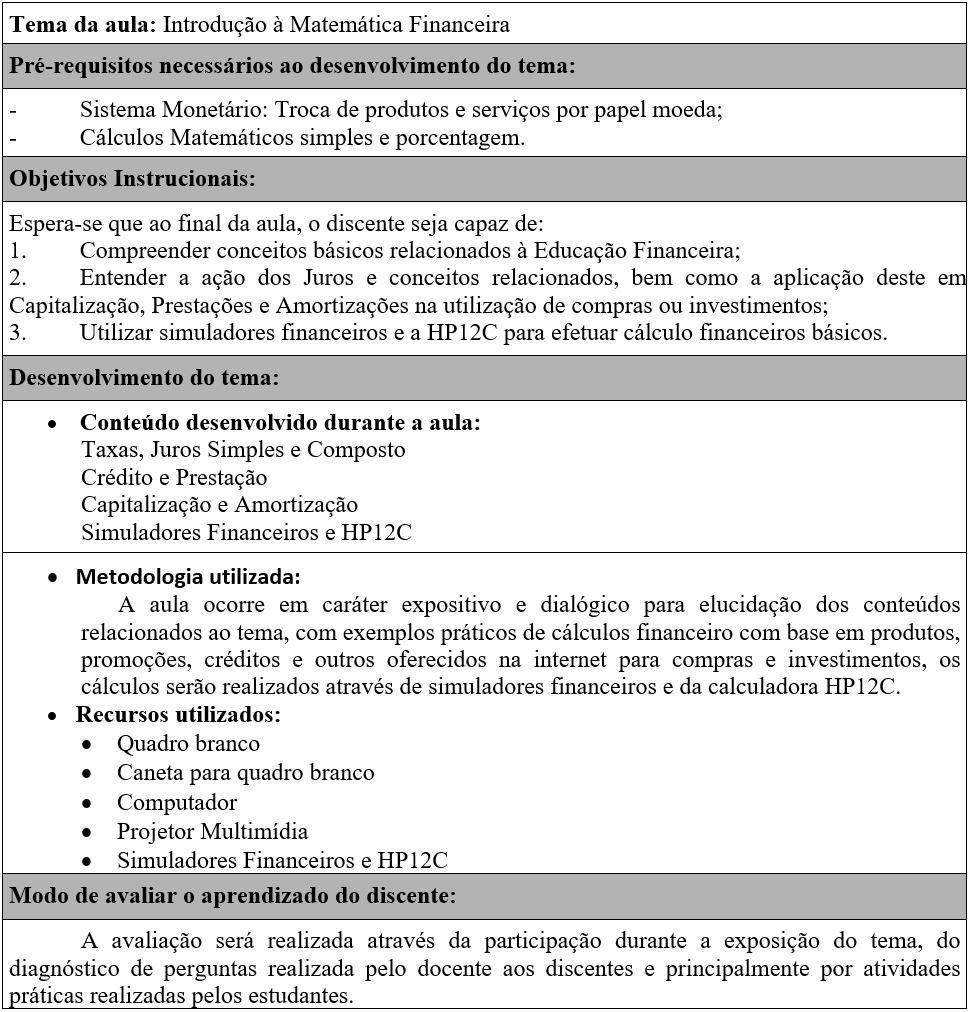
\includegraphics[width=0.9\textwidth]{quadro-07-aula 1.png}
\legend{\footnotesize Fonte: O autor, 2019}
\label{quad: quadro-07-aula 1}
\end{minipage}
\end{quadro}

Este encontro é dividido em duas etapas, na primeira são expostos oralmente para os aluno conceitos iniciais relacionados aos temas propostos que estão descritos no quadro \ref{quad: quadro-07-aula 1}, com auxílio de recursos tecnológicos multimídias como apresentação de slides elaboradas pelos discentes e vídeos como o do canal Nerdologia do \textit{Youtube} (https://www.youtube.com/watch?v=5vpixQc3b2M) que elucida o conceito de dinheiro e sua invenção para ser utilizado como moeda de troca, tais instrumentos são utilizados para facilitar a introdução de temas desconhecidos pelos discente, outros recursos podem ser adicionados para auxiliar o processo. Em seguida o professor realiza a comparação na aquisição de um produto no formato a vista e a prazo como exemplo, calculando o juros, a amortização e as prestações, exemplificando para os alunos como realizar os cálculos necessários para comparar os modos de pagamentos para aquisição de serviços e produtos.

Na segunda etapa do encontro é realizado uma atividade prática na qual cada aluno escolhe um produto ou serviço que deseja obter, tais como a compra de um celular, vídeo game, retirar carteira nacional de habilitação, entre outros, após a escolha do serviço ou produto desejado os alunos devem pesquisar na internet as formas de pagamento para adquiri-los, calculando os juros embutidos, as parcelas, a amortização, também devem simular uma opção de compra na qual poupam dinheiro e aplicam a uma taxa mínima do mercado, estipulado pelo professor, efetuando a compra à vista posteriormente com o montante poupado. Ao final da atividade os cálculos da compra a prazo e à vista são comparados para que os alunos aprendam a verificar diferenças e vantagens de cada opção de compra. Para realizar os cálculos financeiros durante a aula, são utilizados exemplos de produtos que façam parte do vida dos discentes para estimular o processo de aprendizagem, também são utilizados simuladores financeiros ou da calculadora HP12C e de juros compostos ou de correções de valores como a calculadora do cidadão do BACEN (https://www3.bcb.gov.br/CALCIDADAO/jsp/index.jsp). Durante a atividade prática é importante que o professor estimule o debate entre os alunos sobre as vantagens e desvantagens dos modos de pagamentos escolhidos a fim de promover a reflexão acerca do assunto abordado.

\section{2º ENCONTRO - FINANÇAS COMPORTAMENTAIS}
No segundo encontro é trabalhado com os discentes a unidade temática referente à introdução às finanças comportamentais. Os conteúdos, os objetivos e a temática da aula estão descritos no plano de aula do 2º encontro, apresentado no quadro \ref{quad: quadro-08-aula 2}.

\graphicspath{{quadros/}} 
\begin{quadro}[!ht]
\centering
\begin{minipage}{0.8\textwidth}
\caption{Plano de Aula 2º Encontro}
\centering
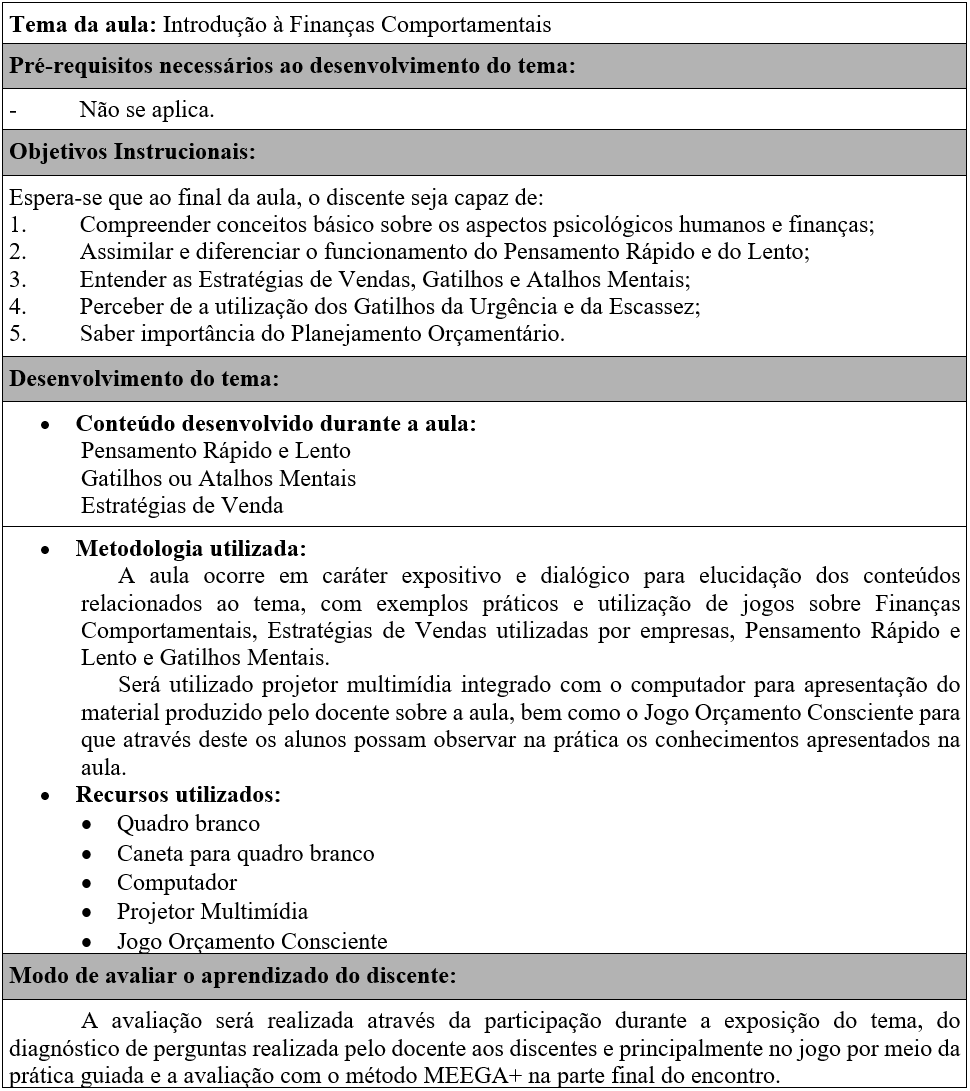
\includegraphics[width=0.9\textwidth]{quadro-08-aula 2}
\legend{\footnotesize Fonte: O autor, 2019}
\label{quad: quadro-08-aula 2}
\end{minipage}
\end{quadro}

No início desse encontro o professor deve oralmente introduzir conceitos sobre heurísticas e vieses do comportamento humano relacionados às finanças, através de exemplos e debates com os alunos, também deve apresentar concepções acerca das formas do pensamento humano para tomada de decisões proposta por Kahneman, bem como as estratégias de venda apontadas por Cialdini. Após a explanação inicial, os estudantes interagem com o jogo Orçamento Consciente por intermédio do computador, cada discente interage individualmente com o jogo ou em dupla (dependendo da proposta da aula), desta forma o aluno pode observar, praticar, associar e obter melhor compreensão sobre os temas abordados em aula. Após utilizar o jogo é importante conversar com os alunos sobre os aprendizados da aula observados no jogo, a percepção dos alunos em relação aos gatilhos mentais e ao pensamento rápido e lento. Caso julgue necessário o professor pode utilizar o jogo através de \textit{smartphones} ou \textit{tablets}.

Estruturou-se o segundo encontro com o intuito de auxiliar o processo de ensino-aprendizagem de finanças comportamentais, bem como no desenvolvimento cognitivo do letramento financeiro do estudante, para que este inicie a transição do estágio Consumidor Sensorial (consumo baseado em sensações) para o Consumidor Pré-Poupador (consumo consciente dos recursos financeiros), assim como assimilar a importância do planejamento orçamentário.

\section{3º ENCONTRO - CONSUMO CONSCIENTE}
Após os discentes aprenderem sobre conceitos básicos da matemática financeira, finanças comportamentais e entender a importância de planejar seus gastos, a unidade temática do terceiro encontro apresenta o consumo consciente relacionado às finanças, no intuito de demonstrar como executar o planejamento orçamentário familiar e/ou pessoal. Os conteúdos relacionados à unidade temática do 3º encontro estão elencados no quadro \ref{quad: quadro-09-aula 3}, por meio do plano de aula.

\graphicspath{{quadros/}} 
\begin{quadro}[!ht]
\centering
\begin{minipage}{0.8\textwidth}
\caption{Plano de Aula 3º Encontro}
\centering
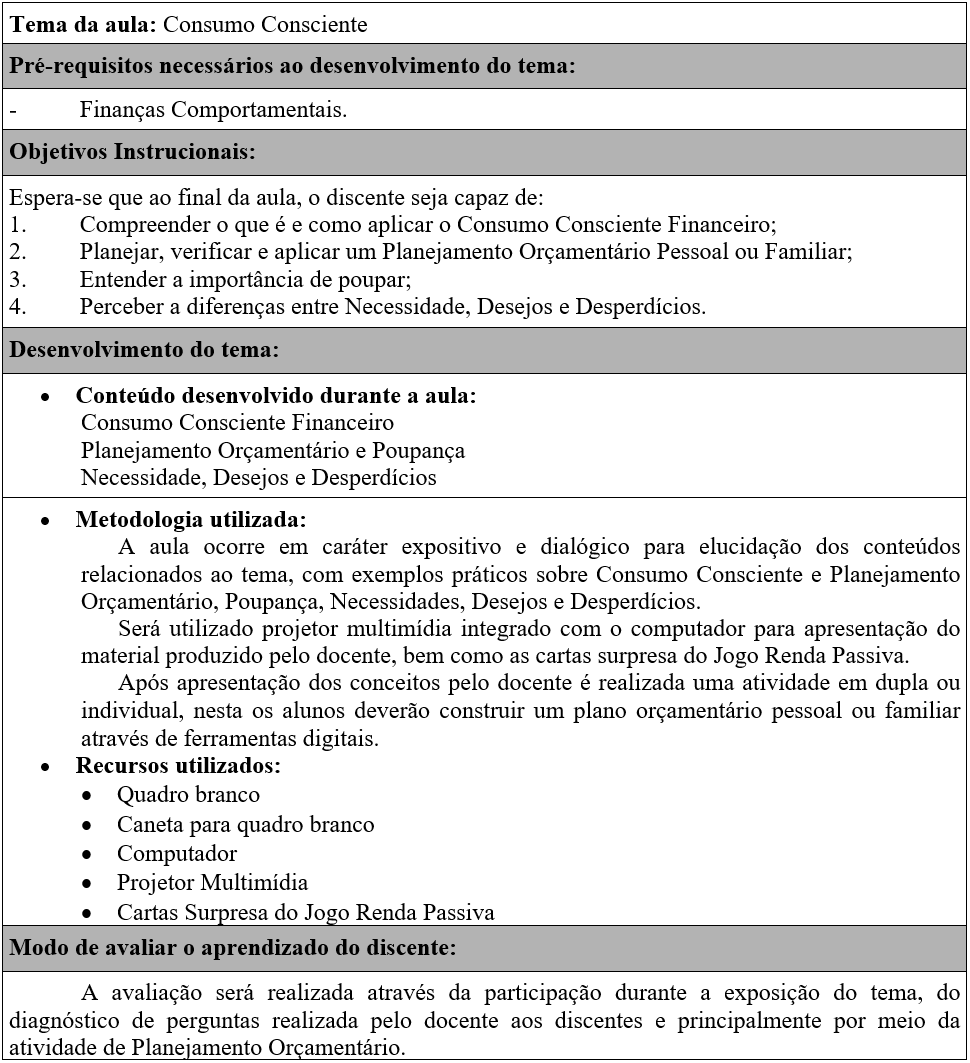
\includegraphics[width=0.9\textwidth]{quadro-09-aula 3}
\legend{\footnotesize Fonte: O autor, 2019}
\label{quad: quadro-09-aula 3}
\end{minipage}
\end{quadro}
\newpage
Nesse encontro o professor deve apresentar aos alunos conceitos sobre o consumo consciente, trabalhar os conteúdos relacionados ao planejamento orçamentário, ao tipos e partes do orçamento e à diferença entre necessidades, desejos e desperdícios, bem como demonstrar para os alunos a importância de não utilizar toda a receita recebida no mês. Esse conteúdo do curso pode ser apresentado oralmente aos alunos com auxílio de uma apresentação multimídia utilizando \textit{slides}. Devem ser apresentados também aos estudantes aplicativos e ferramentas financeiras que auxiliam no planejamento orçamentário como o GuiaBolso (https://www.guiabolso.com.br/), Mobilis (https://www.mobills.com.br/) ou as planilhas de orçamento doméstico, como exemplo a do Instituto Brasileiro de Defesa do Consumidor-IDEC (https://idec.org.br/ferramenta/planilha-de-orcamento-domestico).

Após a exposição teórica do conteúdo aos discente deve ser realizada uma atividade de planejamento orçamentário, individual (pessoal) ou em dupla (familiar), essa escolha pode ser a critério do docente, na atividade os estudantes devem definir uma profissão que almejam trabalhar, buscar o salário médio respectivo e defini-lo como receita mensal, o orçamento também deve conter despesas com habitação (aluguel e condomínio), saúde, transporte, educação, contas residenciais e alimentação. Para o gasto com habitação os alunos deverão procurar o aluguel de uma residência na qual deseja morar e que encaixe em seus respectivos orçamentos financeiros, para outras categorias de despesas o professor definirá um valor fixo por pessoa da família, os discentes devem poupar o máximo possível de suas receitas no orçamento.

Com o orçamento mensal dos alunos finalizado começa a segunda parte da atividade que tem o intuito de demonstrar aos alunos que imprevistos acontece, por isso a importância de realizar uma reserva financeira. Os estudantes devem retirar uma carta surpresa do jogo Renda Passiva que influenciará diretamente no orçamento financeiro realizado, tendo que alterá-lo para se adequar ao imprevisto trazido pela carta. As cartas surpresa do jogo Renda Passiva contêm oportunidades (restituição de imposto, bônus da empresa, promoção no trabalho, décimo terceiro etc.) e riscos como multas de trânsito, demissão, imposto, entre outros, como exemplo a carta que representa a chegada de um filho que aumenta a despesa em 10\% do salário (figura \ref{fig: fig16-carta-bebe}).

\graphicspath{{figuras/}} 
\begin{figure}[!ht]
\centering
\begin{minipage}{1.\textwidth}
\caption{Renda Passiva (Carta Surpresa Bebê a Caminho)}
\centering
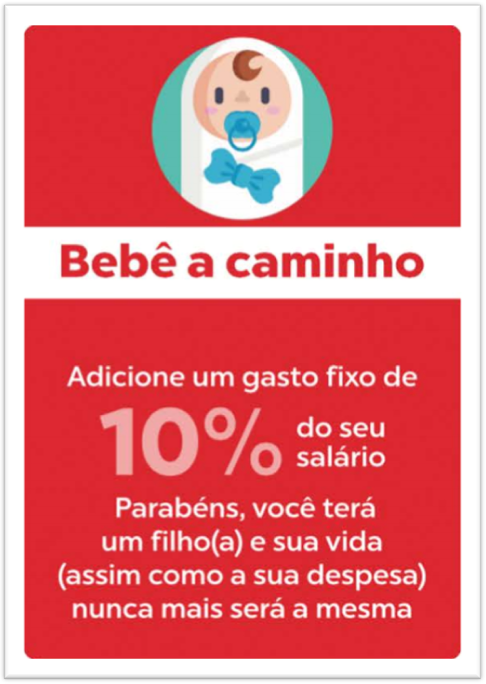
\includegraphics[width=0.3\textwidth]{fig16-carta-bebe}
\legend{\footnotesize Fonte: Frechiane (\citeyear{frechiani2019b})}
\label{fig: fig16-carta-bebe}
\end{minipage}
\end{figure}

O intuito desse encontro é proporcionar ao estudante conhecimento e indicar ferramentas que possam auxiliar no orçamento financeiro pessoal e familiar. Ao aplicar continuamente em sua vida e de sua família o conhecimento adquirido nessa aula, o aluno alcançará o segundo estágio do desenvolvimento cognitivo do letramento financeiro denominado Consumidor Pré-Poupador, consumindo de forma consciente com planos de aquisição de bens, produtos e serviços estabelecidos previamente, diminuindo o impacto das estratégias de vendas, gatilhos mentais em suas decisões de compras e consequentemente diminuindo também as compras por impulso.

\section{4º ENCONTRO - INSTITUIÇÕES FINANCEIRAS}
O objetivo do quarto encontro é explanar aos estudantes os tipos de instituições financeiras (bancos, corretoras de investimento, seguradoras e financeiras), suas diferenças e seus respectivos serviços (cesta de serviço, seguros, investimentos, crédito e portabilidade), bem como sobre dívidas e endividamento. Os conteúdos relacionados a unidade temática estão descritos no quadro \ref{quad: quadro-10-aula 4} que apresenta o plano de aula do 4º encontro.

\graphicspath{{quadros/}} 
\begin{quadro}[!ht]
\centering
\begin{minipage}{0.8\textwidth}
\caption{Plano de Aula 4º Encontro}
\centering
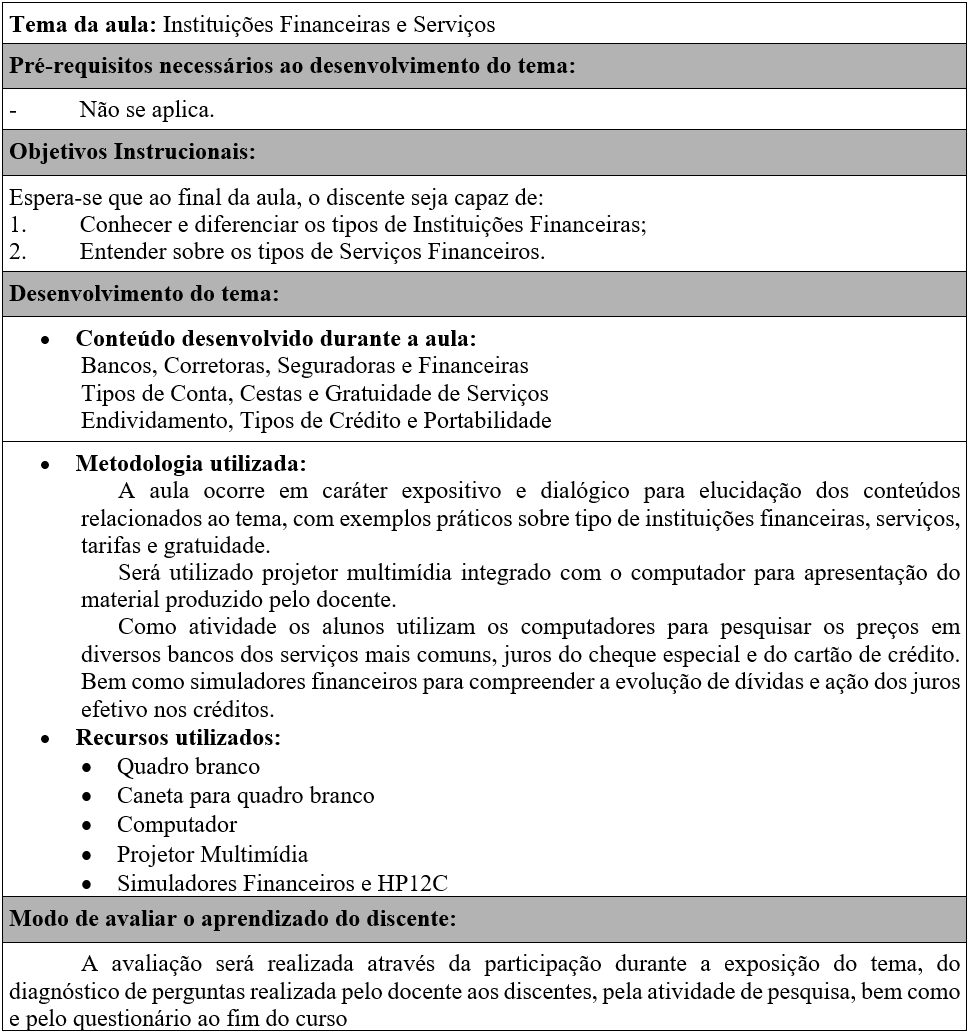
\includegraphics[width=0.9\textwidth]{quadro-10-aula 4}
\legend{\footnotesize Fonte: O autor, 2019}
\label{quad: quadro-10-aula 4}
\end{minipage}
\end{quadro}

Nesse encontro o professor deve trabalhar com os alunos principalmente os tipos de serviços que as instituições financeiras proporcionam aos clientes, tais como:

\begin{itemize}
    \item cestas de serviços bancários - utilizando sites dos principais bancos tradicionais e digitais para comparar os valores cobrados, assim como a resolução 3.919 do BACEN que normatiza a cobrança de tarifas e obriga todo banco oferecer uma conta corrente de serviços essenciais de forma gratuita;

    \item crédito - exemplificando e explicando os tipos de crédito mais utilizados e seus respectivos juros, entre eles, o cartão de crédito, cheque especial, créditos pessoal, consignado, estudantil, automotivo e portabilidade de crédito, simulando contratação de alguns desses serviços nos sites das financeiras;

    \item seguros - demonstrando a importância da contratação, as vantagens e desvantagens desse serviço e os tipos de seguros existentes, bem como os termos relacionados normalmente utilizados em contratos de aquisição de seguros;

    \item investimentos - explicar sucintamente o que é um investimento, a existência de outros tipos de aplicação além da poupança, comparar taxas de corretoras de investimento com bancos para realizar aplicações financeiras e abordar mais profundamente o que é a poupança e as regras atuais da caderneta de poupança.
\end{itemize}

Ao final desse encontro aplicando o conhecimento adquirido o aluno alcança o estágio Poupador Concreto do desenvolvimento cognitivo do letramento financeiro, pois compreende a importância e utiliza o planejamento orçamentário para alcançar um consumo financeiro mais consciente, busca sempre poupar recursos, conhece os tipos de serviços oferecidos pelas instituições financeiras, assim como investe o recurso poupado na caderneta de poupança, por falta de conhecimento em outros investimentos.

\section{5º ENCONTRO - INTRODUÇÃO AOS INVESTIMENTOS}
O objetivo do quinto encontro é demonstrar aos estudantes os aspectos relacionados à introdução de investimentos financeiros, bem como iniciar a transição do desenvolvimento cognitivo do letramento financeiro para o último estágio (Investidor Formal). Os conteúdos relacionados a unidade temática estão descritos no quadro \ref{quad: quadro-11-aula 5} que apresenta o plano de aula do 5º encontro.

\graphicspath{{quadros/}} 
\begin{quadro}[!ht]
\centering
\begin{minipage}{0.8\textwidth}
\caption{Plano de Aula 5º Encontro}
\centering
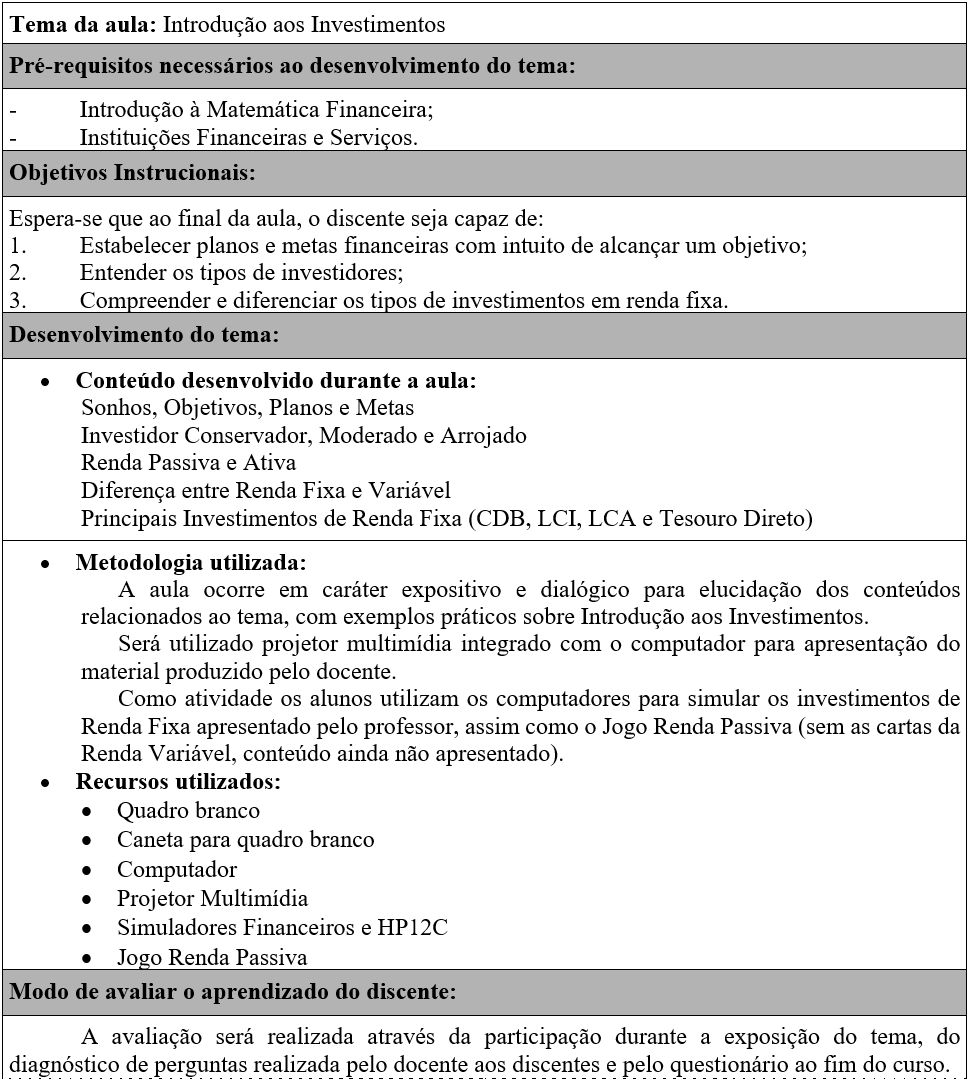
\includegraphics[width=0.9\textwidth]{quadro-11-aula 5}
\legend{\footnotesize Fonte: O autor, 2019}
\label{quad: quadro-11-aula 5}
\end{minipage}
\end{quadro}

\newpage
Nesse encontro o professor deve trabalhar com os alunos a diferença entre sonhos, objetivos, planos e metas, renda passiva e ativa, a distinção entre prazos (curto, médio e longo), a definição dos tipos de aplicações e investidores, apresentar aos alunos as principais aplicações de renda fixa que as instituições financeiras oferecem, os indexadores financeiros atrelados aos investimentos (CDI, IPCA e SELIC), assim como explanar sobre o Fundo Garantidor de Crédito (FGC), risco, liquidez e rentabilidade relacionado-os a cada ativo financeiro disponibilizado pelas principais corretoras de investimentos e bancos. Durante a aula o docente necessita utilizar simuladores financeiros para realizar simulações de investimentos em renda fixa, como os simuladores de juros composto e de investimento do \textit{blog} Me Poupe (https://mepoupenaweb.uol.com.br/simuladores-online-de-investimentos), e o simulador do tesouro direto (https://www.tesourodireto.com.br/simulador/). O professor também pode utilizar as cartas do Jogo Renda Passiva para introduzir o assunto, demonstrar o risco, a rentabilidade e a liquidez dos ativos financeiros, assim como explicar os tipos de investimentos em renda fixa e as diferenças entre este e a renda variável, esses recursos educacionais são utilizados com a finalidade de permitir a prática dos discentes e facilitar a compreensão.

Após a elucidação do conteúdo, o docente deve propor aos alunos uma atividade em que este deve refletir sobre um sonho de consumo, algo que deseja realizar ou comprar, e apresentar um projeto de aquisição do sonho com metas, prazo e valores bem definidos. Com o propósito de transformar o sonho em objetivo, o discente deve simular e planejar aportes financeiros mensais em uma aplicação financeira de renda fixa (tesouro direto ou CDB ou LCI/LCA) e escolher a mais adequada ao seu objetivo, considerando o prazo de aquisição do objetivo, o risco, a liquidez e a rentabilidade do investimento, optando pela aplicação mais rentável para alcançar o objetivo de compra, com o auxílio do professor e dos colegas. O aluno deve entregar a atividade contendo o objetivo e prazo para cumpri-lo, metas, aportes mensais e aplicação escolhida para alcançar o desejo de consumo escolhido.

\section{6º ENCONTRO - REVISÃO COM O JOGO RENDA PASSIVA}
O objetivo do sexto encontro é revisar junto aos discentes os conteúdos abordados no curso (finanças comportamentais, planejamento orçamentário, portabilidade de crédito e investimentos), bem como a acomodação dos conteúdos estudados através do jogo sério Renda Passiva. O plano de aula deste encontro está descrito no quadro \ref{quad: quadro-12-aula 6}.

\graphicspath{{quadros/}} 
\begin{quadro}[!ht]
\centering
\begin{minipage}{0.8\textwidth}
\caption{Plano de Aula 6º Encontro}
\centering
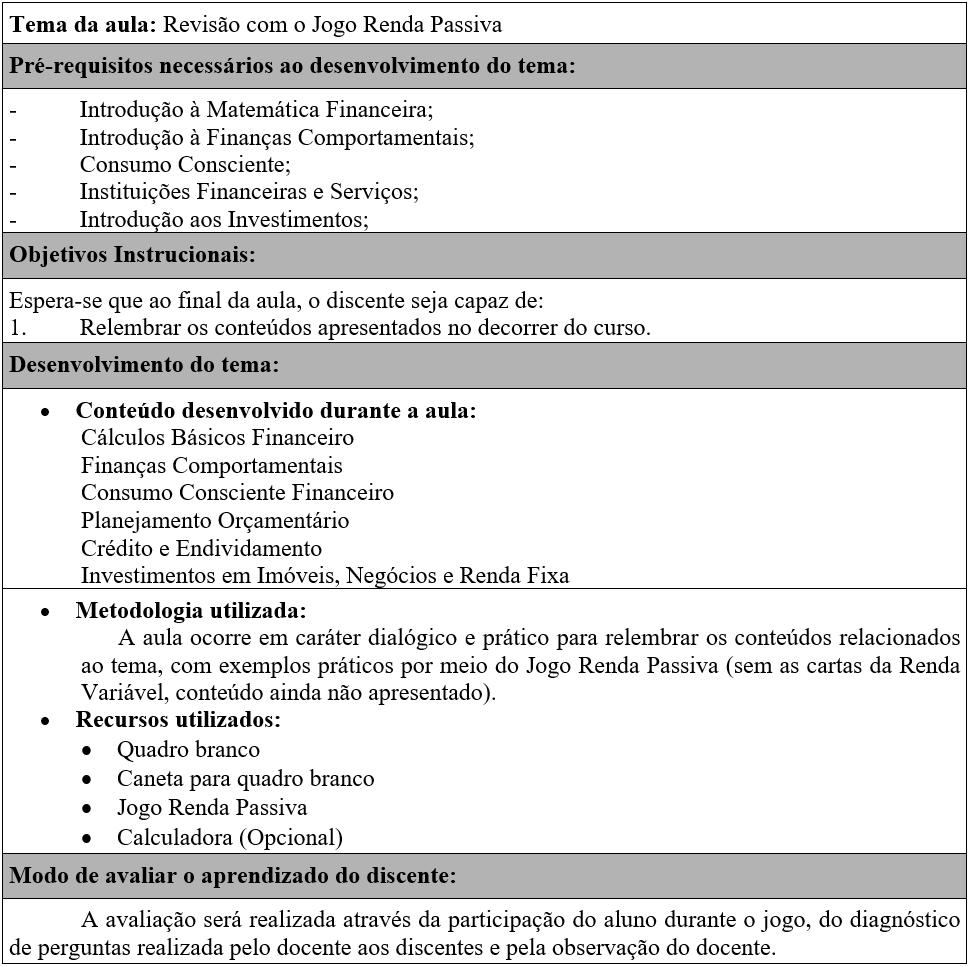
\includegraphics[width=0.9\textwidth]{quadro-12-aula 6}
\legend{\footnotesize Fonte: O autor, 2019}
\label{quad: quadro-12-aula 6}
\end{minipage}
\end{quadro}

Segundo Piccini (\citeyear{piccini2008}), a forma mais efetiva para aprendizagem através de jogos acontece quando o conteúdo a ser ensinado está dentro das regras do jogo, nesse sentido a explicação das regras do Renda Passiva pode ser considerado uma aula introdutória de educação financeira e vai ao encontro a ideia do autor, pois os elementos e normas do jogo são bem similares aos conteúdos que devem ser elucidados para os alunos.

Por esse motivo, no início desse encontro o professor deve apresentar aos alunos os elementos e regras do jogo Renda Passiva, entretanto, assimilar todas as regras de uma só vez pode ser complexo para alunos que não têm afinidade com o tema do jogo, por isso o professor deve fragmentar a explicação das regras do jogo e ilustrar inicialmente as relacionadas ao objetivo do jogo, à ficha financeira, à movimentação e ao significado dos ícones do tabuleiro, aos cenários e às cartas (exceto renda variável), elementos cruciais para o início do jogo. Após a elucidação das principais regras o docente deve retirar as cartas de variação e as cartas surpresa relacionada às ações, dividir os personagens do jogo entre os alunos a seu critério e iniciar o jogo, cada personagem e sua respectiva ficha financeira deve ser administrada um ou dois jogadores, a critério do docente. Possivelmente durante o jogo surgirão dúvidas dos alunos sobre jogabilidade que deverá ser respondida por outros colegas que já compreenderam as regras ou pelo professor. No decorrer do jogo o professor deve observar se as regras apresentadas foram compreendidas e estão sendo executadas pelos alunos e apresentar as regras conforme a necessidade. Após a assimilação do jogo por todos os alunos, o docente pode apresentar as regras acerca dos empréstimos bancário, portabilidade e limites de crédito, movimentação entre cenários por meio do aeroporto e falência do personagem, deixando as regras relacionadas às ações para os próximos encontros.

\section{7º ENCONTRO - RENDA VARIÁVEL E PREVIDÊNCIA}
O objetivo do sétimo encontro é apresentar aos estudantes os aspectos relacionados à introdução de investimentos financeiros, especificamente, em renda variável, bem como explicar o funcionamento e os tipos de previdência no Brasil. Os conteúdos relacionados a unidade temática estão descritos no quadro \ref{quad: quadro-13-aula 7} que apresenta o plano de aula do 7º encontro.
\graphicspath{{quadros/}} 
\begin{quadro}[!ht]
\centering
\begin{minipage}{0.8\textwidth}
\caption{Plano de Aula 7º Encontro}
\centering
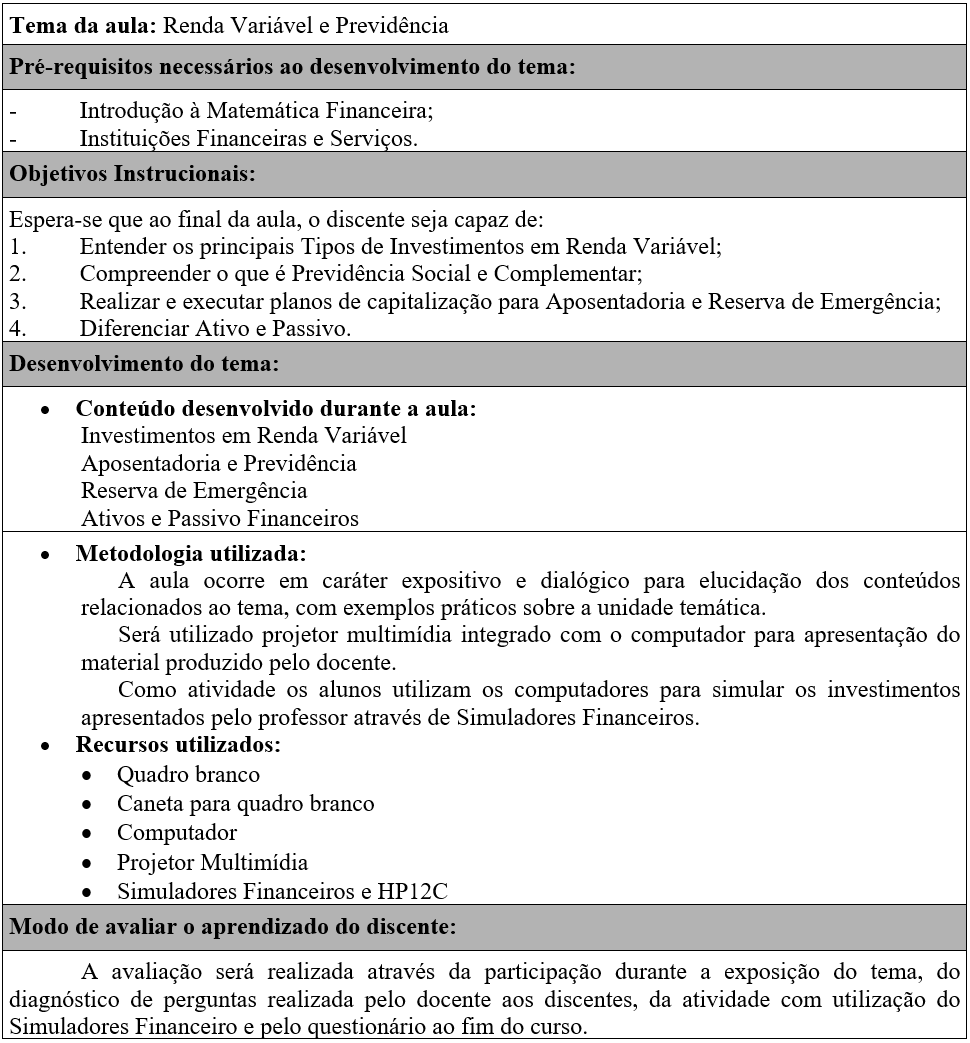
\includegraphics[width=0.9\textwidth]{quadro-13-aula 7}
\legend{\footnotesize Fonte: O autor, 2019}
\label{quad: quadro-13-aula 7}
\end{minipage}
\end{quadro}

\newpage
Esse encontro é divido em duas etapas, na primeira parte o professor deve apresentar aos alunos questões relacionadas a aposentadoria, tais como, vantagens e desvantagens dos tipos de previdência (Social e Privada), a importância de poupar recursos financeiros para a aposentadoria, os tipos de aplicações que podem ser utilizadas para aposentadoria, como o Tesouro Direto IPCA+ 2045 (https://www.tesourodireto.com.br/titulos/precos-e-taxas.htm). Após a explanação do tema da aula, os alunos realizam uma atividade de planejamento de aposentadoria, eles devem estimar o valor que desejam receber quando se aposentarem, estabelecer aportes mensais e escolher um tipo de investimento para alcançar o valor final, por intermédio de simulações financeira realizadas no simulador do tesouro direto (https://www.tesourodireto.com.br/simulador/) ou de outros tipos de aplicações a longo prazo.

Na segunda etapa o professor apresenta aos alunos conceitos introdutórios relacionados aos investimentos em renda variável, tais como, risco, rentabilidade, liquidez, ações, fundo de ações, fundos imobiliários, dividendo, valorização de ativos, taxa de custódia e de corretagem. Também deve apresentar de forma sucinta um portal e um \textit{home broker} de uma instituição de investimentos, utilizando uma conta de demonstração ou qualquer outro simulador de negociação de ativos financeiros, para que os alunos possam observar como é realizado a contratação de aplicações financeiras em renda variável através de compra e venda de ativos no mercado de ações.

Ao final deste encontro, aplicando o conhecimento adquirido e buscando estudar novos conteúdos sobre finanças, o aluno poderá alcançar o estágio Investidor Formal do desenvolvimento cognitivo do letramento financeiro, pois compreende a importância e aplica o planejamento orçamentário, busca sempre poupa recursos, realiza consumo consciente, conhece os tipos de serviços e instituições financeiras, assim como investe os recursos em diferentes aplicações de acordo com o seu perfil e objetivos financeiros.

\section{8º ENCONTRO - JOGO RENDA PASSIVA E APLICAÇÃO DOS QUESTIONÁRIOS}
O objetivo do oitavo encontro é revisar junto aos discentes todos os conteúdos abordados no curso através do jogo sério Renda Passiva, entretanto desta vez os alunos utilizam o jogo com todos os recursos e regras disponíveis. O plano de aula deste encontro está descrito no quadro \ref{quad: quadro-14-aula 8}.

\graphicspath{{quadros/}} 
\begin{quadro}[!ht]
\centering
\begin{minipage}{0.8\textwidth}
\caption{Plano de Aula 8º Encontro}
\centering
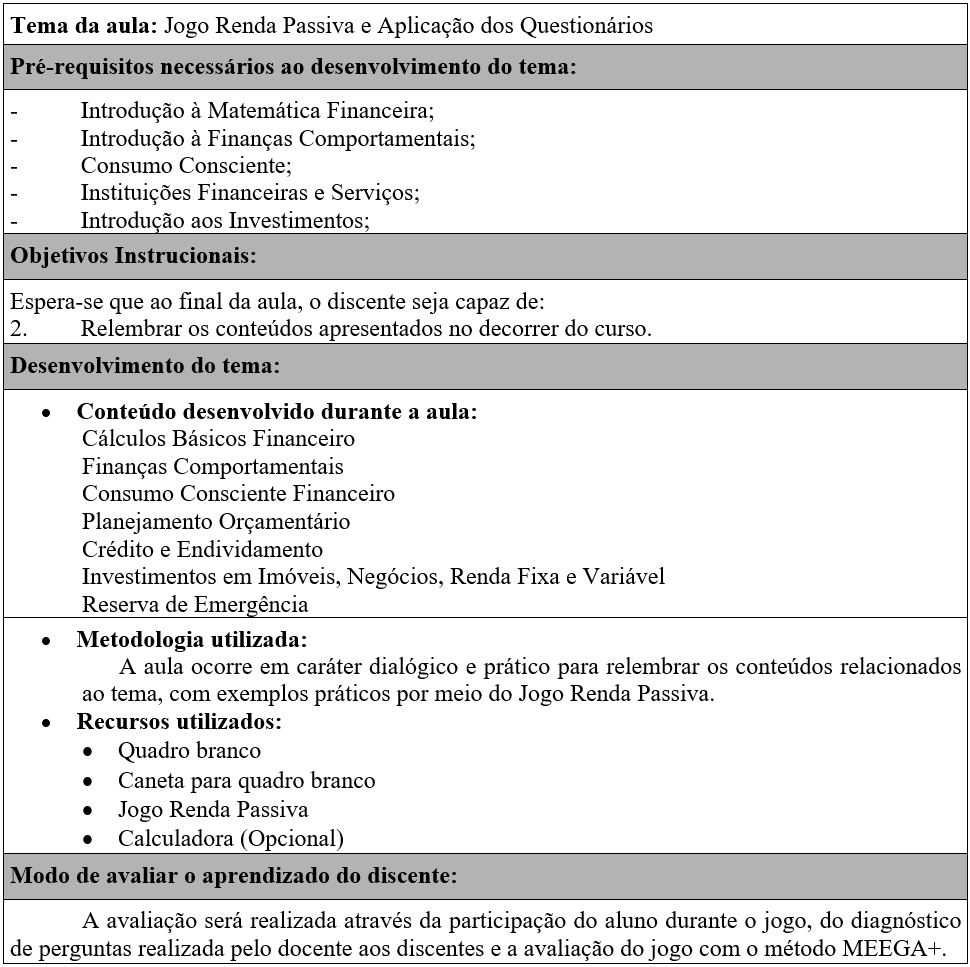
\includegraphics[width=0.9\textwidth]{quadro-14-aula 8}
\legend{\footnotesize Fonte: O autor, 2019}
\label{quad: quadro-14-aula 8}
\end{minipage}
\end{quadro}

No início do encontro o docente deve apresentar as regras do jogo que não foram apresentadas aos alunos relacionadas às ações, às cartas de variação e aos dividendos, em seguida dividir os personagens do jogo entre os alunos a seu critério e iniciar o jogo, cada personagem e sua respectiva ficha financeira deve ser administrada por um ou dois jogadores. As regras e os elementos do jogo possibilitam ao aluno colocar em prática o conhecimento adquirido durante o curso, favorecendo a aprendizagem. Normalmente nesse encontro os alunos utilizam o jogo Renda Passiva de forma mais fluida, sem tanta intervenção e interação do professor pois, os estudantes já tiveram contato com o jogo e suas regras em aulas anteriores, dessa forma o docente pode observar as atitudes dos alunos durante o jogo e realizar alguns questionamentos aos alunos, a fim de auxiliá-los nas resoluções dos problemas financeiros que o jogo disponibiliza.

\chapter{RESULTADOS E DISCUSSÕES}
O curso de “Educação Financeira através de Jogos” para ensino médio integrado do IFSUL Câmpus Gravataí ocorreu de 14/08/2019 a 27/11/2019 com duas aulas semanais. Os alunos participantes do curso, sujeitos da presente pesquisa, obtiveram uma frequência superior a 75\%, exceto uma aluna que não permaneceu até o final, pois solicitou a transferência para outra instituição, fato que indica o engajamento dos alunos no processo de aprendizagem, tendo em vista que os estudantes não eram obrigados a permanecer no curso, pois este não faz parte do projeto pedagógico do ensino médio integrado da instituição. Por isso, os dados apresentados na análise dos resultados da pesquisa consideram apenas as interações dos 18 alunos com as atividades, tarefas e questionários elaborados.

Conforme descrito nos capítulos anteriores, a avaliação dos resultados do presente projeto baseia-se em 5 instrumentos: o questionário de avaliação da aprendizagem (apêndice \ref{apend-a}), o questionário de avaliação do curso (apêndice \ref{apend-b}), o questionário de aplicação do conhecimento (apêndice \ref{apend-c}) e a avaliação dos jogos Orçamento Consciente e Renda Passiva por intermédio do método MEEGA+, com o objetivo de utilizar este método para obter dados sobre a experiência, principalmente em relação à percepção de aprendizagem do ponto de vista dos estudantes durante a utilização dos jogos.

O método avaliativo MEEGA+ possui uma seção para verificar a frequência que os sujeitos da pesquisa utilizam jogos digitais e não digitais. O resultado desse aspecto na presente pesquisa, apresentado nos gráficos \ref{graf: g2-jogos digitais} e \ref{g3-jogos não digitais}, aponta que 95\% dos estudantes que participaram do curso lidam com jogos, a maior parte utiliza jogos digitais com frequência diária ou semanal. Esse dado demonstra a familiaridade dos adolescentes da pesquisa com o mundo dos jogos, utilizar recursos ligados à experiência dos alunos favorece a aprendizagem, por isso a utilização de jogos no ensino demonstra ser um método interessante que pode ser usado pelos professores no ensino da educação financeira.

\graphicspath{{graficos/}} 
\begin{grafico}[!ht]
\centering
\begin{minipage}{0.9\textwidth}
\caption{Frequência de Utilização de Jogos Digitais pelos Estudantes}
\centering
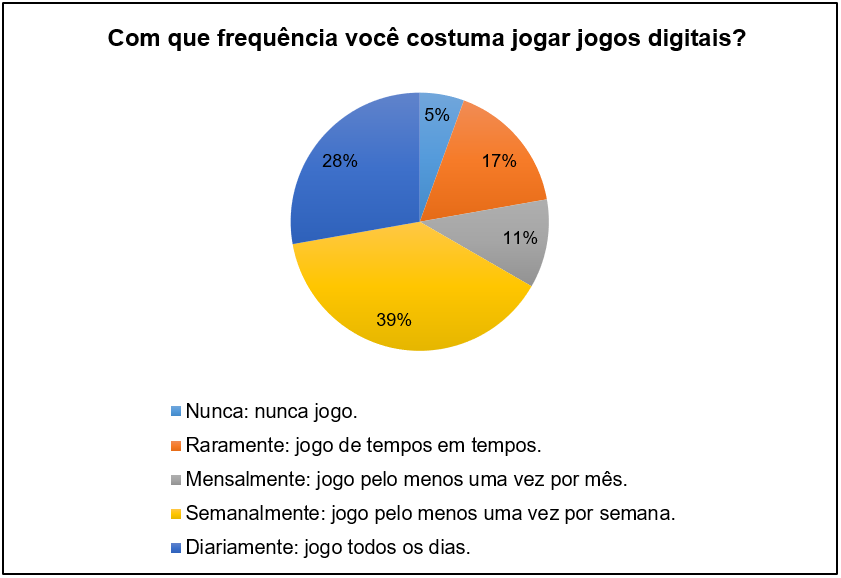
\includegraphics[width=0.9\textwidth]{g2-jogos digitais}
\legend{\footnotesize Fonte: Dados da pesquisa. Adaptado de Petri (\citeyear{petri2017})}
\label{graf: g2-jogos digitais}
\end{minipage}
\end{grafico}

\graphicspath{{graficos/}} 
\begin{grafico}[!ht]
\centering
\begin{minipage}{0.9\textwidth}
\caption{Frequência de Utilização de Jogos Não Digitais pelos Estudantes}
\centering
\includegraphics[width=0.9\textwidth]{g3-jogos não digitais}
\legend{\footnotesize Fonte: Dados da pesquisa. Adaptado de Petri (\citeyear{petri2017})}
\label{graf: g3-jogos não digitais}
\end{minipage}
\end{grafico}

\newpage
Os demais resultados da análise dos dados alcançados com os questionários do MEEGA+ para avaliar a aprendizagem por meio dos jogos Orçamento Consciente e Renda Passiva, a retenção dos assuntos abordados, a eficiência do curso “Educação Financeira através de Jogos”, a utilização do conhecimento adquirido e para verificar os estágios do desenvolvimento cognitivo do letramento financeiro dos alunos estão descritos nos subitens a seguir no presente capítulo.

\section{ANÁLISE DOS RESULTADOS DO JOGO ORÇAMENTO CONSCIENTE}
Os relatos sobre a experiência dos estudantes na interação com o jogo Orçamento Consciente foram levantados com a aplicação do método avaliativo MEEGA+. As perguntas deste método e os dados coletados com as respostas dos discentes estão expostos no gráfico \ref{graf: g4-experiência-orçamento} (experiência do jogador) e no gráfico 5 (usabilidade do jogo), bem como os pontos fortes no quadro 15, as sugestões de melhoria no quadro \ref{quad: quadro-16-Melhorias - Jogo Orçamento Consciente} e os comentários adicionais acerca do jogo no quadro \ref{quad: quadro-17-Comentário Adicionais - Jogo Orçamento Consciente}.

\graphicspath{{graficos/}} 
\begin{grafico}[!ht]
\centering
\begin{minipage}{0.9\textwidth}
\caption{Avaliação do Jogo Orçamento Consciente (Experiência)}
\centering
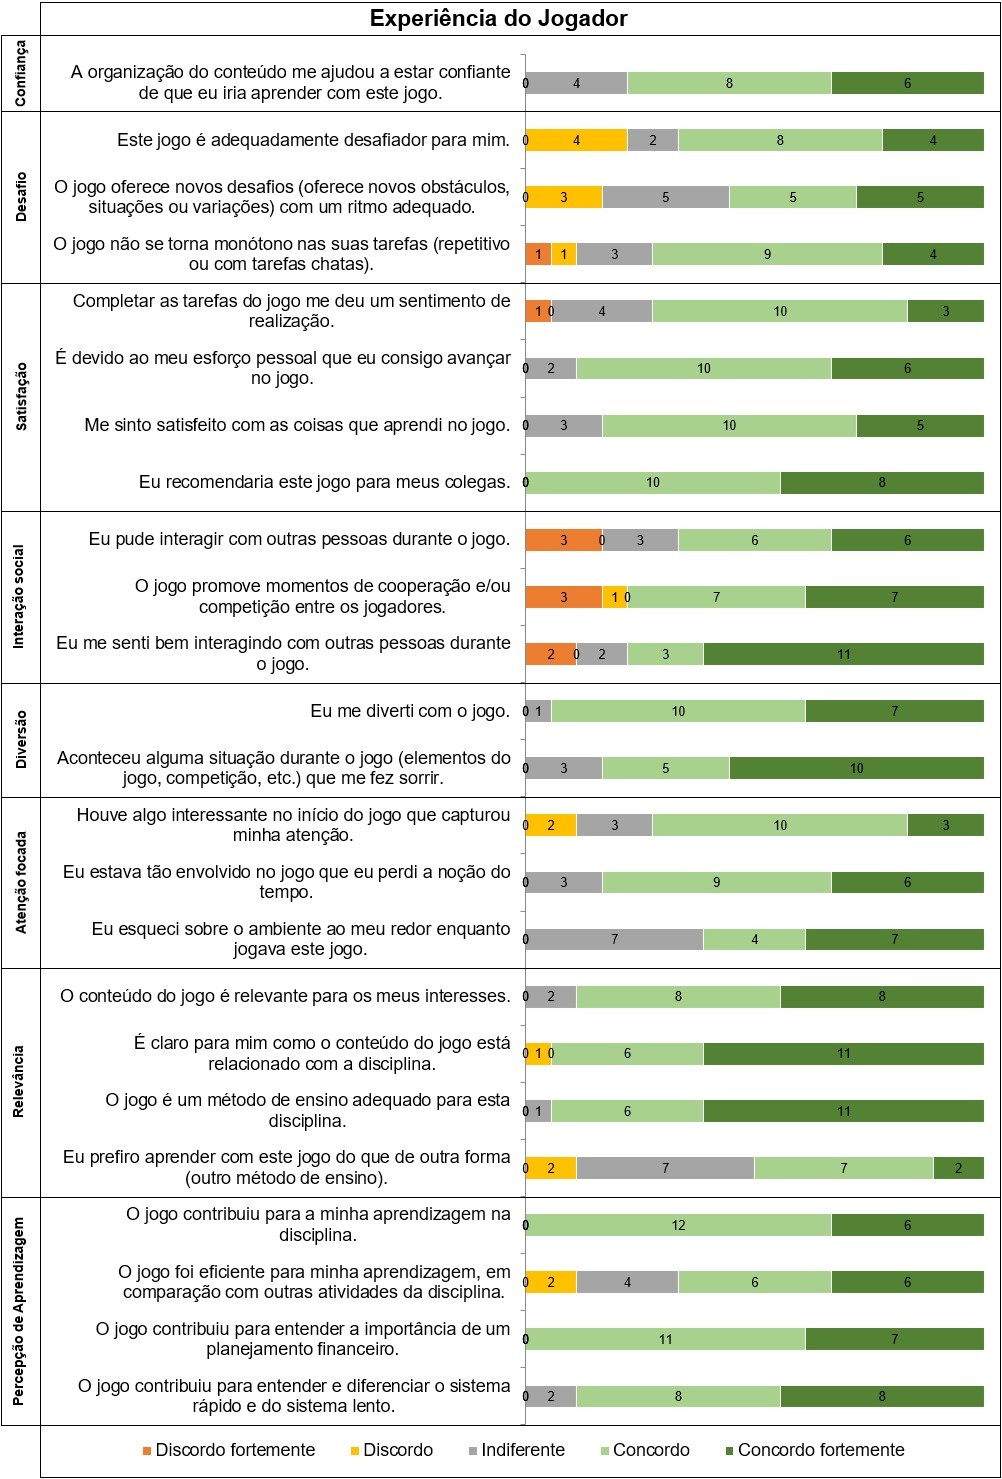
\includegraphics[width=0.9\textwidth]{g4-experiência-orçamento}
\legend{\footnotesize Fonte: Dados da pesquisa. Adaptado de Petri (\citeyear{petri2017})}
\label{graf: g4-experiência-orçamento}
\end{minipage}
\end{grafico}

Os resultados acerca da experiência do jogador revelam que os aspectos necessários para melhoria do jogo Orçamento Consciente estão relacionados ao “Desafio” e à “Interação social” (concentração de cores laranja e amarelo do gráfico \ref{graf: g4-experiência-orçamento}), abrindo margem para a hipótese de que a falta de incentivo à interação entre os jogadores, bem como de uma progressão de desafios mais adequada, pode ter influenciado no engajamento por parte dos alunos. Uma possível interpretação destes resultados pode sugerir que a atenção dos jogadores reduziu à medida que aprenderam a utilizar da forma lenta de pensar para cumprir com os objetivos, tornando o restante do jogo pouco desafiador para alguns.

Em relação aos aspectos positivos na experiência da interação dos alunos com o jogo Orçamento Consciente, pode-se destacar que todos os sujeitos da pesquisa relataram que o jogo contribuiu para a aprendizagem da disciplina e na compreensão da importância do planejamento financeiro, relatos observados no aspecto da “Percepção de Aprendizagem” no gráfico \ref{graf: g4-experiência-orçamento}, os estudantes declararam também que recomendariam o jogo aos outros colegas (gráfico \ref{graf: g4-experiência-orçamento} - Satisfação). Outrossim, a maioria dos estudantes participantes do curso relataram que:

\begin{itemize}
    \item o jogo contribuiu para entender e diferenciar o pensamento rápido e do lento, propostos por Kahneman (\citeyear{kahneman2012});

    \item a organização do conteúdo os ajudou a adquirir confiança para aprender com o jogo (gráfico \ref{graf: g4-experiência-orçamento} - Confiança);

    \item se sentiram satisfeitos com o conhecimento adquirido por intermédio do jogo (gráfico \ref{graf: g4-experiência-orçamento} - Satisfação) e se divertiram ao jogar (gráfico \ref{graf: g4-experiência-orçamento} - Diversão);

    \item estavam tão envolvidos no jogo que perderam a noção do tempo (gráfico \ref{graf: g4-experiência-orçamento} - Atenção Focada);

    \item o jogo é adequado, relevante e dispõe de conteúdos relacionados com a disciplina (gráfico \ref{graf: g4-experiência-orçamento} - Relevância).
\end{itemize}

Em relação à usabilidade do jogo, representado no gráfico \ref{graf: g5-usabilidade-orçamento}, os dados apontam que para a maior parcela dos estudantes foi fácil entender as regras e aprender a jogar o Orçamento Consciente, da mesma maneira que o jogo possui fontes legíveis e cores compreensíveis, entretanto alguns alunos não consideram o jogo fácil e foram indiferentes com o design (combinação cores, textos e fontes) do jogo, aspectos observado no gráfico \ref{graf: g5-usabilidade-orçamento} nos tópicos “Estética” e “Operabilidade”, o que sugere indicação de possíveis melhorias nestes aspectos do jogo.

\graphicspath{{graficos/}} 
\begin{grafico}[!ht]
\centering
\begin{minipage}{0.9\textwidth}
\caption{Avaliação do Jogo Orçamento Consciente (Usabilidade)}
\centering
\includegraphics[width=0.9\textwidth]{g5-usabilidade-orçamento}
\legend{\footnotesize Fonte: Dados da pesquisa. Adaptado de Petri (\citeyear{petri2017})}
\label{graf: g5-usabilidade-orçamento}
\end{minipage}
\end{grafico}

Os pontos fortes do jogo Orçamento Consciente descritos pelos alunos e exibidos no quadro \ref{quad: quadro-15-Pontos Fortes - Jogo Orçamento Consciente}, nota-se relatos acerca do pensamento rápido, gatilhos mentais, comportamento financeiro e compreensão da disciplina como pontos fortes do jogo, há também elogio à construção do jogo, à dinâmica, às imagens e à metodologia utilizada na construção do jogo.

\graphicspath{{quadros/}} 
\begin{quadro}[!ht]
\centering
\begin{minipage}{0.8\textwidth}
\caption{Jogo Orçamento Consciente (Pontos Fortes)}
\centering
\includegraphics[width=0.9\textwidth]{quadro-15-Pontos Fortes - Jogo Orçamento Consciente}
\legend{\footnotesize Fonte: Dados da pesquisa}
\label{quad: quadro-15-Pontos Fortes - Jogo Orçamento Consciente}
\end{minipage}
\end{quadro}

Os relatos dos alunos no quadro \ref{quad: quadro-15-Pontos Fortes - Jogo Orçamento Consciente} e na “Percepção de Aprendizagem” (gráfico \ref{graf: g4-experiência-orçamento}) confirmam a hipótese que a utilização deste jogo sério facilitou o processo de aprendizagem e satisfação dos discentes, assim como sugerem que a ideia dos desenvolvedores do jogo Orçamento Consciente foi adequadamente expressa e percebida pelos jogadores. Tendo em vista que a ideia norteadora durante o desenvolvimento do projeto foi produzir um ambiente no qual o jogador precisasse lidar com sua forma rápida de pensar, inibindo os gatilhos mentais e realizando um consumo consciente a fim de se obter mais recompensas. Desta forma, o jogo Orçamento Consciente alcançou o objetivo proposto, pois, favoreceu a aprendizagem dos alunos sobre as finanças comportamentais, a importância do planejamento orçamentário e a nossa relação com o dinheiro, conhecimentos necessários para que o sujeito ascenda ao estágio Consumidor Pré-Poupador do desenvolvimento cognitivo do letramento financeiro.

Na seção de sugestões de melhorias do questionário MEEGA+ (quadro \ref{quad: quadro-16-Melhorias - Jogo Orçamento Consciente}), os relatos dos estudantes apontam para ampliação do jogo, para que este possa disponibilizar informações e sugestões de planejamento financeiro, recompensas maiores por aplicar um bom planejamento, adicionar mais opções de produtos e adicionar outros elementos ao jogo, também sugeriram melhorar o \textit{layout} e aumento no tempo para compras. Dois estudantes apontaram nesta seção uma percepção que o jogo disponibiliza poucos produtos relacionados à saúde, circunstância colocada propositalmente pelos desenvolvedores, pois, no planejamento do jogo procurou-se refletir o orçamento financeiro no qual o gasto com alimentação e compras é maior do que os gastos com saúde.

\graphicspath{{quadros/}} 
\begin{quadro}[!ht]
\centering
\begin{minipage}{0.8\textwidth}
\caption{Jogo Orçamento Consciente (Sugestões de Melhoria)}
\centering
\includegraphics[width=0.9\textwidth]{quadro-16-Melhorias - Jogo Orçamento Consciente}
\legend{\footnotesize Fonte: Dados da pesquisa}
\label{quad: quadro-16-Melhorias - Jogo Orçamento Consciente}
\end{minipage}
\end{quadro}

Quanto aos comentários adicionais do questionário MEEGA+ (quadro \ref{quad: quadro-17-Comentário Adicionais - Jogo Orçamento Consciente}), apenas 6 alunos responderam esta seção, na maior parte das respostas os alunos elogiaram o jogo e o curso, somente um estudante indicou uma melhoria, também no sentido de ampliação para que o este forneça direcionamento ao jogador.

\graphicspath{{quadros/}} 
\begin{quadro}[!ht]
\centering
\begin{minipage}{0.8\textwidth}
\caption{Jogo Orçamento Consciente (Comentários Adicionais)}
\centering
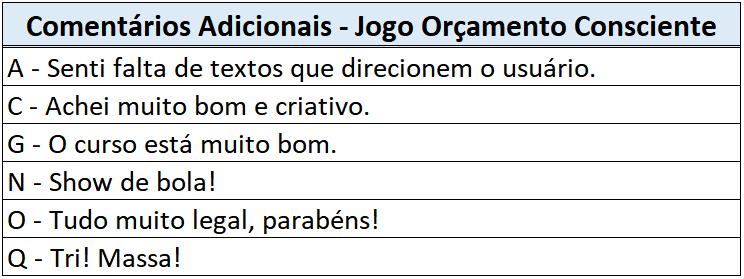
\includegraphics[width=0.85\textwidth]{quadro-17-Comentário Adicionais - Jogo Orçamento Consciente}
\legend{\footnotesize Fonte: Dados da pesquisa}
\label{quad: quadro-17-Comentário Adicionais - Jogo Orçamento Consciente}
\end{minipage}
\end{quadro}

\newpage
Por intermédio dos relatos nos pontos fortes, nas sugestões de melhoria, nos comentários adicionais e na experiência dos alunos na interação com o jogo Orçamento Consciente observa-se que o jogo sério foi bem recebido pelos alunos no processo de ensino-aprendizagem, favorecendo a compreensão da introdução de finanças comportamentais, consumo consciente e orçamento. As melhorias sugestionadas pelos participantes da pesquisa devem ser aplicadas no jogo Orçamento Consciente para proporcionar maior qualidade ao jogo e, consequentemente, ao processo de aprendizagem dos estudantes.

\section{ANÁLISE DOS RESULTADOS DO JOGO RENDA PASSIVA}
Os relatos sobre a experiência dos estudantes na interação com o jogo Renda Passiva foram levantados com a aplicação parcial do método avaliativo MEEGA+, aplicar este jogo exige um período grande da aula, por isso optou-se por utilizar somente as indagações mais cruciais do questionário em relação do objetivo deste estudo, principalmente as questões relacionadas à aprendizagem. As perguntas do método MEEGA+ e os dados coletados com as respostas dos discentes estão expostos no gráfico \ref{graf: g6-experiencia-renda-passiva} (experiência do jogador), bem como os pontos fortes no quadro \ref{quad: quadro-18-pontos fortes-renda-passiva}, as sugestões de melhoria no quadro \ref{quad: quadro-19-sugestões de melhoria-renda-passiva} e os comentários adicionais acerca do jogo no quadro \ref{quad: quadro-20-comentários adicionais-renda-passiva}.

\graphicspath{{graficos/}} 
\begin{grafico}[!ht]
\centering
\begin{minipage}{0.9\textwidth}
\caption{Avaliação do Jogo Renda Passiva (Experiência)}
\centering
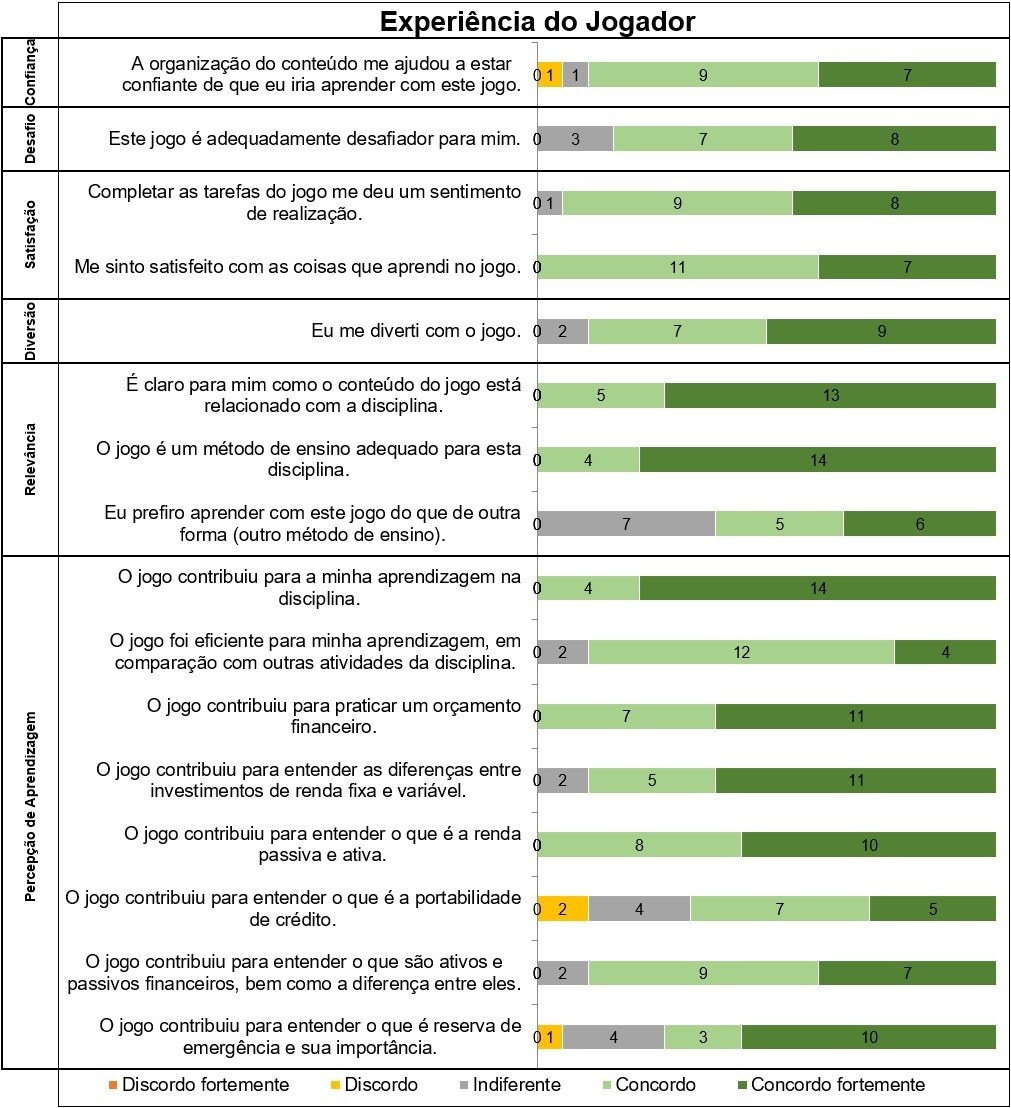
\includegraphics[width=0.9\textwidth]{g6-experiencia-renda-passiva}
\legend{\footnotesize Fonte: Dados da pesquisa. Adaptado de Petri (\citeyear{petri2017})}
\label{graf: g6-experiencia-renda-passiva}
\end{minipage}
\end{grafico}

\newpage
Em relação aos aspectos positivos na experiência da interação dos alunos com o jogo Renda Passiva, pode-se destacar que todos os sujeitos da pesquisa relataram satisfação com o conhecimento adquirido durante o jogo, sendo ele adequado para a disciplina e relacionado com o tema estudado, relatos observados nos aspectos “Satisfação” e “Relevância” da gráfico \ref{graf: g6-experiencia-renda-passiva}, bem como relataram no aspecto “Percepção de Aprendizagem” que o jogo contribuiu para aprendizagem da disciplina, para praticar um orçamento financeiro e para compreender o conceito de renda passiva e renda ativa. Outrossim, a maioria dos estudantes participantes do curso “Educação Financeira através de Jogos” relataram que:

\begin{itemize}
    \item a organização do conteúdo os ajudou a adquirir confiança para aprender com o jogo (gráfico \ref{graf: g6-experiencia-renda-passiva} - Confiança);

    \item o jogo é adequadamente desafiador, divertido (gráfico \ref{graf: g6-experiencia-renda-passiva} - Diversão e Desafio) e eficiente para a aprendizagem (gráfico \ref{graf: g6-experiencia-renda-passiva} - Percepção de Aprendizagem);

    \item o jogo contribuiu para entender a diferença entre investimentos de renda fixa e variável, portabilidade de crédito, o que são ativos e passivos financeiros e a importância da reserva de emergência.
\end{itemize}

O resultado na análise dos aspectos referentes à “Percepção de Aprendizagem”, exibido no gráfico \ref{graf: g6-experiencia-renda-passiva}, demonstra que o jogo Renda Passiva favoreceu a aprendizagem dos conteúdos da disciplina. Entretanto, uma parcela pequena dos alunos relataram que o jogo não contribuiu para aprendizagem, principalmente acerca da portabilidade de crédito e da importância da reserva de emergência (concentração de cores cinza e amarelo do gráfico \ref{graf: g6-experiencia-renda-passiva}). Uma possível interpretação deste resultado pode sugerir que as soluções escolhidas por esses alunos, para resolver problemas financeiros propostos, influencia diretamente na aprendizagem. Desta forma, o jogador vai assimilar melhor os conteúdos que se apresentam no caminho que decidiu percorrer no jogo em detrimento a outros, como exemplo, ele pode decidir quitar os empréstimos apenas poupando e aplicando o salário, ao invés de realizar a portabilidade de crédito para um juros menor, nesse caso o jogador não possuirá interação com um novo crédito e pode não perceber a contribuição de tal instrumento financeiro no jogo. Por isso, é importante que os alunos tenham diversas interações com o jogo, pois a cada partida o Renda Passiva oferece dificuldades financeiras distinta, instigando o jogador usar instrumentos diferentes para cada desafio, assim, o estudante poderá interagir com todos os aspectos do jogo favorecendo a aprendizagem dos diversos conteúdos.

O resultado na análise dos pontos fortes do jogo Renda Passiva, expostos pelos alunos e exibidas no quadro \ref{quad: quadro-18-pontos fortes-renda-passiva}, sugere que o jogo é divertido, facilita a aprendizagem e a compreensão dos temas referente ao mercado financeiro, ao planejamento orçamentário, aos investimentos e aos riscos de forma prática e lúdica. Os relatos dos estudantes sobre os pontos fortes do jogo (quadro \ref{quad: quadro-18-pontos fortes-renda-passiva}) e o tópico “Percepção de Aprendizagem” (exibida no gráfico \ref{graf: g6-experiencia-renda-passiva}) confirmam a hipótese que a utilização deste jogo facilitou o processo de aprendizagem. Desta forma, mesmo sendo um jogo de entretenimento, ele pode ser utilizado como jogo sério utilizado para auxiliar os professores no processo de ensino da educação financeira, dirimindo a complexidade do conteúdo estudado, facilitando o entendimento dos alunos e favorecendo a aprendizagem de finanças.

\graphicspath{{quadros/}} 
\begin{quadro}[!ht]
\centering
\begin{minipage}{0.8\textwidth}
\caption{Jogo Renda Passiva (Pontos Fortes)}
\centering
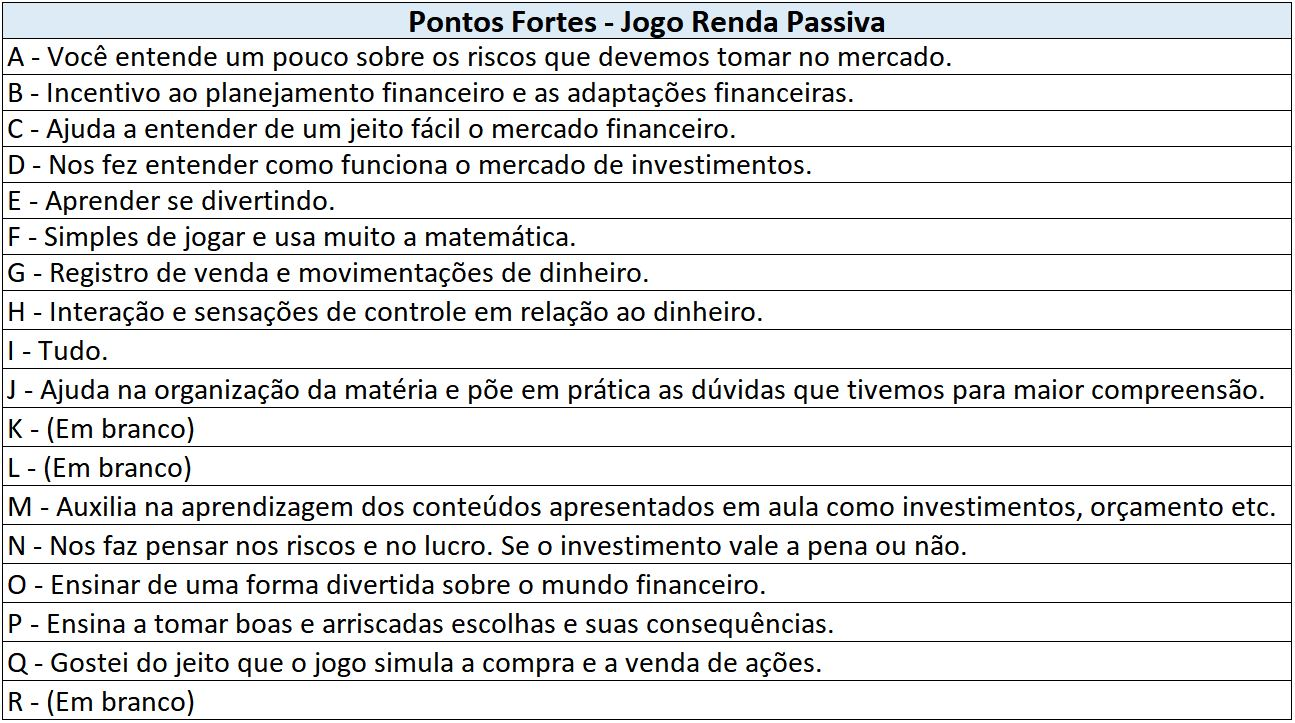
\includegraphics[width=0.85\textwidth]{quadro-18-pontos fortes-renda-passiva}
\legend{\footnotesize Fonte: Dados da pesquisa}
\label{quad: quadro-18-pontos fortes-renda-passiva}
\end{minipage}
\end{quadro}

\newpage
Na seção de sugestões de melhorias do questionário MEEGA+ (quadro \ref{quad: quadro-19-sugestões de melhoria-renda-passiva}), os alunos relataram que o jogo Renda Passiva poderia utilizar tecnologias para cálculos do registro financeiro e valores reais do mercado financeiro nas taxas, assim como, disponibilizar um tempo maior para jogar e instruções mais clara sobre as regras do jogo para apoio dos jogadores.

\graphicspath{{quadros/}} 
\begin{quadro}[!ht]
\centering
\begin{minipage}{0.8\textwidth}
\caption{Jogo Renda Passiva (Sugestões de Melhoria)}
\centering
\includegraphics[width=0.85\textwidth]{quadro-19-sugestões de melhoria-renda-passiva}
\legend{\footnotesize Fonte: Dados da pesquisa}
\label{quad: quadro-19-sugestões de melhoria-renda-passiva}
\end{minipage}
\end{quadro}

Considerando as sugestões de melhoria propostas pelos alunos (quadro \ref{quad: quadro-19-sugestões de melhoria-renda-passiva}), o presente autor acredita que utilizar a tecnologia inicialmente pode desfavorecer a prática de cálculos matemáticos relacionados às finanças, outro fator importante é que o mercado financeiro é extremamente dinâmico, por isso para implementar taxas e indexadores reais sobre finanças em um jogo de tabuleiro pode ser complicado, além de dificultar a operabilidade do jogo, entretanto é algo interessante de propor. Outro fato relevante de esclarecer é que o mercado financeiro possui muitos regulamentos, desta forma, segundo Piccini (\citeyear{piccini2008}), um jogo que tem o objetivo ensinar educação financeira precisa ter diretrizes semelhantes ao mercado financeiro, por esse motivo o jogo Renda Passiva possui muitos conceitos e regras, se comparados à outros jogos financeiros, entretanto, o jogo representa fielmente características financeira pessoal e familiar, provavelmente, a falta de proximidade com a temática do jogo causam dificuldades em alguns alunos para compreender as regras, mesmo assim apenas dois alunos relataram tais dificuldades e sentiram falta de mais orientações, contudo, os docentes que utilizarem o jogo podem aplicar os regramentos do Renda Passiva gradativamente em suas aulas caso sintam necessidade. Outrossim, nota-se também nos relatos dos alunos que estes gostariam de utilizar o jogo por um tempo maior, contudo durante o curso “Educação Financeira através de Jogos” o jogo foi utilizado em um pequeno período das aulas, seu prolongamento poderia sobrepor a outras tecnologias também importantes no ensino e algumas partidas do Renda Passiva podem demorar muito mais que o horário de aula, por isso seria importante também disponibilizar o jogo aos alunos no contraturno, como forma de continuação e revisão dos estudos sobre finanças. Durante a presente pesquisa os estudantes utilizaram o jogo com todas as regras apenas uma vez no último encontro, provavelmente os relatos apontados pelos alunos indicam que eles gostariam de ter mais tempo disponibilizado durante a aula para realizar diversas partidas do jogo.

Quanto aos comentários adicionais relatados pelos alunos, por meio da resposta no questionário do MEEGA+ (quadro \ref{quad: quadro-20-comentários adicionais-renda-passiva}), apenas 3 estudantes responderam esta seção, dois estudantes elogiaram o jogo e o curso e somente um indicou uma melhoria, no sentido de ampliação do tempo de uso do jogo durante a aula.

\graphicspath{{quadros/}} 
\begin{quadro}[!ht]
\centering
\begin{minipage}{0.8\textwidth}
\caption{Jogo Renda Passiva (Comentários Adicionais)}
\centering
\includegraphics[width=0.85\textwidth]{quadro-20-comentários adicionais-renda-passiva}
\legend{\footnotesize Fonte: Dados da pesquisa}
\label{quad: quadro-20-comentários adicionais-renda-passiva}
\end{minipage}
\end{quadro}

Por intermédio dos relatos nos pontos fortes, nas sugestões de melhoria, nos comentários adicionais e na experiência dos alunos na interação com o jogo Renda Passiva observa-se que o jogo foi bem recebido pelos alunos no processo de ensino, favorecendo a aprendizagem dos discentes. Este resultado indica que o jogo pode ser utilizado nas aulas de introdução à educação financeira como ferramenta prática no ensino de orçamento financeiro, investimentos e riscos, ativos e passivos, finanças comportamentais, renda passiva e ativa, reserva de emergência, portabilidade de crédito, consumo consciente, porcentagem, juros, receitas e dívidas.

\section{ANÁLISE DOS RESULTADOS DA AVALIAÇÃO DE APRENDIZAGEM}
No intuito de aferir o nível de retenção dos alunos sobre temas principais apresentados no curso, os autores da presente pesquisa elaboraram e aplicaram o questionário de Avaliação de Aprendizagem (apêndice \ref{apend-a}), com perguntas sobre conceitualização da educação e matemática financeira, orçamento financeiro, consumo consciente, juros, inflação e investimentos. As respostas dos alunos, coletadas por meio do questionário impresso, foram agrupadas para facilitar a investigação do resultado. Deste modo, o quadro \ref{quad: quadro-21-Respostas  pergunta1} apresenta o retorno da questão 1, o quadro \ref{quad: quadro-22-Respostas  pergunta2} da questão 2, assim como as questões objetivas e dissertativas estão apresentadas no gráfico \ref{graf: g7-avaliação-aprendizagem-resultado-questão}, reunidas por perguntas e no gráfico \ref{graf: g8-avaliacao-aprendizagem-resultado-aluno}, por aluno.

\graphicspath{{quadros/}} 
\begin{quadro}[!ht]
\centering
\begin{minipage}{0.8\textwidth}
\caption{Avaliação da Aprendizagem (Respostas da Questão 1)}
\centering
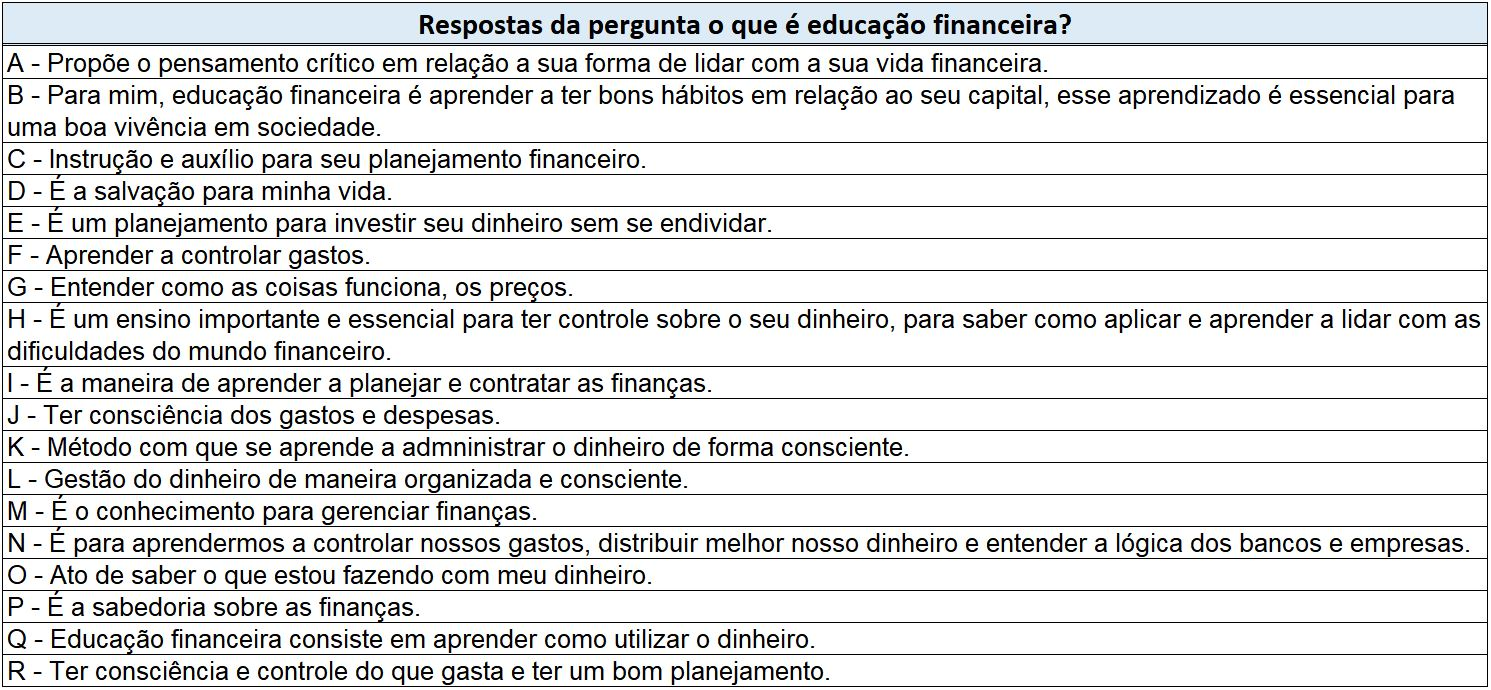
\includegraphics[width=0.85\textwidth]{quadro-21-Respostas pergunta1.JPG}
\legend{\footnotesize Fonte: Dados da pesquisa}
\label{quad: quadro-21-Respostas  pergunta1}
\end{minipage}
\end{quadro}

Segundo a OECD (\citeyear{oecd2005}), a educação financeira trata sobre a aquisição do conhecimento sobre o comportamento, emoções, hábitos e controle relacionados à vida financeira. De acordo com esta definição, considera-se que 13 alunos responderam de forma semelhante ao conceito utilizado pela OECD, o que corresponde a aproximadamente 72\% dos discentes, este dado indica que a maior parte dos sujeitos da pesquisa compreenderam o que é a educação financeira.

\graphicspath{{quadros/}} 
\begin{quadro}[!ht]
\centering
\begin{minipage}{0.8\textwidth}
\caption{Avaliação da Aprendizagem (Respostas da Questão 2)}
\centering
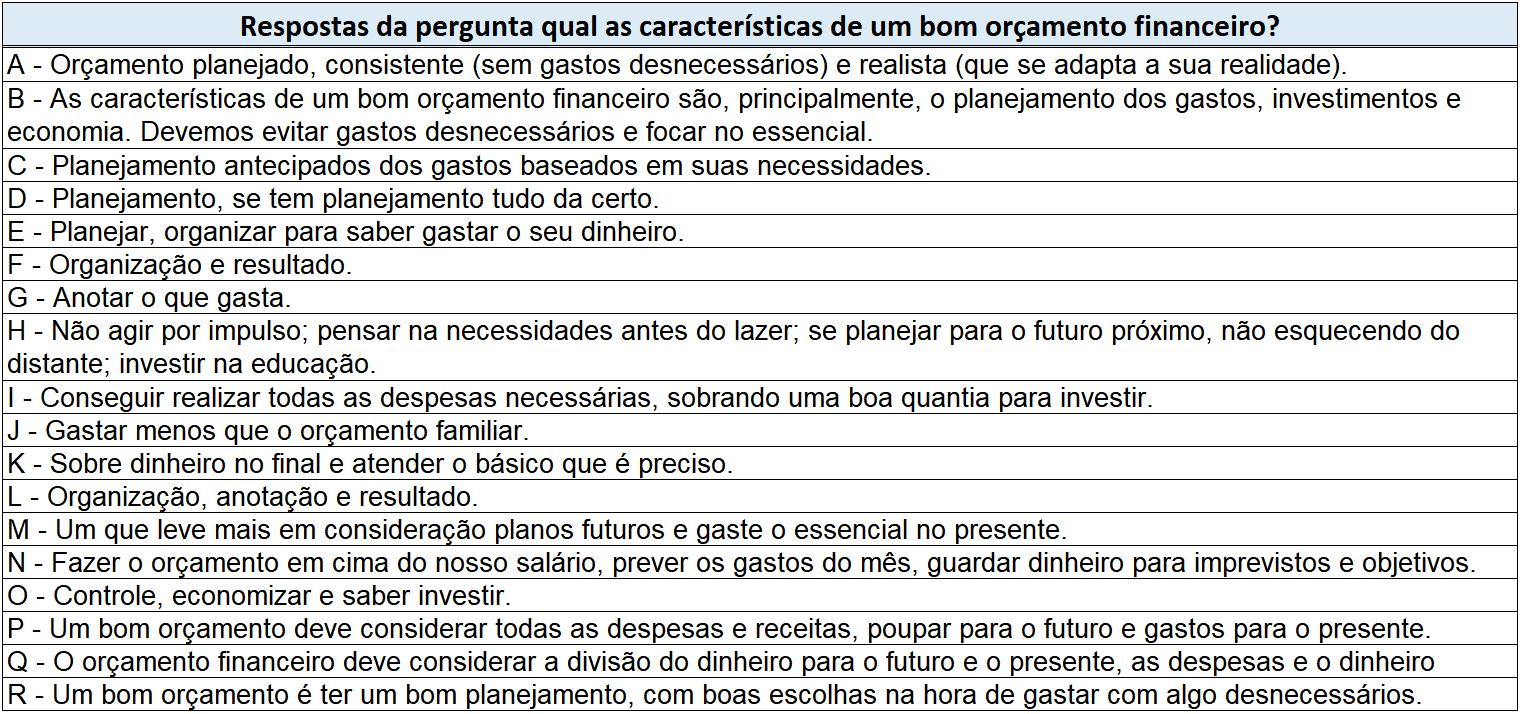
\includegraphics[width=0.85\textwidth]{quadro-22-Respostas-pergunta2}
\legend{\footnotesize Fonte: Dados da pesquisa}
\label{quad: quadro-22-Respostas  pergunta2}
\end{minipage}
\end{quadro}

Um orçamento financeiro deve conter uma lista detalhada de todas as receitas e despesas do mês, para reduzir o consumo desnecessário, manter o equilíbrio entre ganhos, gastos e poder poupar parte do dinheiro. (BUAES, COMERLATO e DOLL, \citeyear{buaes2015}; BACEN, \citeyear{bacen2013}). Considerando este conceito, nota-se no quadro \ref{quad: quadro-22-Respostas  pergunta2} que 12 alunos responderam corretamente à questão 2, aproximadamente 66\% dos discentes, este dado indica que a maior parcela dos sujeitos da pesquisa compreendeu as características e o funcionamento de um orçamento financeiro.

O gráfico \ref{graf: g7-avaliação-aprendizagem-resultado-questão} foi elaborado com o objetivo de agrupar por questão as respostas dos alunos, no intuito de verificar as dificuldades e o desempenho dos estudantes em cada uma das questões do questionário de Avaliação de Aprendizagem (apêndice \ref{apend-a}). Analisando as respostas do gráfico \ref{graf: g7-avaliação-aprendizagem-resultado-questão} é possível observar que todas as questões propostas tiveram no mínimo 60\% de respostas corretas, as perguntas que obtiveram maior quantidade de acerto foram as questões 5 (sobre consumo consciente), 7 e 11 (acerca de investimentos), as perguntas com menor quantidade de respostas corretas foram as relacionadas ao orçamento (questões 4 e 6) e à liquidez (questão 9), com apenas 11 acertos.

\graphicspath{{graficos/}} 
\begin{grafico}[!ht]
\centering
\begin{minipage}{0.8\textwidth}
\caption{Avaliação da Aprendizagem - Resultado por Questão}
\centering
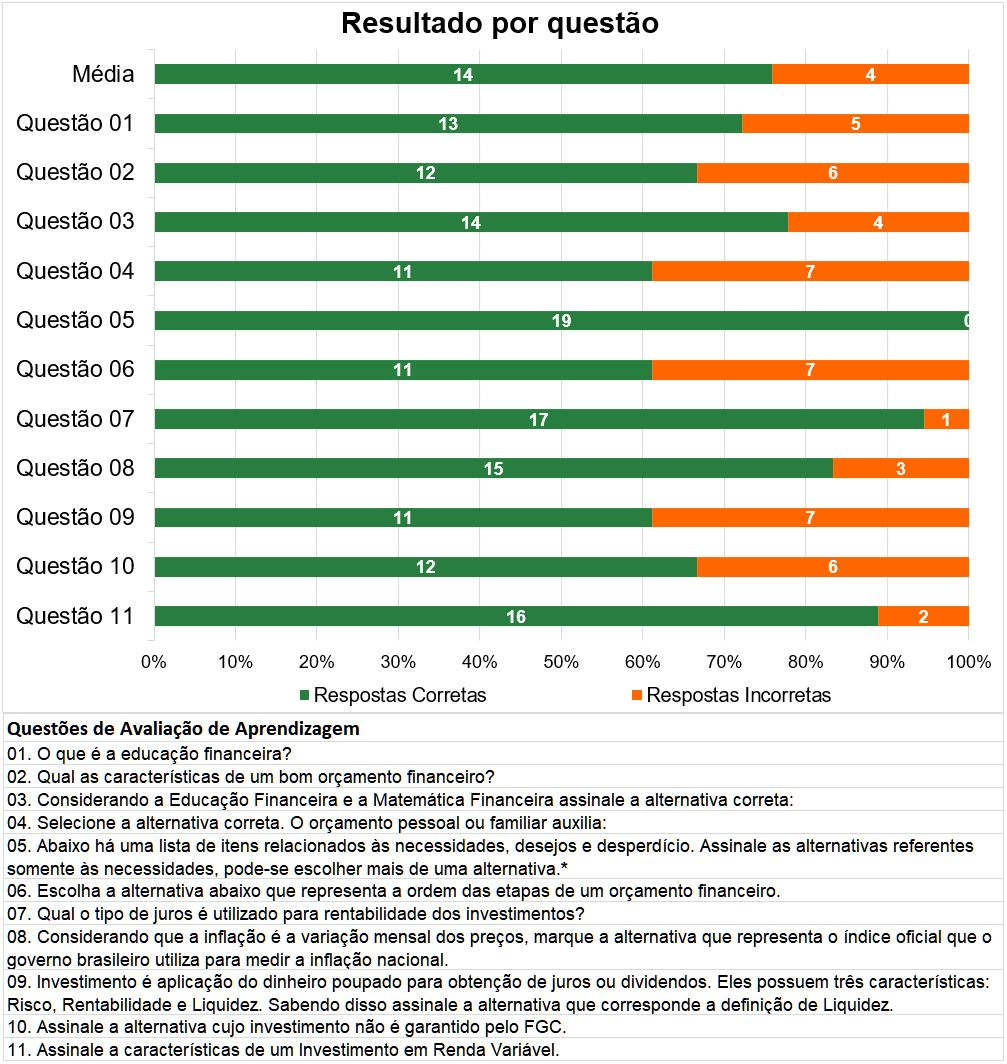
\includegraphics[width=0.9\textwidth]{g7-avaliação-aprendizagem-resultado-questão}
\footnotemark\footnotesize * Apenas um aluno escolheu mais de uma alternativa.
\legend{\footnotesize Fonte: Dados da pesquisa.}
\label{graf: g7-avaliação-aprendizagem-resultado-questão}
\end{minipage}
\end{grafico}

Percebe-se, portanto, no gráfico \ref{graf: g7-avaliação-aprendizagem-resultado-questão} e nos dados apresentados na avaliação dos jogos que a maior parcela dos alunos conseguiu compreender bem o conceito de consumo consciente e investimentos, entretanto, alguns tiveram mais dificuldades em externar conceitos relacionados ao orçamento financeiro. De modo geral, os alunos obtiveram um nível bom de respostas corretas em cada uma das perguntas o que indica uma boa retenção dos assuntos apresentados no curso.

A produção do gráfico \ref{graf: g8-avaliacao-aprendizagem-resultado-aluno} tem o objetivo de agrupar as respostas corretas e incorretas dos alunos para verificar as dificuldades e o desempenho de cada um dos estudantes nas questões do questionário de Avaliação de Aprendizagem (apêndice A). Por intermédio da análise dos resultados no gráfico \ref{graf: g8-avaliacao-aprendizagem-resultado-aluno}, é possível observar que apenas dois alunos obtiveram desempenho inferior a 50\% e cinco abaixo de 60\% nas respostas corretas. Considerando os alunos com melhor nível de retenção, dois estudantes alcançaram 90\% de respostas corretas no questionário, contudo, a média geral de aproveitamento dos alunos nas respostas corretas foi de 68\% (7,5 de acertos em 11 questões).

\graphicspath{{graficos/}} 
\begin{grafico}[!ht]
\centering
\begin{minipage}{0.8\textwidth}
\caption{Avaliação da Aprendizagem - Resultado por Aluno}
\centering
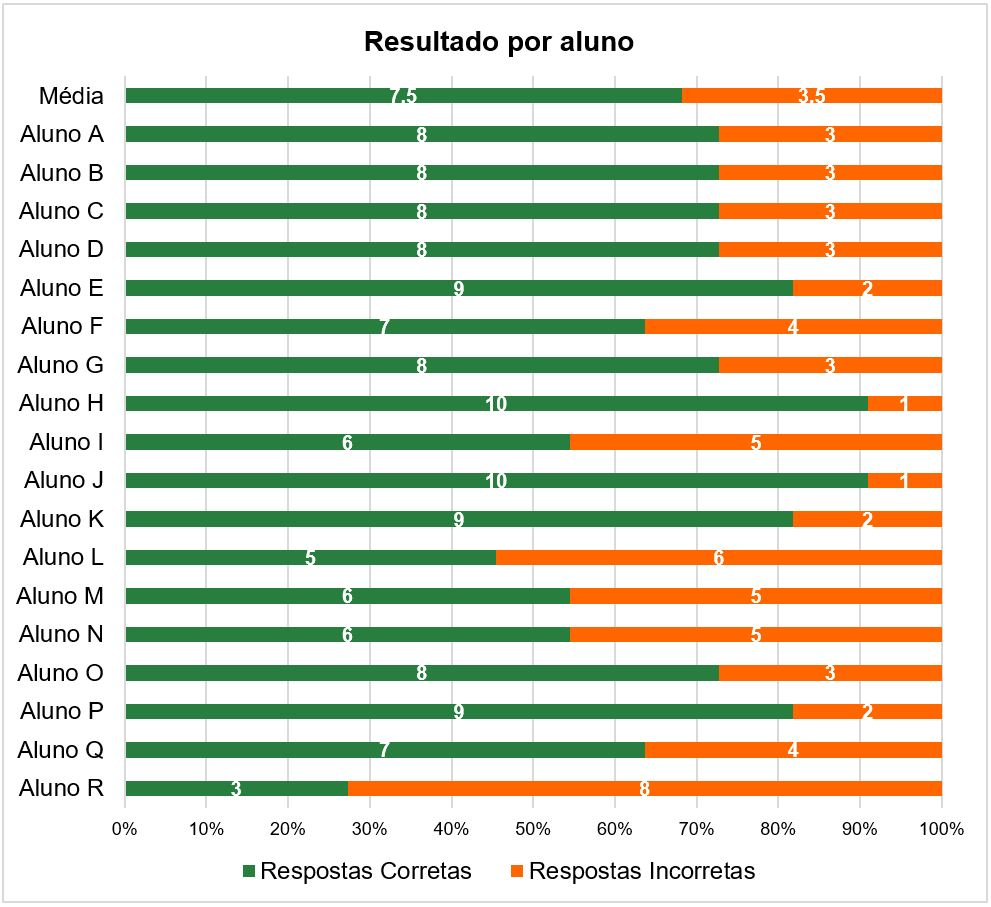
\includegraphics[width=0.9\textwidth]{g8-avaliacao-aprendizagem-resultado-aluno}
\legend{\footnotesize Fonte: Dados da pesquisa.}
\label{graf: g8-avaliacao-aprendizagem-resultado-aluno}
\end{minipage}
\end{grafico}

Percebe-se, portanto, através dos gráficos \ref{graf: g7-avaliação-aprendizagem-resultado-questão} e \ref{graf: g8-avaliacao-aprendizagem-resultado-aluno}, um nível bom de respostas corretas no Questionário de Avaliação de Aprendizagem (apêndice \ref{apend-a}), este resultado em conjunto com dados apresentados na avaliação dos jogos apontam que os alunos alcançaram, de modo geral, um bom nível de retenção sobre os principais temas apresentados durante o curso. Considerando os critérios avaliativos estabelecidos neste estudo, pode-se afirmar que a aprendizagem dos alunos foi efetiva já que a média de acerto dos estudantes e a média de acerto das questões foi ser superior ou igual a 60\%, critério este estabelecido considerando as normas do IFSUL.

\section{ANÁLISE DOS RESULTADOS DA AVALIAÇÃO DO CURSO}
O questionário de Avaliação do Curso foi idealizado a fim de aferir a efetividade do curso “Educação Financeira através de Jogos”, em conjunto com outros instrumentos, conforme os objetivos do presente trabalho. Ele possui oito questões dissertativas abertas e uma fechada de múltipla escolha. Os dados alcançados com as respostas dos alunos no questionário foram agrupados por questões e estão apresentadas em quadros no presente capítulo.

O quadro \ref{quad: quadro-23-motivou} apresenta as respostas dos alunos referente à primeira questão, “O que te motivou a participar deste curso?”. Por meio do retorno dos alunos nessa questão, é possível observar que o interesse dos alunos em participar do curso era compreender principalmente sobre investimentos e aprender administrar melhor o dinheiro, este interesse em aplicação financeira pode ser utilizado nas aulas de educação financeira para engajar os alunos para facilitar o processo de ensino-aprendizagem, inclusive da matemática financeira.

\graphicspath{{quadros/}} 
\begin{quadro}[!ht]
\centering
\begin{minipage}{0.8\textwidth}
\caption{Avaliação do Curso (Motivação dos Alunos)}
\centering
\includegraphics[width=0.80\textwidth]{quadro-23-motivou}
\legend{\footnotesize Fonte: Dados da pesquisa}
\label{quad: quadro-23-motivou}
\end{minipage}
\end{quadro}

O quadro \ref{quad: quadro-24-conhecimento} expõe as respostas dos estudantes referente à segunda questão do questionário, “Você conhecia os temas abordados nas aulas antes do curso? Se sim, quais temas?”. O \textit{feedback} dos alunos nessa questão demonstra que a maior parte dos alunos detinha conhecimento raso ou nenhum sobre os temas abordados antes do curso. Este fato em conjunto com interesse dos alunos por investimentos e em aprender administrar melhor suas finanças, pode indicar que os sujeitos da pesquisa se inscreveram no curso com o intuito de alcançar um conhecimento que não possuíam.

Normalmente, por não haver o ensino de educação financeira nas escolas, as crianças e adolescentes observam os hábitos financeiros dos pais, responsáveis ou pessoas próximas e os repetem em suas vidas \cite{herculano2005}, sejam eles corretos ou não. Por isso, o interesse dos alunos em participar de um curso de educação financeira, para administrar melhor suas finanças e investir, pode indicar que seus responsáveis também não possuem este conhecimento.

\graphicspath{{quadros/}} 
\begin{quadro}[!ht]
\centering
\begin{minipage}{0.8\textwidth}
\caption{Avaliação do Curso (Conhecimento Prévio)}
\centering
\includegraphics[width=0.85\textwidth]{quadro-24-conhecimento}
\legend{\footnotesize Fonte: Dados da pesquisa}
\label{quad: quadro-24-conhecimento}
\end{minipage}
\end{quadro}

O quadro \ref{quad: quadro-25-importância} apresenta as respostas dos alunos referente à terceira questão, “Você considera os temas abordados nas aulas importantes para seu futuro?”. Os alunos reconhecem a importância da educação financeira para seu futuro, fato que pode ser observado nas respostas dos estudantes na terceira pergunta e no interesse em participar do curso. Reconhecer esta importância é essencial, pois pode engajar os estudantes durante o ensino da educação financeira, o que colabora para a aprendizagem, formação de bons hábitos e comportamentos financeiros, os quais os alunos, possivelmente, levarão para o resto de suas vidas.

\graphicspath{{quadros/}} 
\begin{quadro}[!ht]
\centering
\begin{minipage}{0.8\textwidth}
\caption{Avaliação do Curso (Importância da Educação Financeira)}
\centering
\includegraphics[width=0.80\textwidth]{quadro-25-importância}
\legend{\footnotesize Fonte: Dados da pesquisa}
\label{quad: quadro-25-importância}
\end{minipage}
\end{quadro}

A pergunta do quadro \ref{quad: quadro-26-tecnologia-educacional} tem o objetivo de aferir a influência das tecnologias educacionais na aprendizagem. Todos os sujeitos da pesquisa responderam que de algum modo os jogos, ambientes virtuais e simuladores financeiros auxiliaram na aprendizagem. Os alunos relataram que as tecnologias educacionais auxiliaram na prática e na compreensão do conhecimento sobre investimentos, hábitos e comportamentos de consumo, administrar as finanças, importância do serviço de seguros, planejamento financeiro, importância de uma reserva de emergência financeira, gatilhos mentais e estratégias de venda.

As explanações dos estudantes, no quadro \ref{quad: quadro-26-tecnologia-educacional}, bem como as avaliações dos jogos com o método MEEGA+ confirmam a hipótese que as tecnologias educacionais utilizadas reproduziram ambientes financeiros seguros e lúdicos que facilitaram a compreensão dos alunos, tornando o conteúdo mais próximo dos estudantes, permitindo a prática, o aprendizado através da elaboração de soluções e na reflexão dos resultados alcançados nos jogos.

\graphicspath{{quadros/}} 
\begin{quadro}[!ht]
\centering
\begin{minipage}{0.80\textwidth}
\caption{Avaliação do Curso (Uso das Tecnologias Educacionais)}
\centering
\includegraphics[width=0.80\textwidth]{quadro-26-tecnologia-educacional}
\legend{\footnotesize Fonte: Dados da pesquisa}
\label{quad: quadro-26-tecnologia-educacional}
\end{minipage}
\end{quadro}

O sistema financeiro atual é algo complexo e dinâmico, por isso buscar novos conhecimentos é extremamente importante para acompanhar as mudanças. Nesse sentido, no quadro \ref{quad: quadro-27-novos-estudos} é possível observar que os alunos entenderam esta complexidade e se sentiram encorajados a buscar novos conhecimentos para aumentar suas experiências no mundo financeiro.

\graphicspath{{quadros/}} 
\begin{quadro}[!ht]
\centering
\begin{minipage}{0.80\textwidth}
\caption{Avaliação do Curso (Interesse em Novos Conhecimentos)}
\centering
\includegraphics[width=0.80\textwidth]{quadro-27-novos-estudos}
\legend{\footnotesize Fonte: Dados da pesquisa}
\label{quad: quadro-27-novos-estudos}
\end{minipage}
\end{quadro}

Ademais, analisando as respostas dos discentes no quadro \ref{quad: quadro-28-disseminação}, sobre a disseminação do conhecimento, observa-se que uma parte considerável dos discentes levaram o conhecimento adquirido sobre educação financeira no curso aos colegas, amigos e familiares. Considerando a baixa educação financeira da população brasileira e o interesse dos alunos em participar do curso, muito provavelmente, os assuntos abordados não fazem parte do convívio social da maior parcela dos sujeitos da pesquisa, demonstrar a importância durante do curso é essencial para que os estudantes disseminem o conhecimento adquirido à pessoas próximas, a fim de contribuir com a divulgar a educação financeira.

Desse modo, os resultados apresentados no quadro \ref{quad: quadro-28-disseminação} confirma que o curso contribuiu para a disseminação da educação financeira, atingindo não somente os alunos participantes do curso, mas também amigos, colegas, familiares e responsáveis, colaborando para o desenvolvimento da educação e do letramento financeiro.

\graphicspath{{quadros/}} 
\begin{quadro}[!ht]
\centering
\begin{minipage}{0.80\textwidth}
\caption{Avaliação do Curso (Disseminação do Conhecimento)}
\centering
\includegraphics[width=0.80\textwidth]{quadro-28-disseminação}
\legend{\footnotesize Fonte: Dados da pesquisa}
\label{quad: quadro-28-disseminação}
\end{minipage}
\end{quadro}

\newpage
Os principais motivos dos estudantes em participar do curso de “Educação Financeira através de Jogos” era aprender sobre investimentos e organização financeira. Outrossim, de acordo com as respostas expostas no quadro \ref{quad: quadro-29-temas-preferidos}, os alunos relataram que os temas preferidos, ou seja, que mais chamaram atenção no curso, foram principalmente investimentos e finanças comportamentais, esta última extremamente importante para organização financeira.

Portanto, os temas que motivaram os alunos a participar do curso foram os mesmos que mais chamaram atenção, este fato em conjunto com os relatos dos alunos no quadro \ref{quad: quadro-30-expectativas} demonstra que as expectativas dos alunos em relação ao curso foram atendidas, fator que provavelmente contribuiu para o engajamento dos alunos favorecendo assim o processo de ensino-aprendizagem no decorrer do curso.

\graphicspath{{quadros/}} 
\begin{quadro}[!ht]
\centering
\begin{minipage}{0.80\textwidth}
\caption{ Avaliação do Curso (Temas Preferidos do Curso)}
\centering
\includegraphics[width=0.80\textwidth]{quadro-29-temas-preferidos}
\legend{\footnotesize Fonte: Dados da pesquisa}
\label{quad: quadro-29-temas-preferidos}
\end{minipage}
\end{quadro}

\graphicspath{{quadros/}} 
\begin{quadro}[!ht]
\centering
\begin{minipage}{0.80\textwidth}
\caption{Avaliação do Curso (Atendimento às Expectativas)}
\centering
\includegraphics[width=0.80\textwidth]{quadro-30-expectativas}
\legend{\footnotesize Fonte: Dados da pesquisa}
\label{quad: quadro-30-expectativas}
\end{minipage}
\end{quadro}

\newpage
O quadro \ref{quad: quadro-31-observação} apresenta os dados levantados com a última pergunta do questionário cujo intuito do pesquisador era verificar comentários adicionais sobre o curso “Educação Financeira através de Jogos”. Por intermédio das respostas dos alunos, no retorno da questão, nota-se elogios em relação ao curso e a metodologia utilizada, sugestões de ampliação e adoção mais prática dos conhecimentos.

O pesquisador acredita na hipótese que as sugestões de uma adoção prática nas aulas seja referente aos investimentos, possivelmente os alunos gostariam de realizar aplicações financeiras reais em instituições financeira, principalmente em renda variável, entretanto é importante salientar que a maior parte dos alunos são menores de 18 anos e não respondem civilmente por suas decisões, por isso necessitam de autorização dos pais para realizarem investimentos, assim como que este curso foi elaborado para apresentar uma versão inicial sobre educação financeira, voltado principalmente para aquisição do conhecimento básico sobre finanças comportamentais, organização financeira e proteção dos alunos nas relações comerciais, esses conteúdos são elemento básico sobre finanças pessoais, por esse motivo é importante aprendê-los primeiro antes de adentrar nas investimentos, entretanto, nada impede que o conteúdo seja expandido para explorar e aprofundar mais os diversos tipos de aplicações em renda fixa e variável.

\graphicspath{{quadros/}} 
\begin{quadro}[!ht]
\centering
\begin{minipage}{0.80\textwidth}
\caption{Avaliação do Curso (Observação Sobre o Curso)}
\centering
\includegraphics[width=0.80\textwidth]{quadro-31-observação}
\legend{\footnotesize Fonte: Dados da pesquisa}
\label{quad: quadro-31-observação}
\end{minipage}
\end{quadro}

É importante considerar a motivação, os temas que mais chamaram a atenção, as expectativas, as sugestões de melhorias, elogios e críticas dos alunos em relação ao processo de ensino-aprendizagem, pois eles são os principais atores na educação. Deste modo, analisando o retorno dos alunos no questionário de avaliação pode-se afirmar que o curso proposto na presente pesquisa e sua metodologia assistida por tecnologias educacionais, principalmente a utilização de jogos sérios, foram bem avaliados pelos sujeitos da pesquisa e facilitaram a aprendizagem. Ademais, considerando os critérios para avaliar a efetividade do curso, estabelecidos no capítulo da metodologia, o curso “Educação Financeira através de Jogos” demonstrou-se ser efetivo para promover a educação financeira e o desenvolvimento do letramento financeiro dos estudantes da RFEPCT, pois a maior parcela dos alunos não tinham familiaridade com os temas apresentados, mesmo assim, apresentaram um bom nível de aprendizagem e retenção do conhecimento após o curso, demonstram interesse em buscar novos conhecimentos, disseminaram o conteúdo aprendido para amigos e familiares, para mais, o curso atendeu as expectativas dos alunos e utilizou de jogos que favoreceram a aprendizagem dos discentes, podendo ser expandido e ampliado para outras unidades da RFEPCT e redes de ensino para contribuir na diminuição dessa importante lacuna educacional.

\newpage
\section{ANÁLISE DOS RESULTADOS DA APLICAÇÃO DO CONHECIMENTO}
Conforme descrito em capítulo anteriores o questionário de aplicação do conhecimento é utilizado para indicar o possível estágio de desenvolvimento cognitivo do letramento financeiro de cada sujeito da pesquisa, verificar se os alunos e/ou seus familiares estão utilizando os conceitos financeiros adquiridos no curso, bem como averiguar de qual forma se esse conhecimento está auxiliando a superar os problemas financeiros causados pela pandemia do COVID-19.

Apenas o aluno R não respondeu o formulário digital do questionário de Aplicação do Conhecimento, o pesquisador do presente estudo empenhou-se em utilizar os meios de comunicação disponíveis para contatar o referido estudante, a fim de que este participasse da pesquisa, respondendo o questionário, entretanto o pesquisador não obteve êxito, por esse motivo a análise das respostas do questionário refere-se ao retorno de 17 alunos.

A primeira pergunta do questionário é referente à obtenção de recursos financeiros pelo aluno para utilizar em seu consumo, nesse sentido foi perguntado aos estudantes: “quais as fontes de dinheiro você utiliza para comprar produtos ou serviços?” Ao analisar as respostas dos alunos para esta pergunta (apêndice \ref{apend-d}) é possível verificar que 11 alunos possuem renda própria, adquirida através de estágio, trabalho formal e informal, bem como, que 6 alunos são dependentes dos pais e/ou bolsas estudantis para efetuar compra de produtos e serviços. A análise desses dados é importante para averiguar o perfil econômico dos estudantes, para ser analisado em conjunto dos hábitos e comportamentos financeiro dos estudantes.

A segunda pergunta do questionário é relacionada às mudanças que a participação no curso proporcionou na vida dos estudantes e de sua família. O quadro \ref{quad: quadro-32-mudança} apresenta o questionamento feito aos alunos e as respectivas respostas.

\graphicspath{{quadros/}}
\begin{quadro}[!ht]
\centering
\begin{minipage}{0.80\textwidth}
\caption{Aplicação do Conhecimento (Questão 2)}
\centering
\includegraphics[width=0.80\textwidth]{quadro-32-mudança}
\legend{\footnotesize Fonte: Dados da pesquisa}
\label{quad: quadro-32-mudança}
\end{minipage}
\end{quadro}

\newpage
Os relatos exibidos no quadro \ref{quad: quadro-32-mudança} indicam que após o curso os estudantes passaram a refletir mais sobre finanças e mudaram alguns hábitos financeiros, por meio do planejamento financeiro e do consumo consciente, fato que pode ser observado na resposta dos alunos A, B, D, E, F, H, J, K, L, M, P e Q. Há ainda estudantes que compreenderam a importância do controle e planejamento financeiro, mesmo não tendo ocorrido grandes mudanças em seu hábitos financeiro e de sua família, como os alunos C e O. Outro ponto importante, observado no quadro \ref{quad: quadro-32-mudança}, é a aproximação dos alunos com os investimentos, provavelmente este tema era algo muito distante dos discentes e com a participação no curso eles aprenderam sobre alguns tipos de aplicações financeiras e perceberam que investir pode ser algo atingível, esse resultado pode ser constatado através dos relatos dos alunos A, G, L, M, N e Q que descreveram sobre a aprendizagem de investimentos.

A terceira pergunta do questionário tem objetivo de verificar se o conteúdo trabalhado com os alunos no curso “Educação Financeira através de Jogos” tem ajudado aos alunos e seus familiares a enfrentar os problemas financeiros causados pela pandemia do COVID-19 e de qual modo. Nesse sentido, as respostas dos alunos referente a essa questão foram agrupadas e estão exibidas no quadro \ref{quad: quadro-33-covid}.

\graphicspath{{quadros/}}
\begin{quadro}[!ht]
\centering
\begin{minipage}{0.80\textwidth}
\caption{Aplicação do Conhecimento (Questão 3)}
\centering
\includegraphics[width=0.80\textwidth]{quadro-33-covid}
\legend{\footnotesize Fonte: Dados da pesquisa}
\label{quad: quadro-33-covid}
\end{minipage}
\end{quadro}

\newpage
Por intermédio da análise das respostas dos estudantes no quadro \ref{quad: quadro-33-covid} é possível afirmar que a participação no curso auxiliou a maior parte dos estudantes e de seus familiares a enfrentar as dificuldades financeiras causadas pela pandemia do COVID-19. Relatos acerca do consumo consciente, planejamento e controle financeiro (alunos B, C, D, E, F, G, H, K, L e O) demonstram a importância do conteúdo apresentado em sala no enfrentamento das adversidades financeiras. Por meio da organização financeira a família do aluno E, por exemplo, conseguiu inclusive ajudar parentes próximos, mesmo enfrentando dificuldade, outro exemplo interessante é a família do aluno F que depois do curso passou a diminuir o número de dívidas, fato que facilitou a enfrentar as dificuldades financeiras na pandemia. Esses relatos corroboram a importância de possibilitar o acesso ao conhecimento da educação financeira para os alunos do ensino médio integrado, no propósito de disponibilizar aos estudantes sabedoria necessária para enfrentar os desafios financeiros em sua vida e de sua família.

As questões número 4, 5, 6, 7 e 8 foram elaborados com o intuito de verificar em qual estágio do desenvolvimento cognitivo do letramento financeiro os alunos se encontravam após um ano de início do curso, de acordo com seus hábitos e comportamentos financeiros. As respostas completas de cada aluno são exibidas no apêndice \ref{apend-d}, o quadro \ref{quad: quadro-34-letramento-financeiro} apresenta um resumo correlacionando as respostas dos estudantes em relação aos hábitos financeiros com os estágios proposto por Peres et al. (\citeyear{peres2019}).

\graphicspath{{quadros/}}
\begin{quadro}[!ht]
\centering
\begin{minipage}{0.80\textwidth}
\caption{Aplicação do Conhecimento (Resultados)}
\centering
\includegraphics[width=0.80\textwidth]{quadro-34-letramento-financeiro}
\legend{\footnotesize Fonte: Dados da pesquisa}
\label{quad: quadro-34-letramento-financeiro}
\end{minipage}
\end{quadro}

\newpage
Ao observar o quadro \ref{quad: quadro-34-letramento-financeiro} é possível verificar que todos os 17 estudantes planejam, pesquisam e economizam dinheiro antes de efetuar a compra à vista de um produto ou serviço. Esse fato em conjunto com o baixo conhecimento prévio dos discentes demonstra que eles entenderam a importância de planejar o consumo e estão aplicando esse conhecimento em suas vidas. No quadro \ref{quad: quadro-34-letramento-financeiro} também é possível perceber que em relação ao registro de movimentação financeira 3 alunos não registram nenhuma movimentação e 14 anotam suas despesas e receitas, pois compreenderam a importância de anotar as movimentações financeiras e aplicam esse conhecimento em sua vida.

Segundo Peres et al. (\citeyear{peres2019}), no estágio Consumidor Sensorial o sujeito, normalmente, compra por impulso e não anota suas receitas e gastos. Ao analisar essa definição em conjunto com as repostas dos alunos no quadro \ref{quad: quadro-34-letramento-financeiro} é possível enquadrar 3 dos sujeitos de pesquisa nesse estágio de desenvolvimento cognitivo do letramento financeiro (alunos B, E e I, concentração na cor rosa no quadro \ref{quad: quadro-34-letramento-financeiro}), visto que não anotam suas movimentações financeiras o que normalmente dificulta o controle sobre o orçamento financeiro. Também é possível observar que os referidos alunos estão em um possível processo de ascensão ao próximo estágio (Consumidor Pré-poupador), uma vez que realizam a compra de bens, produtos e serviços de maneira planejada e consciente, diminuindo assim a ação do pensamento rápido \cite{kahneman2012}, a influência dos gatilhos mentais e as estratégias de vendas \cite{cialdini2012} nas tomadas de decisão de consumo, faltando lhes apenas o hábito de anotar as movimentações financeiras, a fim de elaborar um orçamento financeiro mais eficiente. Por outro lado, é possível inferir que os 14 estudantes restantes já emergiram para estágios posteriores do desenvolvimento cognitivo do letramento financeiro, pois registram suas movimentações financeiras e consomem de forma planejada.

No segundo estágio cognitivo do letramento financeiro definido por Peres et al. (\citeyear{peres2019}), Consumidor Pré-poupador, o sujeito pesquisa e planeja antes de adquirir produto, bens e serviços realizando o pagamento à vista ou a prazo dependendo do plano, também realiza um orçamento financeiro através do registro de receitas e despesas. Por intermédio dessa definição, do baixo conhecimento prévio dos alunos e do retorno dos alunos no questionário de aplicação do conhecimento, exibidos no quadro \ref{quad: quadro-34-letramento-financeiro}, é possível inferir que 14 alunos alcançaram o estágio Consumidor Pré-poupador do desenvolvimento cognitivo do letramento financeiro, pois possuem hábitos financeiros inerentes a esse estágio, percebe-se também, através do quadro \ref{quad: quadro-34-letramento-financeiro}, que 5 estudantes permanecem nessa fase do desenvolvimento e não evoluíram para estágios posteriores (aluno A, C, H, N e P, concentração em cor amarela no quadro \ref{quad: quadro-34-letramento-financeiro}).

De acordo com Peres et al. (\citeyear{peres2019}), no terceiro estágio do desenvolvimento cognitivo do letramento financeiro, intitulado Poupador Concreto, o sujeito, normalmente, realiza um bom orçamento financeiro, separa parte do dinheiro recebido no mês para investir e aplicar os recursos poupados apenas na caderneta de poupança por falta de conhecimento em outros investimentos. O quadro \ref{quad: quadro-34-letramento-financeiro} indica que 9 alunos ascenderam ao estágio de Poupador Concreto, pois apresentaram hábitos financeiros intrínseco à essa fase do desenvolvimento, o quadro \ref{quad: quadro-34-letramento-financeiro} também mostra que 4 alunos continuam nesse estágio desenvolvimento cognitivo do letramento financeiro (alunos F, G, L e Q, concentração na cor verde no quadro \ref{quad: quadro-34-letramento-financeiro}), não evoluindo ao próximo e último estágio.

No último estágio, Investidor Formal, o sujeito elabora metas e economiza parte do dinheiro adquirido para alcançar seus sonhos e objetivos, utiliza seu conhecimento em aplicação financeira para determinar o investimento mais adequado ao seu perfil e ao seu objetivo, diversificando suas aplicações em outros tipos de renda fixa ou em renda variável, não utilizando somente na caderneta de poupança (PERES et al., \citeyear{peres2019}). Nesse sentido ao analisar o quadro 34 pode-se concluir que 5 estudante atingiram o último estágio do desenvolvimento cognitivo do letramento financeiro (alunos D, J, K, M e O, concentração na cor azul no quadro \ref{quad: quadro-34-letramento-financeiro}), visto que indicaram em suas respostas hábitos financeiros pertinentes ao estágio Investidor Formal.

Assim sendo, observa-se por meio dos resultados apresentados no quadro \ref{quad: quadro-34-letramento-financeiro} que os alunos apresentaram uma evolução no letramento financeiro, mesmo que de forma tímida em alguns estudantes. Em resumo dos 18 alunos que realizaram o curso, sujeitos da presente pesquisa, 1 não respondeu o questionário de aplicação de conhecimento (aluno R), 3 estão no estágio Consumidor Sensorial (alunos B, E, I), 5 alcançaram o Consumidor Pré-Poupador (alunos A, C, H, N e P), 4 atingiram o Poupador Concreto (alunos F, G, L e Q) e 5 ascenderam ao estágio Investidor Formal (alunos D, J, K, M e O).

Independente do estágio de desenvolvimento cognitivo do letramento financeiro que o aluno se encontra é importante que este mantenha seus estudos sobre finanças, pois, conforme visto em capítulos anteriores, o mundo financeiro é algo complexo e dinâmico, portanto, somente o aprendizado contínuo poderá fornecer ferramentas necessárias para enfrentar os desafios financeiros que surgem constantemente na vida das pessoas na sociedade contemporânea.

\chapter{CONSIDERAÇÕES FINAIS}
Este projeto apresentou uma proposta de um curso para introdução da educação financeira que emprega uma metodologia assistida por tecnologias educacionais como simuladores, ambientes virtuais e, principalmente, jogos sérios, para auxiliar na consolidação da educação financeira nos cursos técnicos integrados da RFEPCT. O conteúdo apresentado no curso de “Educação Financeira através de Jogos” proporcionou aos alunos participantes o conhecimento introdutório sobre finanças, extremamente necessário para o letramento financeiro, abrangendo do primeiro ao último estágio de desenvolvimento cognitivo do letramento financeiro descritos no referencial teórico: Consumidor Sensorial, Consumidor Pré-Poupador, Poupador Concreto e Investidor Formal.

O presente trabalho apoiou-se em fundamentos teóricos educacionais e tecnológicos para possibilitar o seu uso efetivo, visando complementar a formação do estudante do ensino médio integrado em um tema ainda pouco explorado, o qual impacta diretamente ao longo da vida de todas as pessoas, principalmente na presente sociedade contemporânea e tecnológica, desta forma, o trabalho possui potencial para ser ampliado, pesquisado e aplicado em outras redes de ensino.

Foram disponibilizadas 19 vagas para o curso de “Educação Financeira através de Jogos” no IFSUL Câmpus Gravataí para os alunos do ensino médio integrado da instituição, embora o curso tenha sido oferecido por um projeto de ensino como disciplina não obrigatória, 41 alunos da instituição se inscreveram para participar da formação, a quantidade de interessados que solicitaram inscrição no curso surpreendeu positivamente os autores deste estudo e demonstra uma procura relevante pelo assunto. A demanda reprimida do curso levou à necessidade de realizar sorteio para preencher as vagas que, mesmo com uma divulgação considerada tímida, mobilizou 15\% dos alunos de ensino médio integrado do câmpus. Possivelmente, no mundo contemporâneo globalizado e conectado, os jovens estudantes estejam mais conscientes sobre a importância da educação financeira, mas ainda lhes faltam ambientes e oportunidades para o aprendizado de forma efetiva.

\section{CONTRIBUIÇÕES DO PROJETO}
A presente pesquisa contribuiu para a disseminação da educação financeira e para promover o conhecimento financeiro e incentivar o desenvolvimento do letramento financeiro dos sujeitos da pesquisa, de seus familiares e amigos, colaborou para estabelecer um caminho e uma abordagem educacional visando o ensino da educação financeira, estruturado a partir do desenvolvimento cognitivo do letramento financeiro, demonstrou que os jogos e os simuladores são tecnologias educacionais que podem facilitar o processo de ensino-aprendizagem, bem como comprovou que os jogos Orçamento Consciente e Renda Passiva podem ser utilizados em aulas introdutórias sobre educação financeira. Em algumas famílias dos alunos participantes, o conhecimento adquirido no curso ajudou a administrar de forma mais assertiva o orçamento familiar, no propósito de enfrentar as dificuldades financeiras causadas pela pandemia do COVID-19.

\section{PERSPECTIVAS FUTURAS}
Espera-se que os resultados do presente trabalho possam impactar no processo de ensino-aprendizagem da educação financeira no ensino médio da RFEPCT e de outras redes de ensino, bem como, que o curso possa ser usado amplamente por instituições de ensino brasileiras, evoluindo-o e integrando-o definitivamente aos currículos do ensino médio, contribuindo efetivamente com o desenvolvimento do letramento financeiro dos estudantes e com novos estudos acerca do tema de pesquisa. Almeja-se também com este trabalho, colaborar para a formação sólida e ampla dos estudantes profissionais, para que possam enfrentar os desafios impostos pela sociedade atual, que exige dos cidadãos mais conhecimento sobre economia, finanças e tecnologia.

% ==============================================
% ELEMENTOS PÓS-TEXTUAIS
% ==============================================
\postextual
% ||||||||||||||||||||||||||||||||||||||||||||||
% REFERÊNCIAS BIBLIOGRÁFICAS
% ||||||||||||||||||||||||||||||||||||||||||||||
%\bibliography{bibfile2}
% bibliografia john
\bibliography{ref-bibliografica}
% ----------------------------------------------
% Glossário
% ----------------------------------------------
% Consulte o manual da classe abntex2 para orientações sobre o glossário.
%
%\glossary
% ||||||||||||||||||||||||||||||||||||||||||||||
% APÊNDICES
% ||||||||||||||||||||||||||||||||||||||||||||||
% Imprime uma página indicando o início dos apêndices
%\partapendices
% ----------------------------------------------
% Apêndice
% ----------------------------------------------
\begin{apendicesenv}
    \chapter{Avaliação da Aprendizagem}\label{apend-a}
    \begin{enumerate}
    \item O que é a educação financeira?
    
    \item Qual as características de um bom orçamento financeiro?
    
    \item Considerando a Educação Financeira e a Matemática Financeira assinale a alternativa correta:
        \begin{enumerate}
            \item  (   ) A Educação Financeira promove reflexão sobre a vida financeira.
           \item   (   ) A Matemática Financeira trata sobre hábitos financeiros.
            \item  (   ) A Matemática Financeira aborda os tipos de investimentos.
            \item  (   ) A Educação Financeira e a Matemática Financeira são sinônimos.
        \end{enumerate}
    
    \item Selecione a alternativa correta. O orçamento pessoal ou familiar auxilia:
        \begin{enumerate} 
            \item (   ) No controle de receitas e despesas
            \item (   ) Administrar os recursos financeiros de forma consciente
            \item (   ) No controle das dívidas
            \item (   ) Todas as alternativas anteriores
        \end{enumerate}
        
    \item Abaixo há uma lista de itens relacionados às necessidades, desejos e desperdício. Assinale as alternativas referentes somente às necessidades, pode-se escolher mais de uma alternativa.
        \begin{enumerate}
            \item (   ) Sapato de marca - Cirurgia plástica
            \item (   ) Passagem de ônibus - Remédio
            \item (   ) Restaurantes - Viagens - Carro do ano
            \item (   ) Aluguel da casa - Roupas - Lazer
        \end{enumerate}
    
    \item Escolha a alternativa abaixo que representa a ordem das etapas de um Orçamento Financeiro.
        \begin{enumerate}
            \item (   ) Avaliar, Agrupar, Planejar e Registrar
            \item (   ) Registrar, Planejar, Avaliar, Agrupar
            \item (   ) Planejar, Registrar, Agrupar e Avaliar
            \item (   ) Registrar, Agrupar, Planejar e Avaliar
        \end{enumerate}
    
    \newpage    
    \item Qual o tipo de juros é utilizado para rentabilidade dos investimentos?
        \begin{enumerate}
            \item (   ) Juros Simples
            \item (   ) Juros de Mora
            \item (   ) Juros Compostos
            \item (   ) Juros de Capital Próprio
        \end{enumerate}
        
    \item Considerando que a inflação é a variação mensal dos preços, marque a alternativa que representa o índice oficial que o governo brasileiro utiliza para medir a inflação nacional.
        \begin{enumerate}
            \item (   ) CDI
            \item (   ) SELIC
            \item (   ) CDB
            \item (   ) IPCA
        \end{enumerate}
        
    \item Investimento é aplicação do dinheiro poupado para obtenção de juros ou dividendos. Eles possuem três característica Risco, Rentabilidade e Liquidez. Sabendo disso assinale a alternativa que corresponde a definição de Liquidez.
        \begin{enumerate}
            \item (   ) É a probabilidade de ocorrer perdas no investimento
            \item (   ) É a possibilidade do investimento ser transformado em dinheiro
            \item (   ) É a remuneração recebida pelo investimento
        \end{enumerate}
        
    \item Assinale a alternativa cujo investimento não é garantido pelo FGC.
        \begin{enumerate}
            \item (   ) Tesouro Direto
            \item (   ) LCI/LCA
            \item (   ) CDB
            \item (   ) Poupança
        \end{enumerate}
        
    \item Assinale a características de um Investimento em Renda Variável.
        \begin{enumerate}
            \item (   ) Esse tipo de investimento não possui riscos 
            \item (   ) A rentabilidade desse investimento é garantida
            \item (   ) Esse tipo de investimento possui riscos
            \item (   ) É coberto pelo Fundo Garantidor de Crédito
        \end{enumerate}
\end{enumerate}

    
    \chapter{Avaliação do Curso}\label{apend-b}
    \begin{enumerate}
    \item O que te motivou a participar deste curso?
    
    \item Você conhecia os temas abordados nas aulas antes do curso? Se sim, quais temas?
    
    \item Você considera os temas abordados nas aulas importantes para o seu futuro?
    
    \item Os simuladores, jogos (físicos e digitais) e os ambientes virtuais auxiliaram na compreensão dos assuntos abordados durante as aulas? Caso sim de qual forma?
    
    \item Você tem interesse em buscar de novos conhecimentos sobre os temas abordados nas aulas?
    
    \item Você conversou com sua família ou amigos ou parentes sobre o curso? Se sim com quem e quais temas?
    
    \item Quais os temas do curso que mais gostou?
    
    \item O curso está atendendo as suas expectativas.
        \begin{enumerate}
            \item Concordo Totalmente
            \item Concordo Parcialmente
            \item Indiferente
            \item Discordo Parcialmente
            \item Discordo Totalmente
        \end{enumerate}
    
    \item Há alguma sugestão de melhoria, elogio e/ou crítica que gostaria de fazer em relação ao curso?
\end{enumerate}
    
    \chapter{Aplicação do Conhecimento}\label{apend-c}
    Em relação à sua vida financeira atual responda às seguintes perguntas:
\begin{enumerate}
   \item Quais as fontes de dinheiro você utiliza para comprar produtos ou serviços? (Ex: trabalho, estágio, bolsa de estudo, auxílio escolar, mesada, dinheiro dado pelos responsáveis quando necessita, pensão etc).
   
   \item A sua participação no curso de Educação Financeira proporcionou quais mudanças em sua vida e de sua família?
   
   \item De que forma o conhecimento adquirido no curso está auxiliando você e sua família a enfrentar os problemas financeiros causado pela pandemia do COVID-19?
   
   \item Como normalmente você realiza a compra de produtos e serviços?
        \begin{enumerate}
            \item Compro por impulso quando tenho dinheiro para comprar à vista
            \item Compro por impulso e parcelo no cartão de crédito
            \item Planejo, pesquiso e economizo dinheiro antes de comprar à vista
            \item Planejo, pesquiso antes de comprar parcelado no cartão
            \item Outros:
        \end{enumerate}
        
    \item Como você controla suas receitas e gastos mensais?
        \begin{enumerate}
            \item Não anoto nenhum gasto ou receita mensal
            \item Registro todos os gastos e receitas que possuo
            \item Registro apenas gastos e receitas grandes
            \item Outros:
        \end{enumerate}
        
    \item Você separa parte do dinheiro recebido para investir?
        \begin{enumerate}
            \item Sim, antes de gastar
            \item Sim, se sobrar
            \item Não, sempre utilizo todo dinheiro que ganho
            \item Outros:
        \end{enumerate}
    
    \item Normalmente em qual tipo de investimento você aplica o dinheiro poupado? (É possível marcar mais de uma opção).
        \begin{enumerate}
            \item Não poupo dinheiro para aplicar
            \item Caderneta de poupança
            \item Outros investimentos de renda fixa
            \item Investimentos de renda variável
            \item Outros:
        \end{enumerate}
        
    \item Você planeja e economiza parte do dinheiro recebido para sonhos e objetivos futuros?
        \begin{enumerate}
            \item Não, vivo apenas o presente
            \item Não, pois nunca sobra dinheiro
            \item Sim, tenho metas, poupo e aplico dinheiro para objetivos futuros
            \item Outros:
        \end{enumerate}
\end{enumerate}
    
    \chapter{APLICAÇÃO DO CONHECIMENTO - RESPOSTAS}\label{apend-d}
    \includepdf[pages=-]{apendices/aplicacao-conhecimento-resposta.pdf}
    
%\includepdf[pages=-]{apendices/apendice.pdf}

\end{apendicesenv}

% ||||||||||||||||||||||||||||||||||||||||||||||
% ANEXOS
% ||||||||||||||||||||||||||||||||||||||||||||||
%\begin{anexosenv}
% Imprime uma página indicando o início dos anexos
%\partanexos
% ----------------------------------------------
% Anexo 1
% ----------------------------------------------
%\chapter{Datasheet}\label{anexo1}
%\includepdf[pages=-]{pdfs/Datasheet.pdf}
% ----------------------------------------------
% Anexo 2
% ----------------------------------------------
%\chapter{Anexo 2}
%\end{anexosenv}
% ==============================================
% INDICE REMISSIVO
% ==============================================
\phantompart
\printindex
% ----------------------------------------------
% ||||||||||||||||||||||||||||||||||||||||||||||
% DOCUMENTO PARA ENTREGA VERSÃO FINAL
%||||||||||||||||||||||||||||||||||||||||||||||
\begin{comment}

\clearpage\thispagestyle{empty}\addtocounter{page}{-1}
\section*{ENTREGA DA VERSÃO FINAL DE DISSERTAÇÃO}

\vspace*{2cm}
Eu, \textsc{\imprimirorientador}, autorizo o aluno(a) \textsc{\imprimirautor} a entregar a versão final da dissertação de mestrado, à secretaria do MPIE, que foi por mim analisada e está de acordo com os apontamentos feitos pelos membros da banca de apresentação do referido aluno.

\vspace*{1cm}
\begin{center}   
   \assinatura{{\imprimirorientador} \\ Orientador}
\end{center}

\vspace*{1cm}
\begin{flushright}
	\imprimirlocal, 11 de Julho de \imprimirdata.
\end{flushright}
\clearpage
\end{comment}

\end{document}